\documentclass[../thesis.tex]{subfiles}
\begin{document}

\chapter{parametric study}
\label{chp: para_stud}
Within the parametric study the three different reactor geometries are simulated under different flow conditions. These different conditions, as shown in \autoref{tab: cases}, lead to different front shapes. Two of these front shapes can be seen in \autoref{fig: shape_examp}.
\begin{figure}[htb]
	\centering
	\subfloat[\centering front shape for h0.6mm Pe2050 Sc12000]{{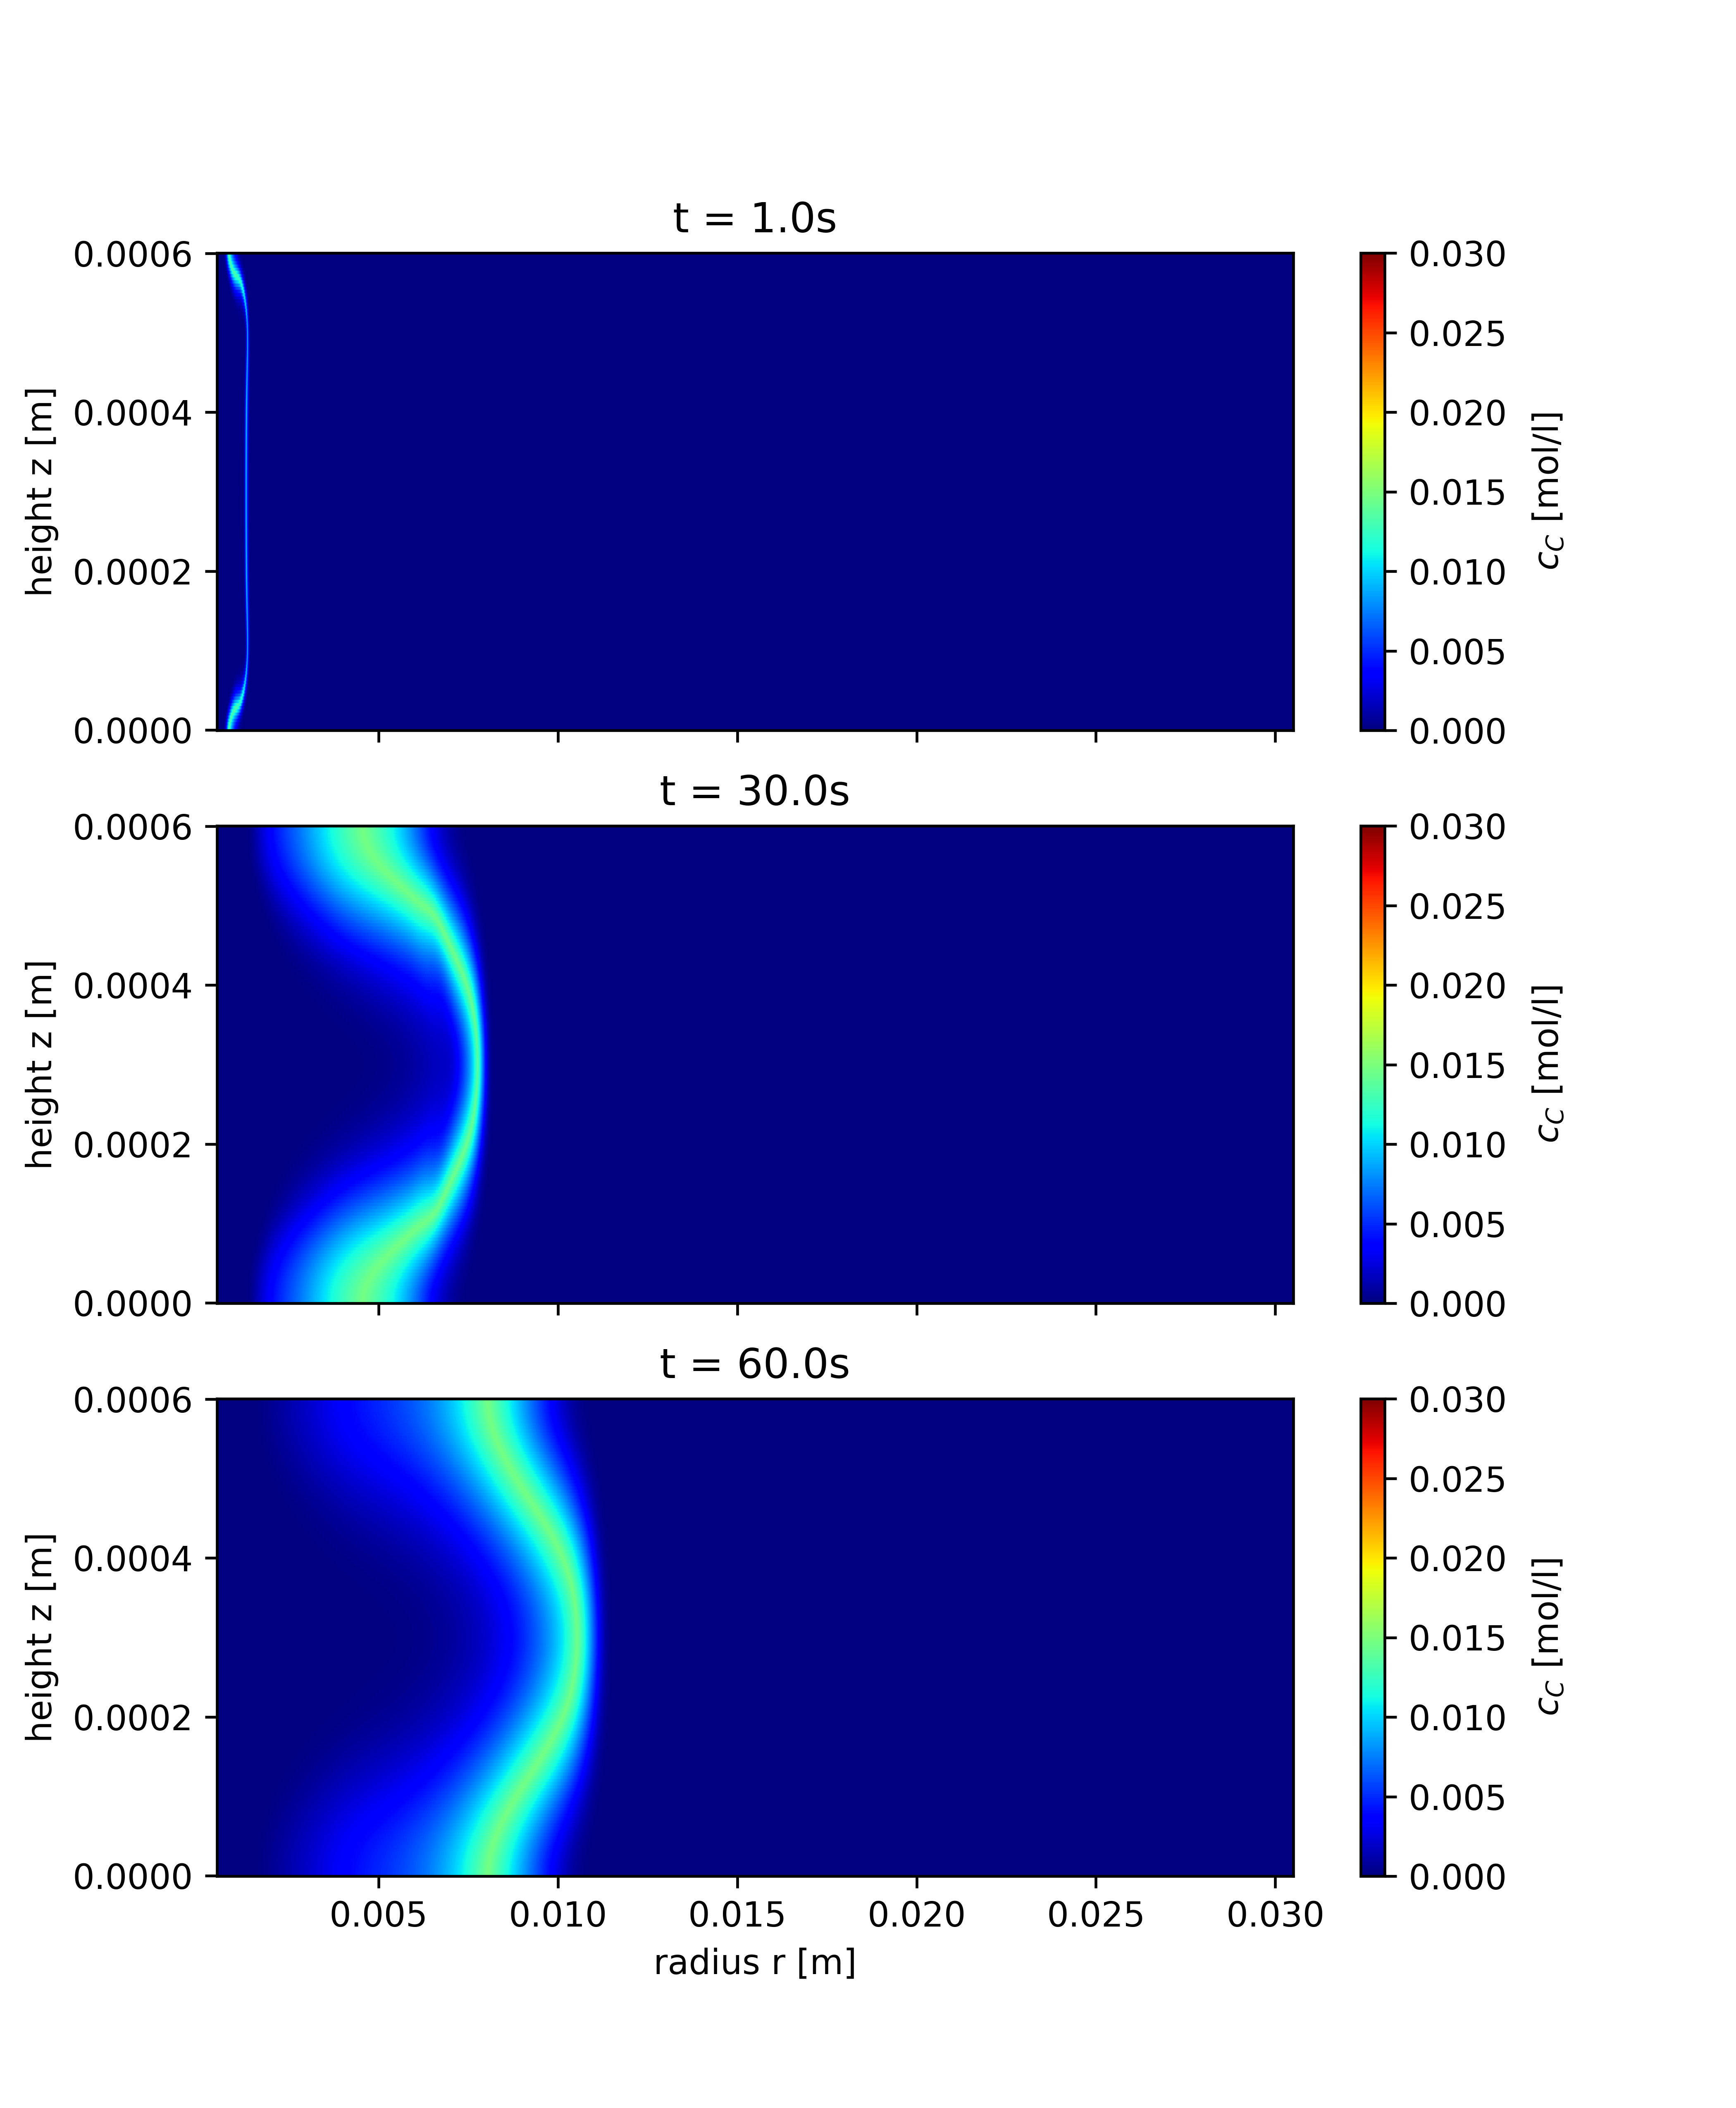
\includegraphics[angle=0, scale=0.41]{front_shape1} }}%
	\qquad
	\subfloat[\centering front shape for h0.2mm Pe2050 Sc2430]{{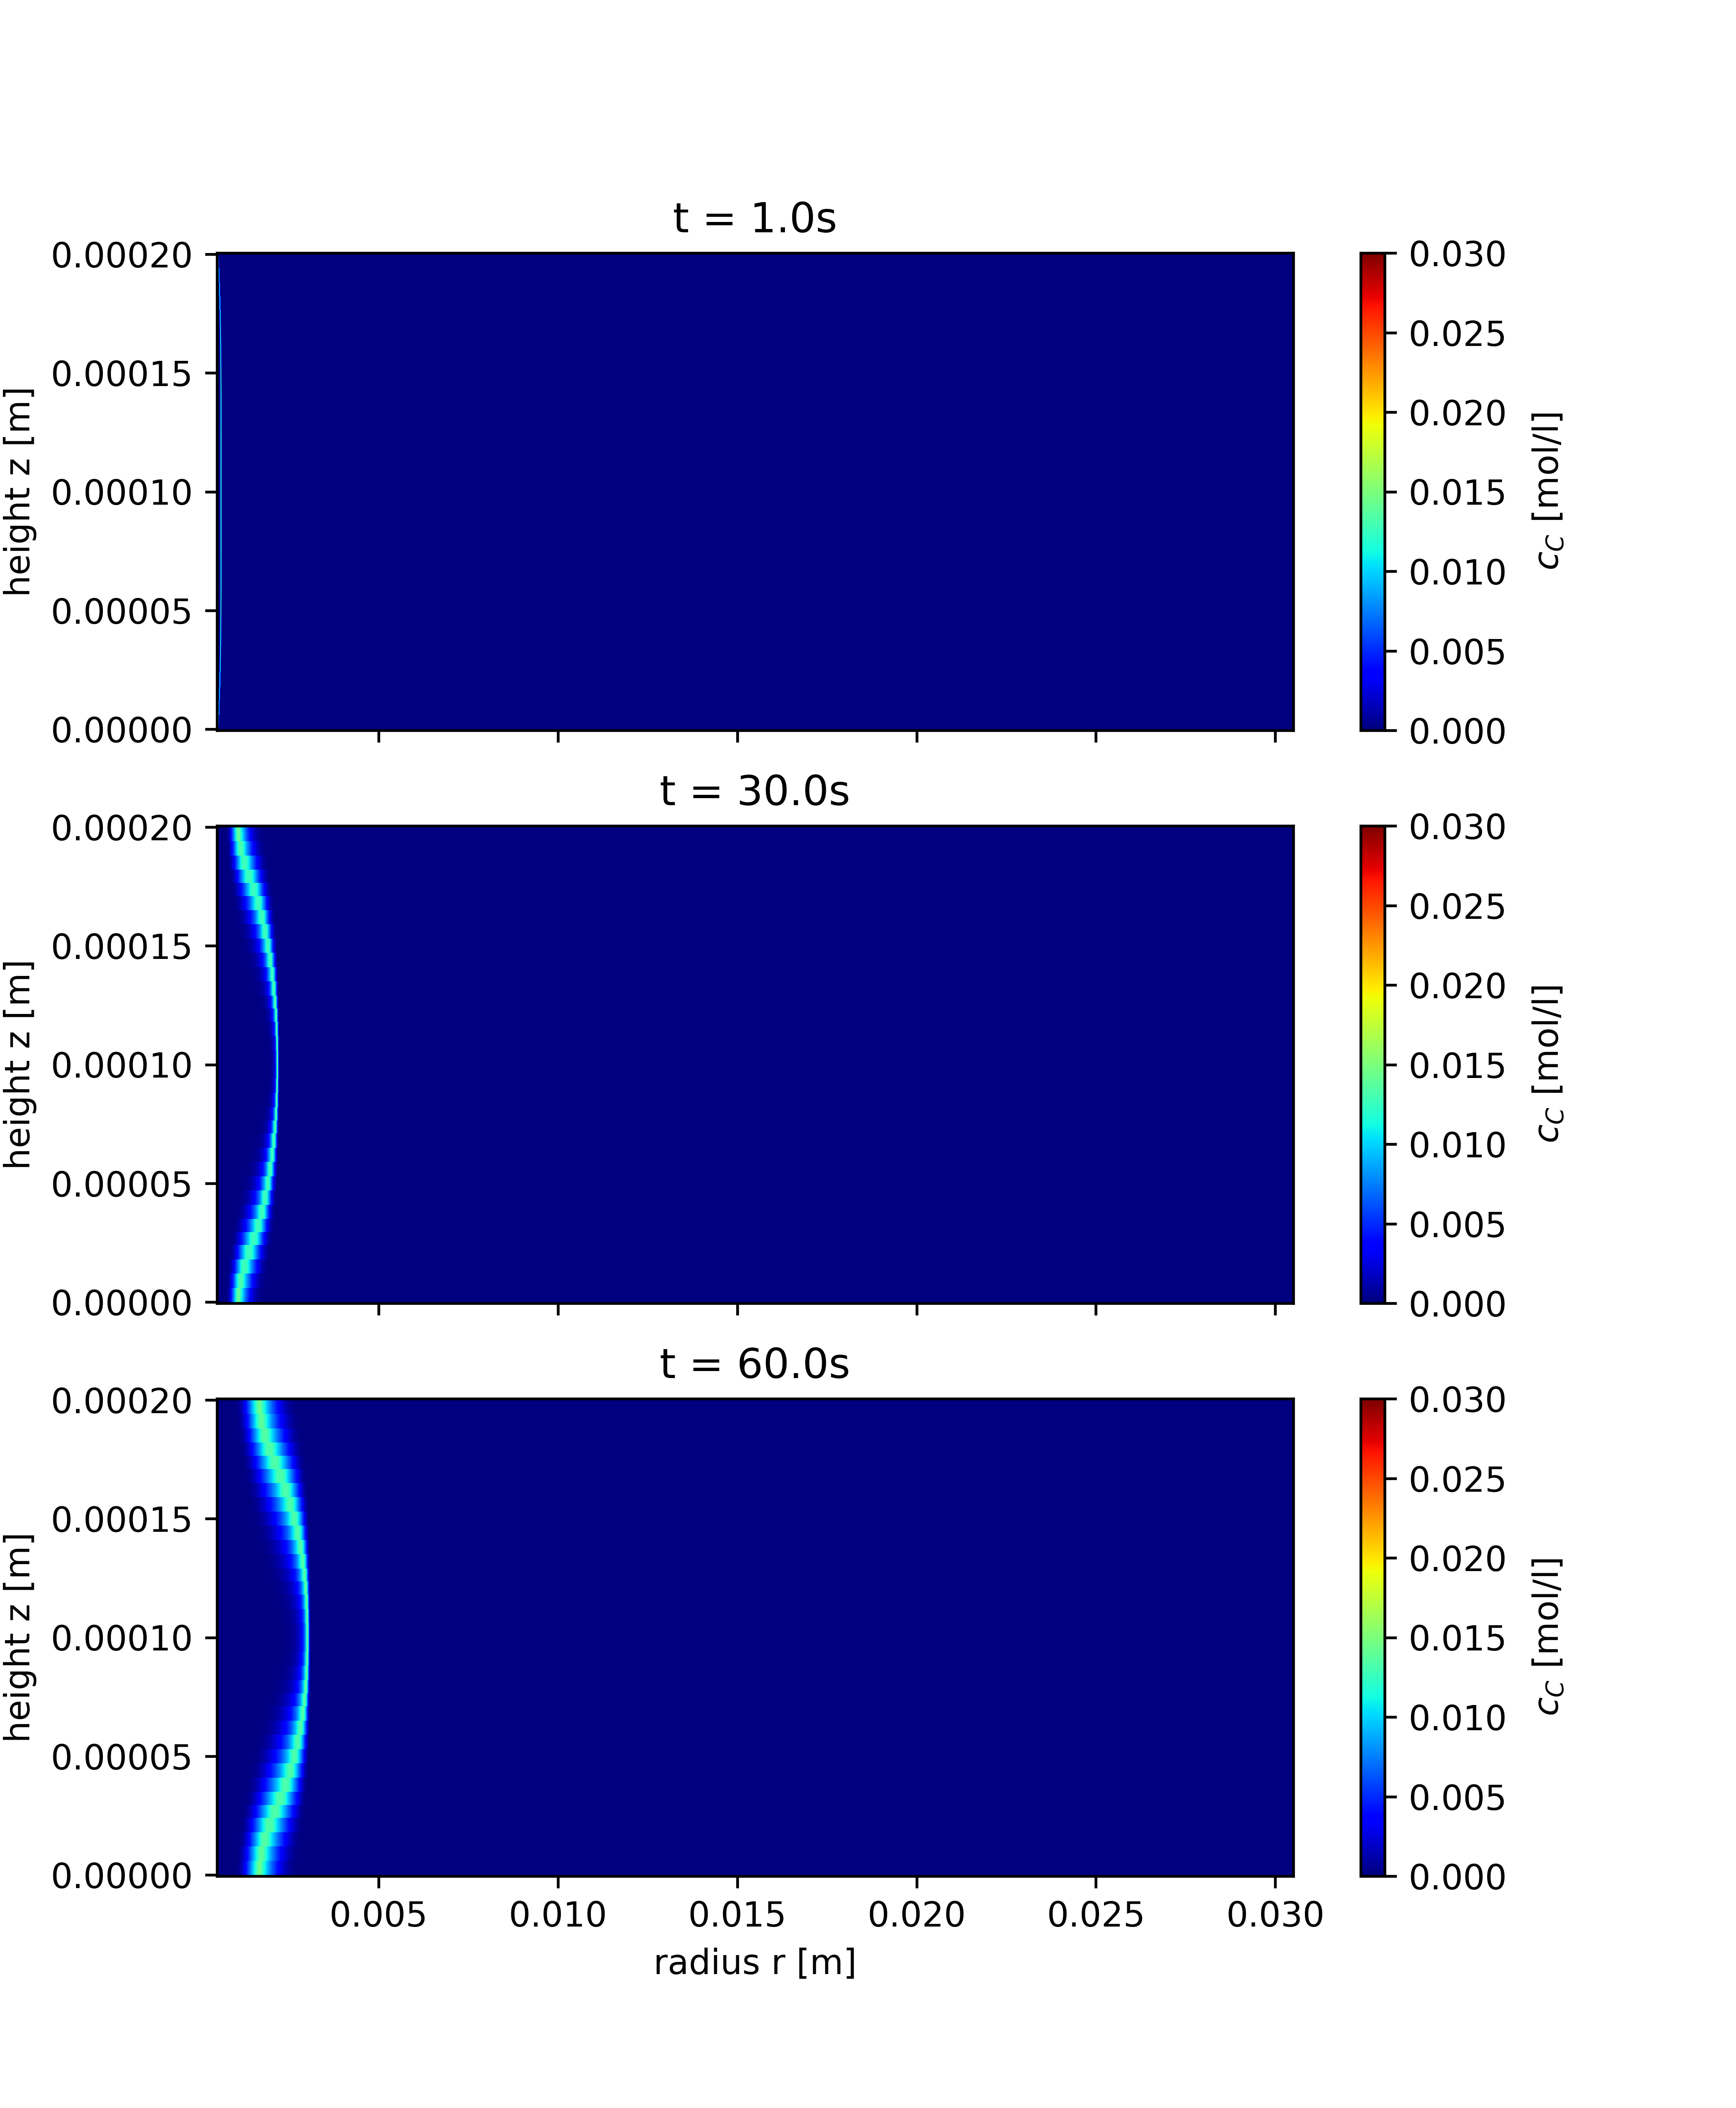
\includegraphics[angle=0, scale=0.41]{front_shape2} }}%
	\caption{example front shapes}%
	\label{fig: shape_examp}%
\end{figure}

\section{front positions}

The front positions behave in a similar way for all 3 reactor geometries. So in \autoref{fig: front_pos_h2_Sc12000} and \autoref{fig: front_pos_h2_Sc2430} the positions for both Schmidt-Number are shown for the geometry containing a gap height of 0.2mm.
% two figures on same page
\begin{figure}[htbp]
	\centering
	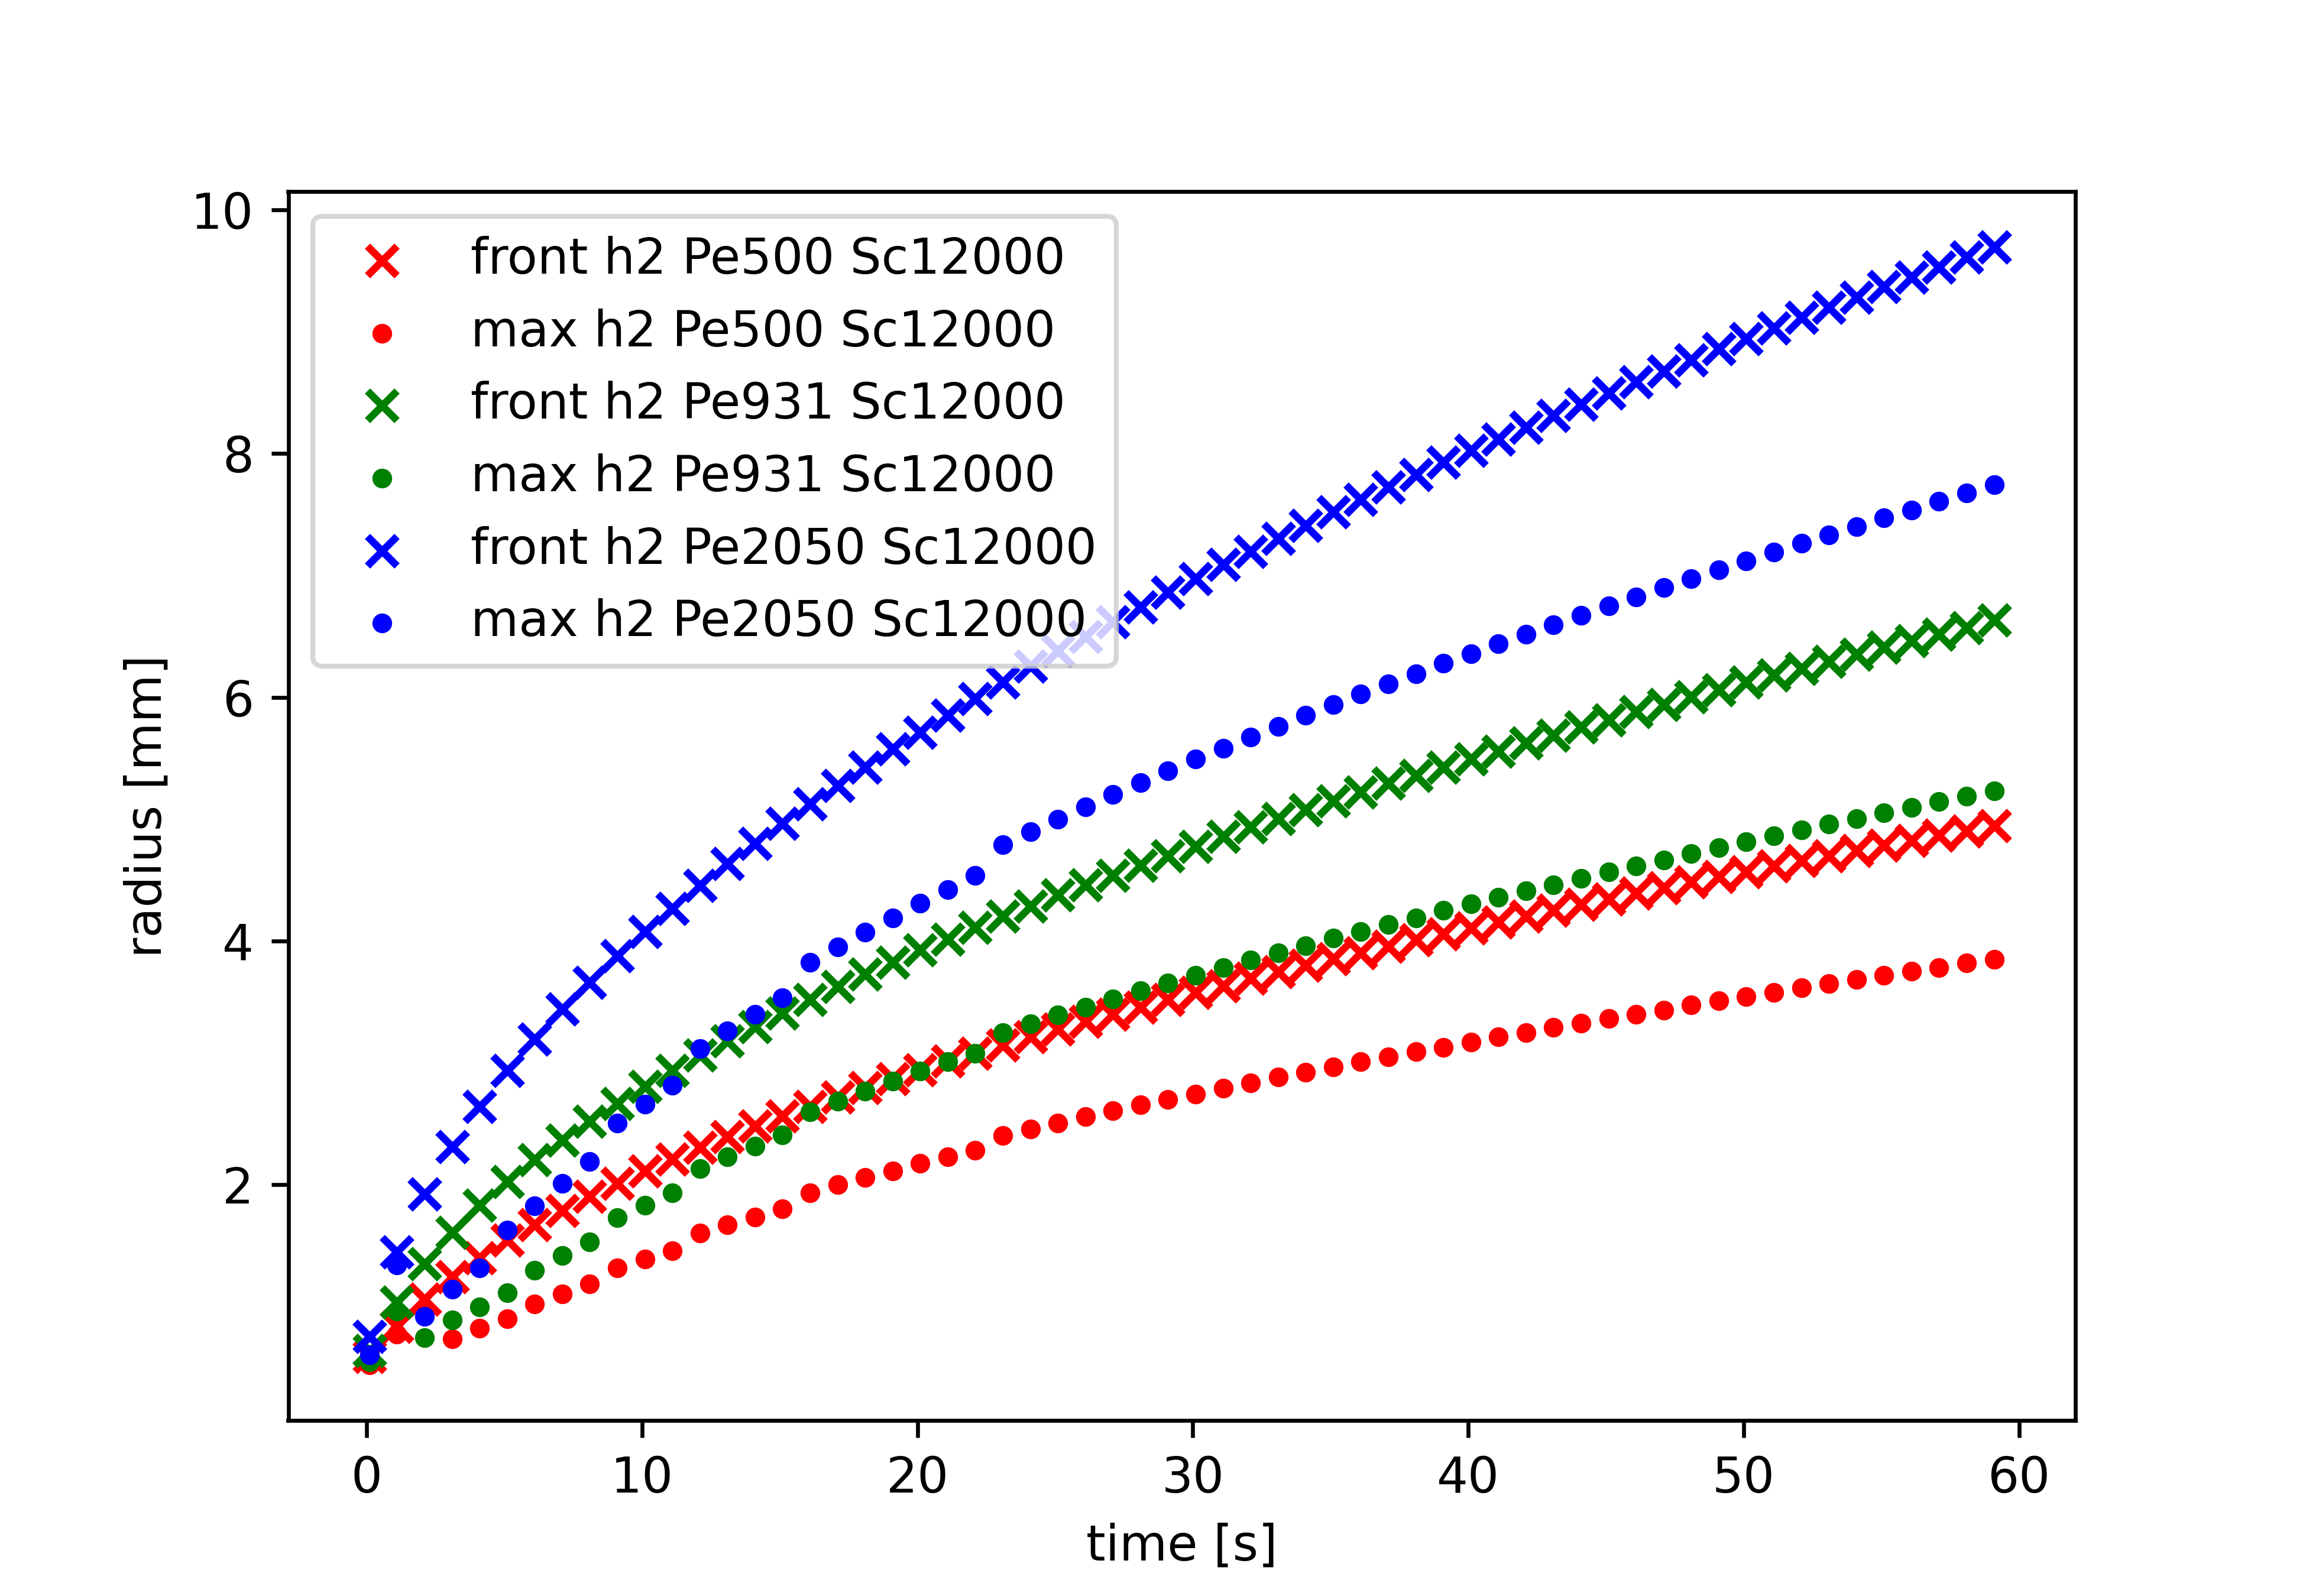
\includegraphics[width=.9\linewidth]{front_pos_h2_Sc12000}
	\caption{front positions for h 0.2mm Sc 12000\label{fig: front_pos_h2_Sc12000}}\bigskip
	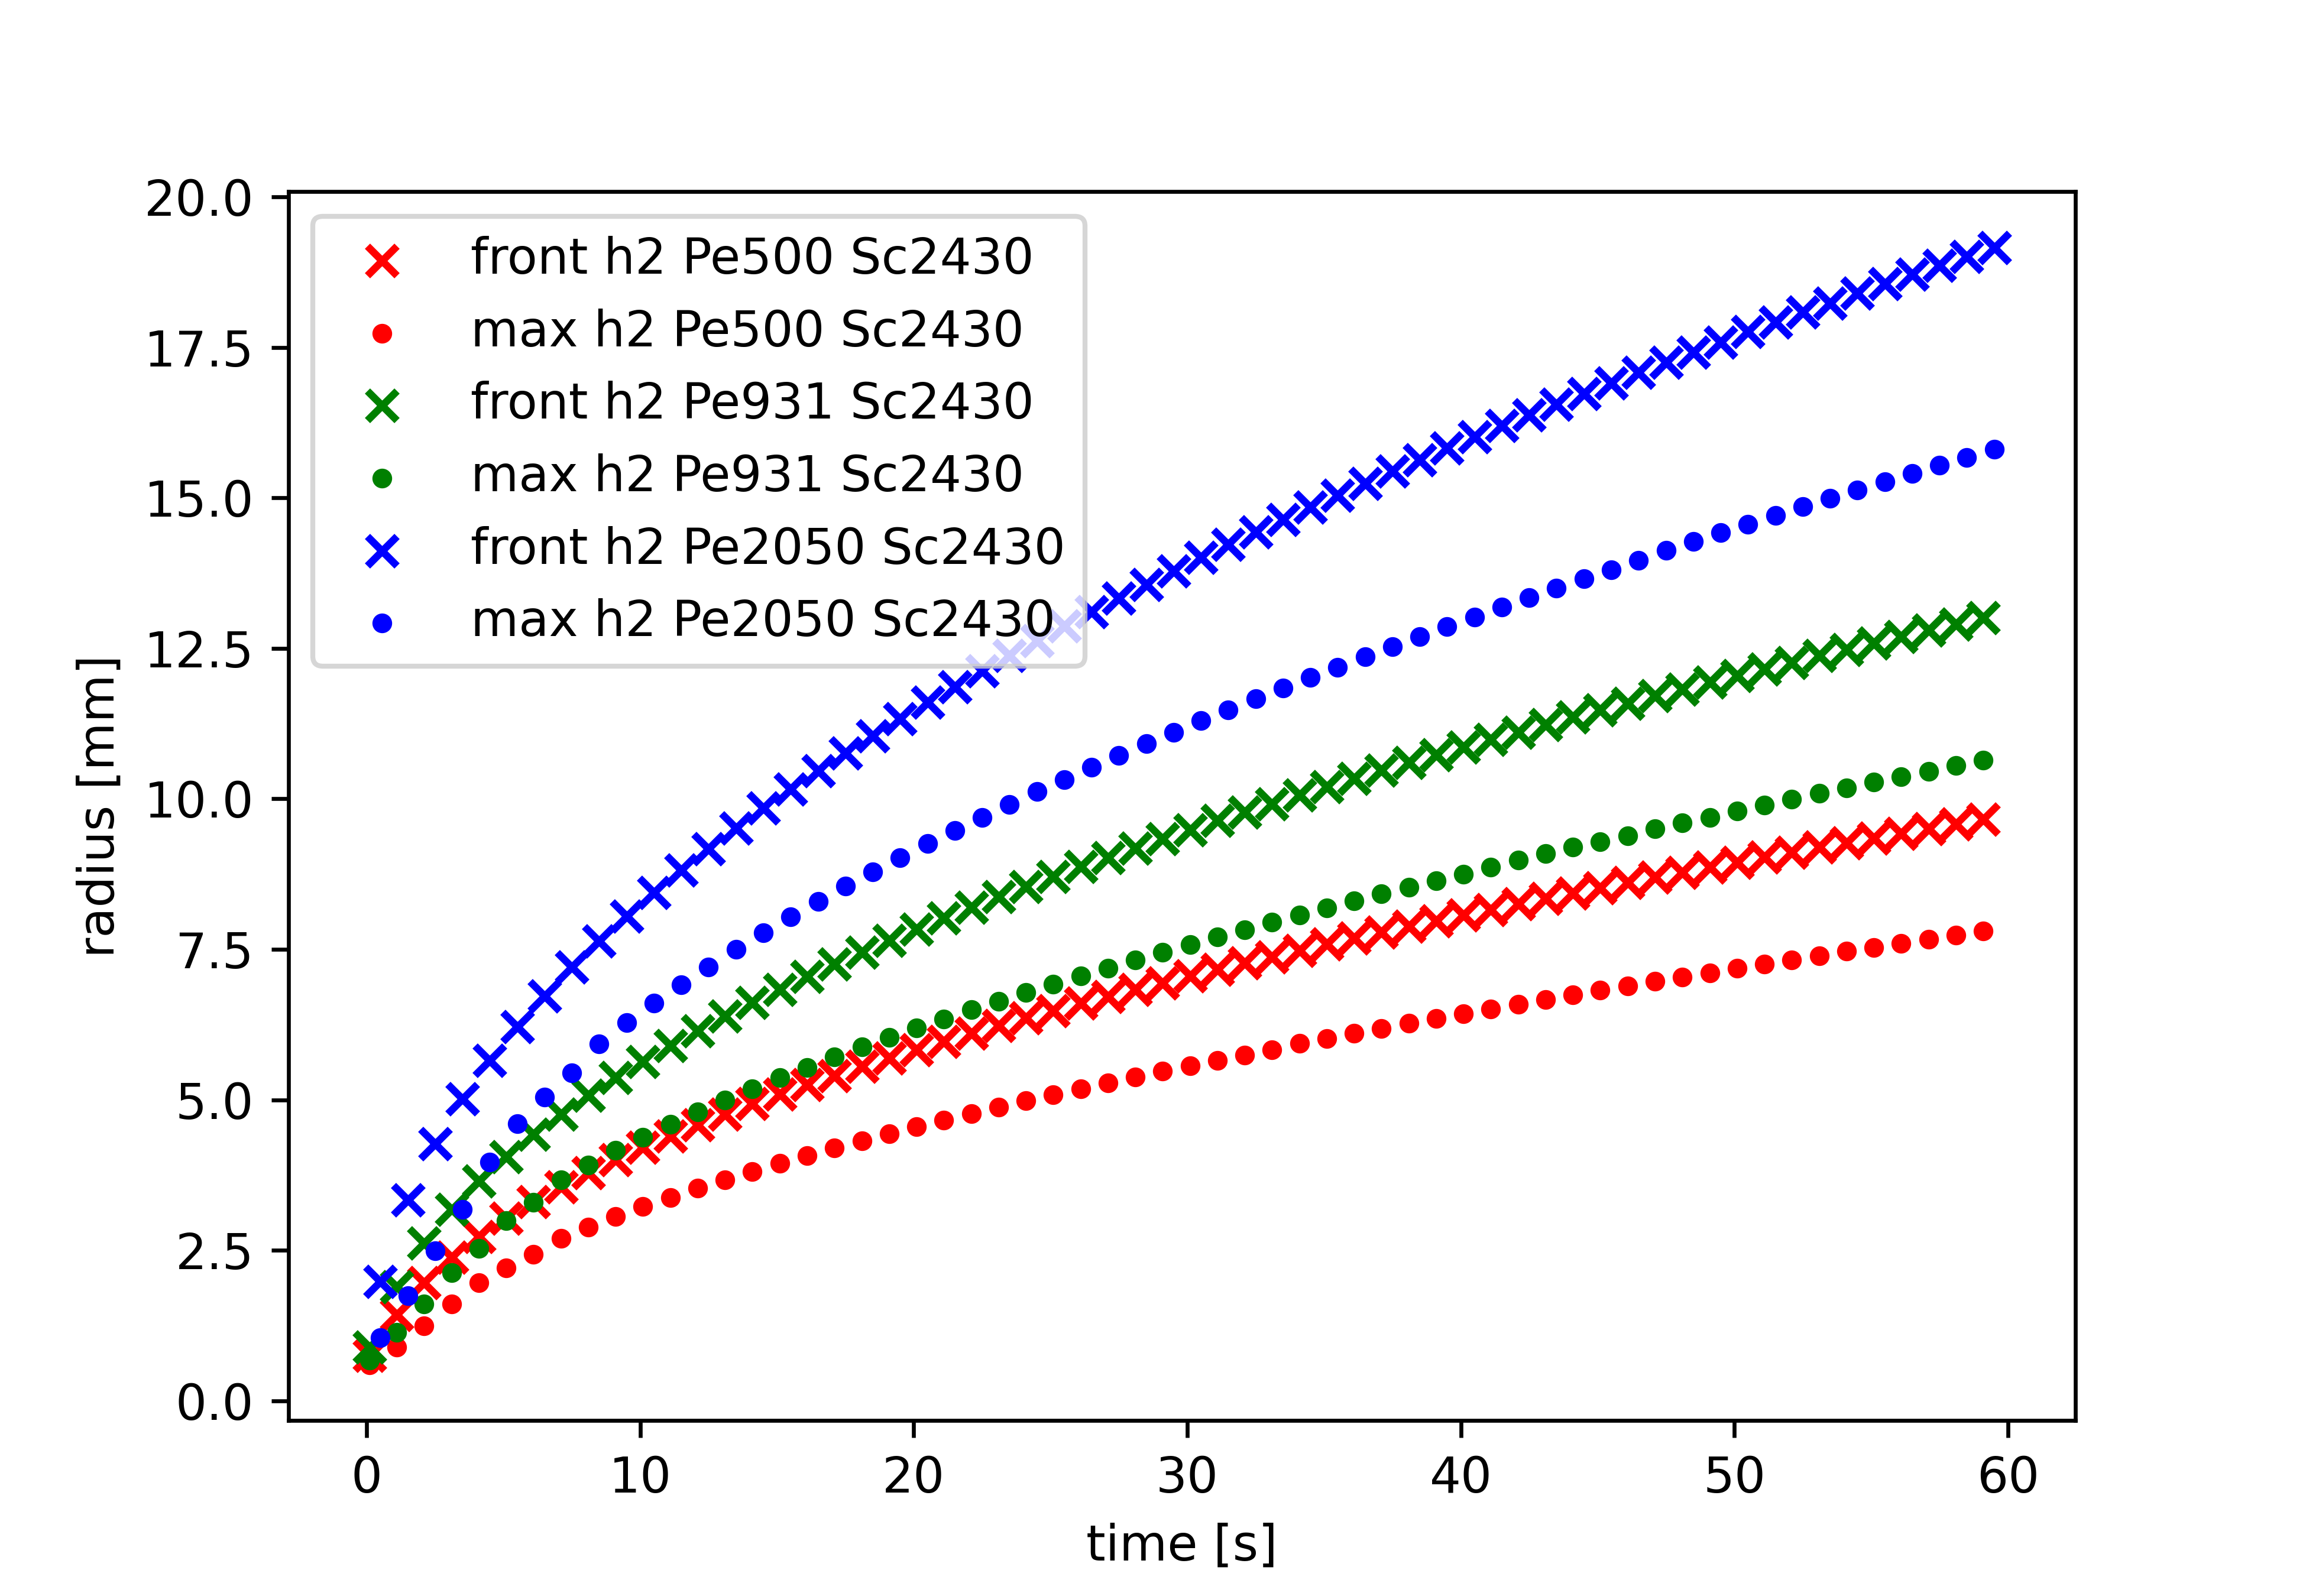
\includegraphics[width=.9\linewidth]{front_pos_h2_Sc2430}
	\caption{front positions for h 0.2mm Sc 2430\label{fig: front_pos_h2_Sc2430}}
\end{figure}

From these two graphs it can be seen that the front positions travel speed decays over time, following a behaviour close to a  square root function. The front and maximum travel faster for higher Peclet-Numbers, which can be explained by the different input velocities. The maxima positions show a similar behaviour to the front positions. 
With decreasing input velocity the difference between the fronts front and maximum positions decreases. The decrease is more significant for cases with lower Peclet-Numbers. For these cases, due to their lower inlet velocity, the distance between the front and maximum is lower. An increase in distance can be seen when comparing plots for Pecelt-Numbers of 931 with 2050.

When comparing the plots for Schmidt-Number 2430 with the one for a Schmidt-Number of 12000 it can be observed that all fronts travel nearly double the distance within the same time of 60 seconds. This can be explained mainly by the lower diffusion coefficient for the higher Schmidt-Number case. The diffusion coefficient for the lower Schmidt-Number case is $4 \text{.}11 \cdot 10^{-10} \left[ \frac{\mathrm{m^2}}{\mathrm{s}} \right]$ and the one for the higher case is $1\text{.}0 \cdot 10^{-10} \left[ \frac{\mathrm{m^2}}{\mathrm{s}} \right]$.
Since the velocity magnitude decreases very quickly for a axisymmetric reactor (see \autoref{fig: field_example}) diffusion plays a more and more significant role while the front travels through the reactor. So the diffusive fraction taking part in the front's forward travel is getting higher the further the front gets away from the inlet. The diffusion coefficient has an influence on the fronts width as well which will be look at within the following section.

\section{front widths}

The fronts widths behaviour is quite different for each reactor geometry so each one will be looked at starting with the smallest gap height of 0.2mm. The front widths for that geometry are shown in \autoref{fig: front_width_h2_Sc12000} and \autoref{fig: front_width_pos_h2_Sc2430} for each investigated Schmidt-Number.

\begin{figure}[htbp]
	\centering
	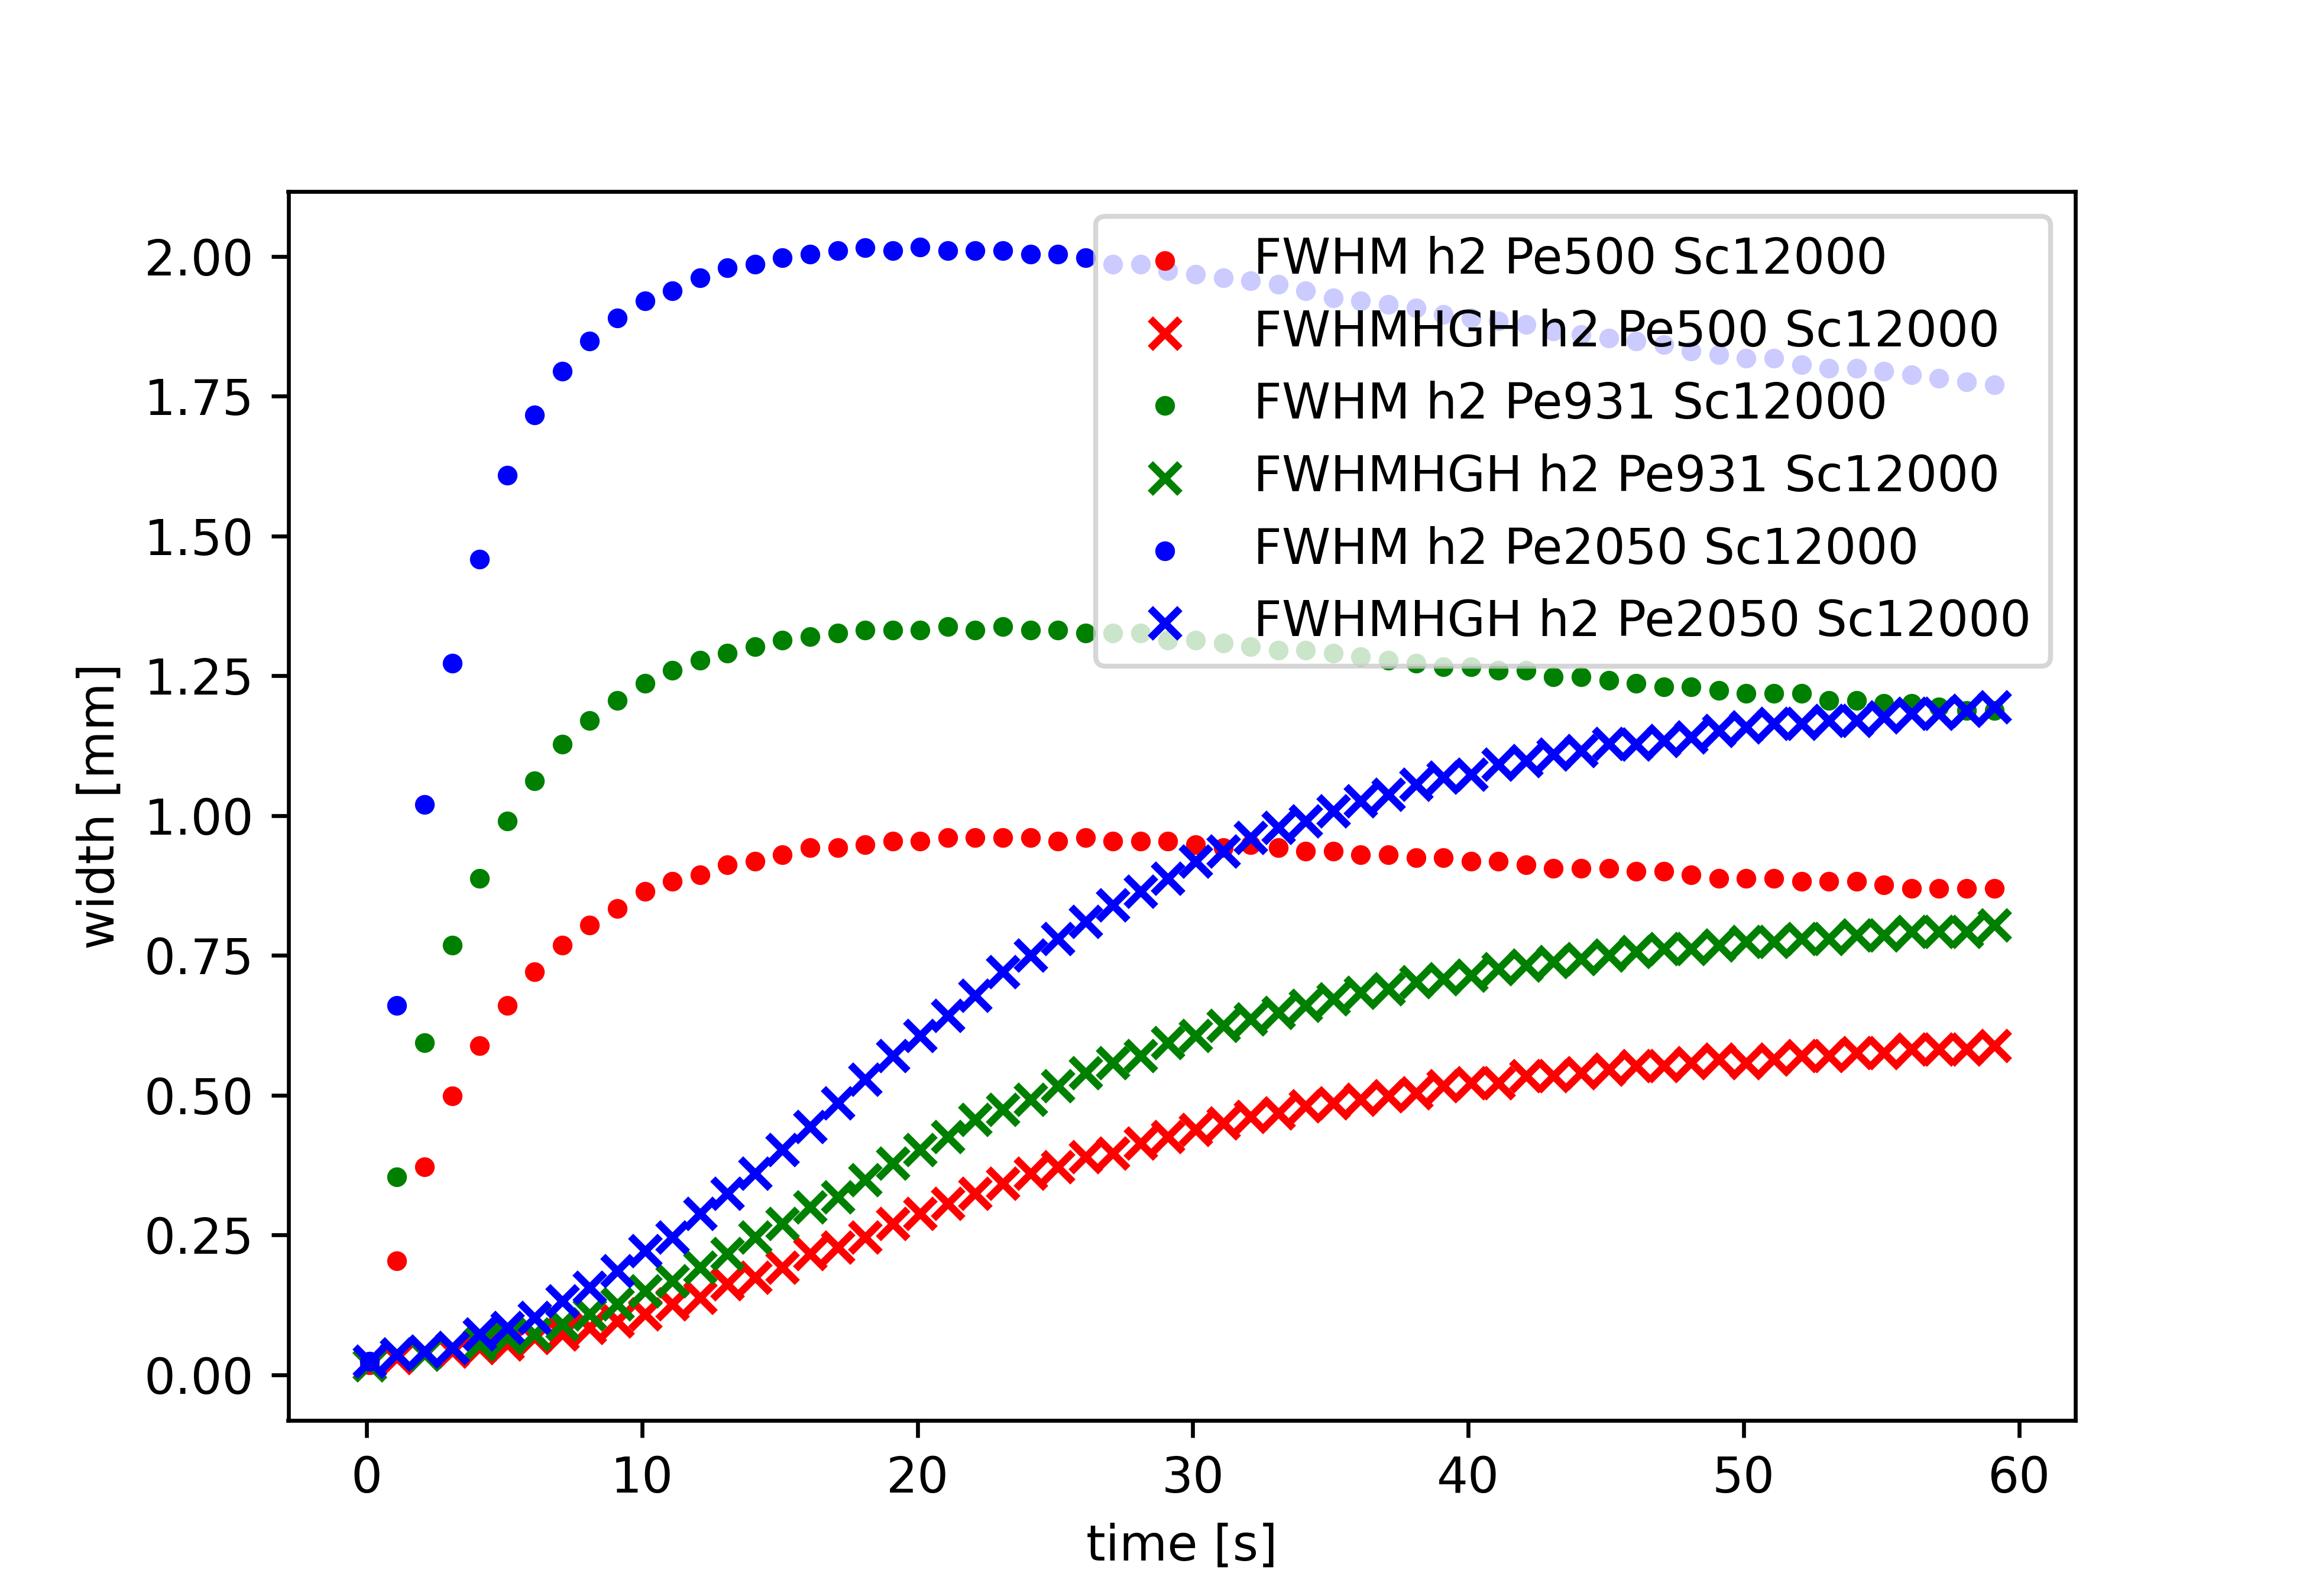
\includegraphics[width=.9\linewidth]{front_width_h2_Sc12000}
	\caption{front widths for h 0.2mm Sc 12000\label{fig: front_width_h2_Sc12000}}\bigskip
	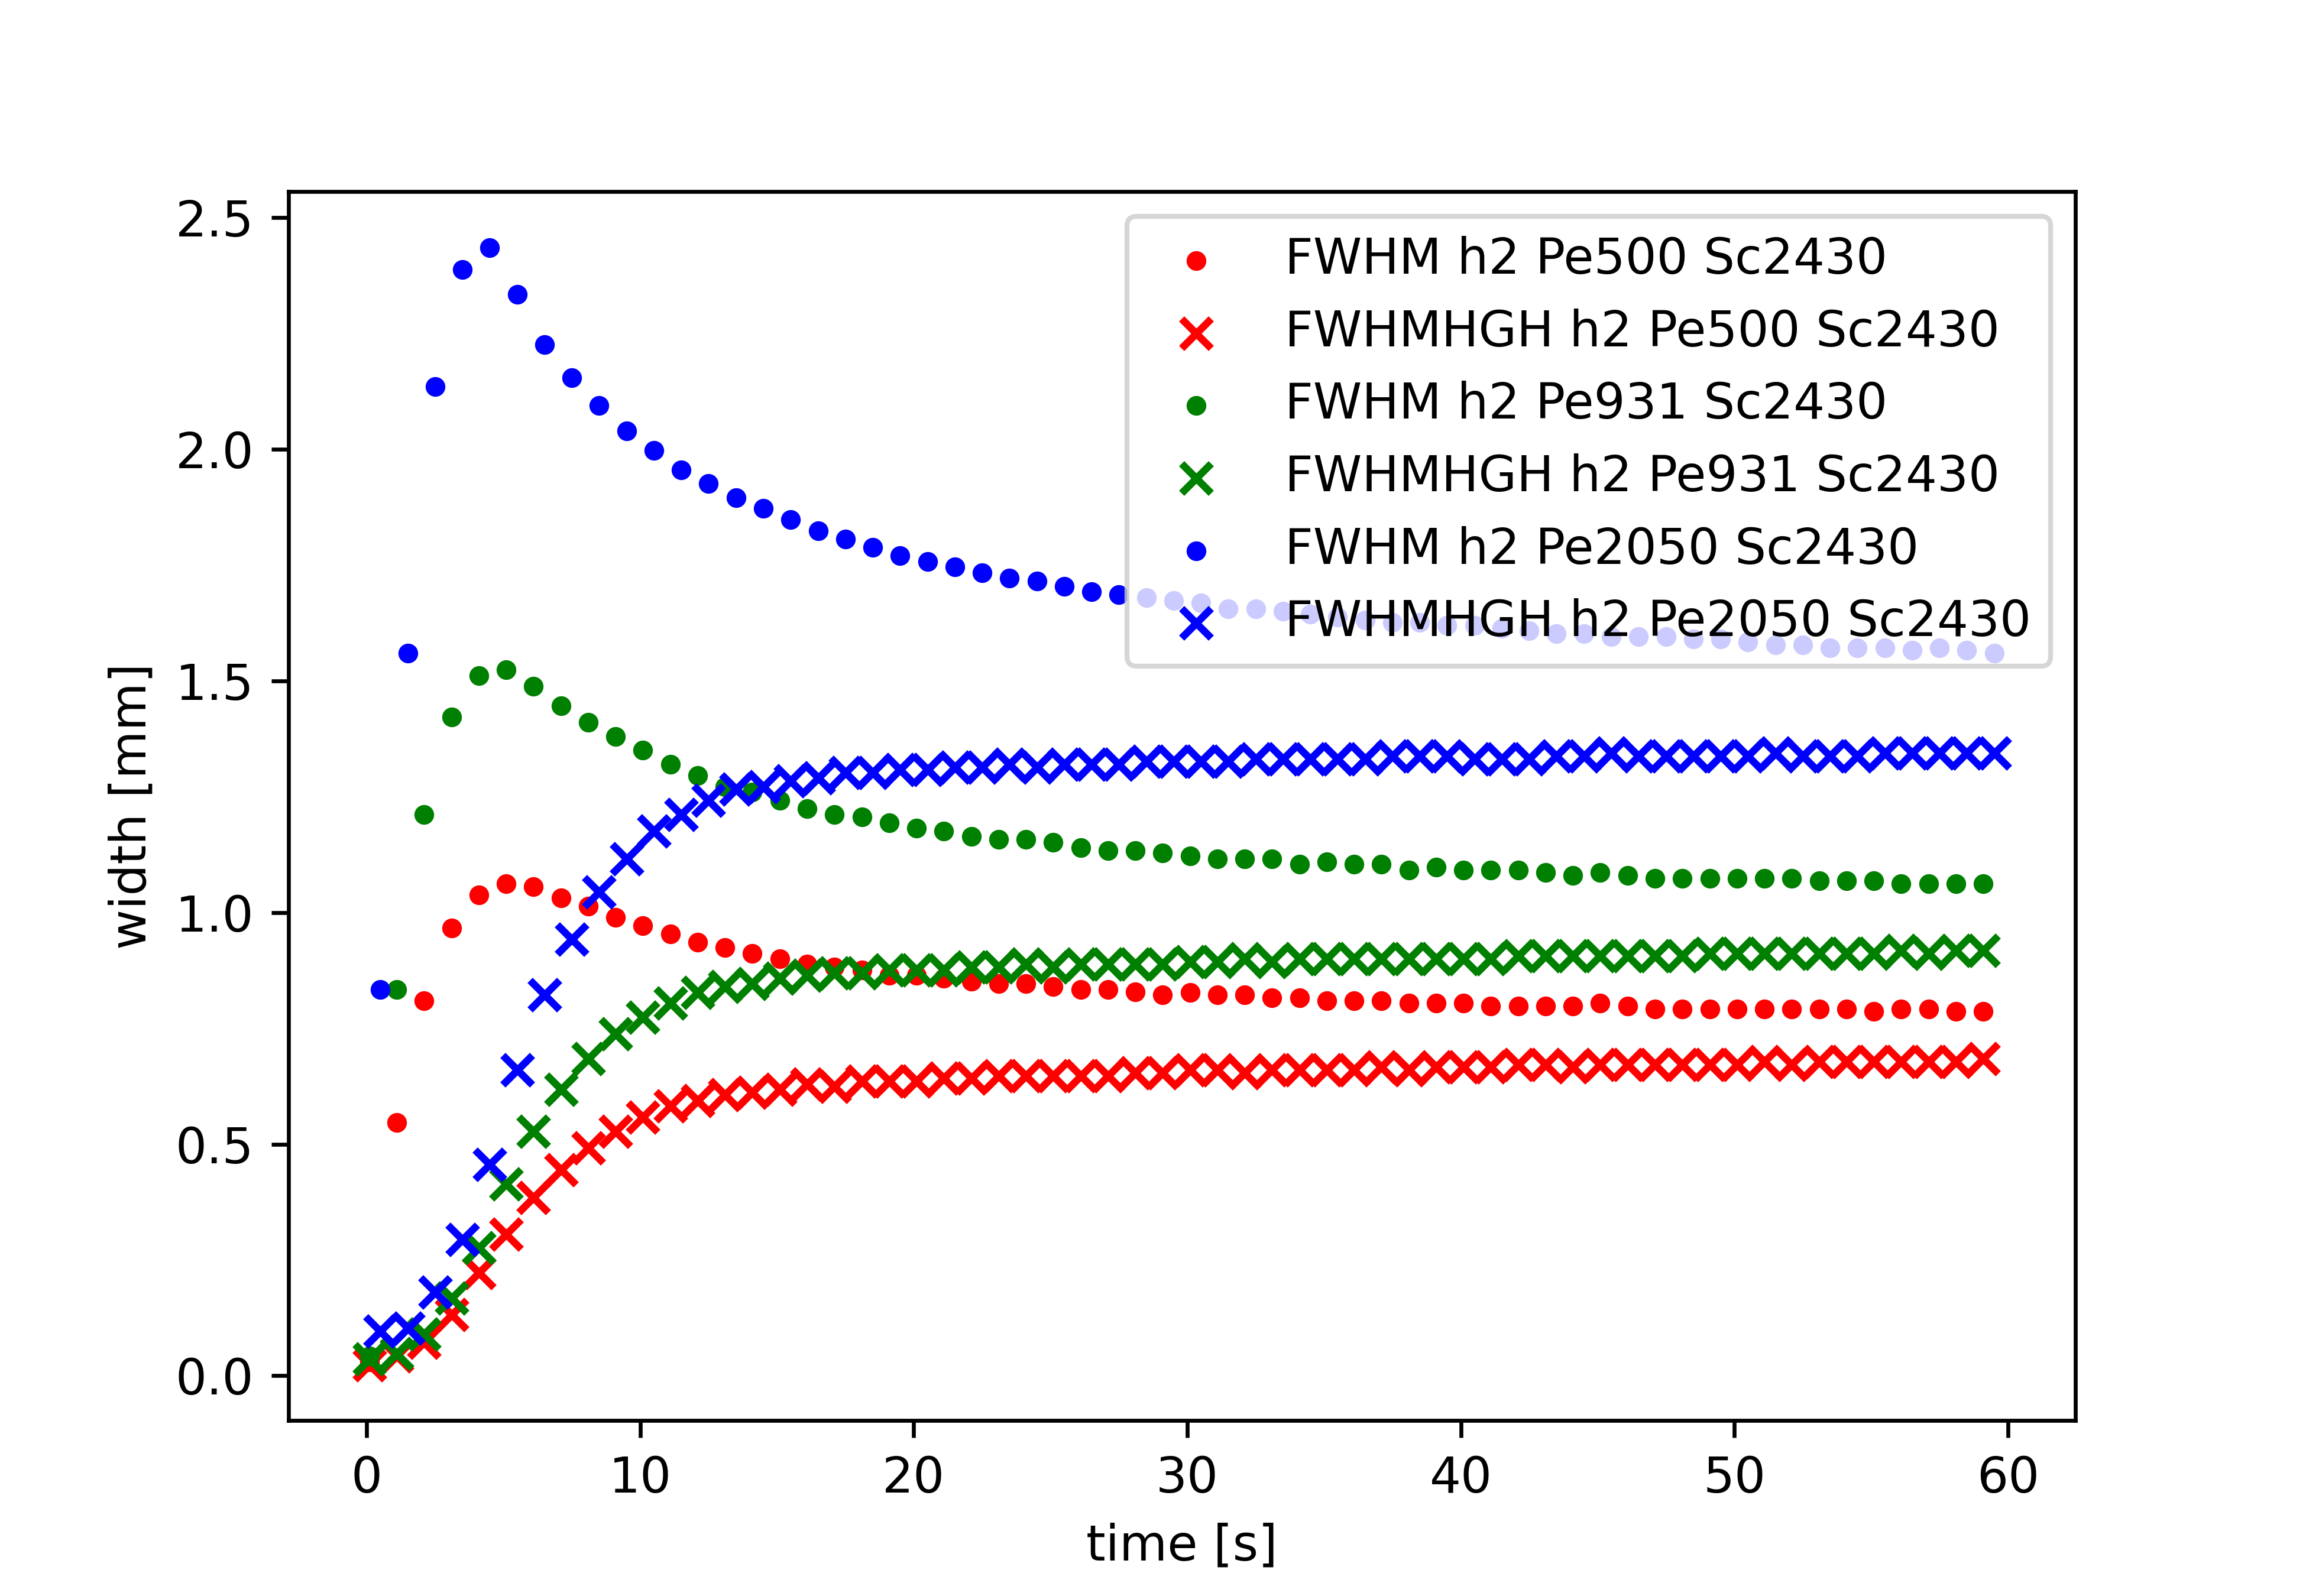
\includegraphics[width=.9\linewidth]{front_width_h2_Sc2430}
	\caption{front widths for h 0.2mm Sc 2430\label{fig: front_width_pos_h2_Sc2430}}
\end{figure}

Within these plots it can be seen that the width using the gap averaged product concentration data starts growing fast with in the first 5 seconds. After that the width's growth comes to a stop so the width reaches it's maximum value. When the maximum has been reached the width starts shrinking towards a final constant value.

The width at the reactors middle height shows a different behaviour. It's growth starts slow within the first few seconds and then starts to follow a square root like approach towards a final constant value. As already seen in the front positions the widths reach higher values for higher Peclet-Numbers. The reason for that is as already mentioned the higher input velocity for higher Peclet-Numbers. At later timestamps the width using the FWHM approach and the one calculated at the reactors middle are expected to strive towards the same value as time goes on. For these later timestamps the fronts shape evens out across the gap as visible in \autoref{fig: pos_h2_late}.
\begin{figure}[htb]
	\centering
	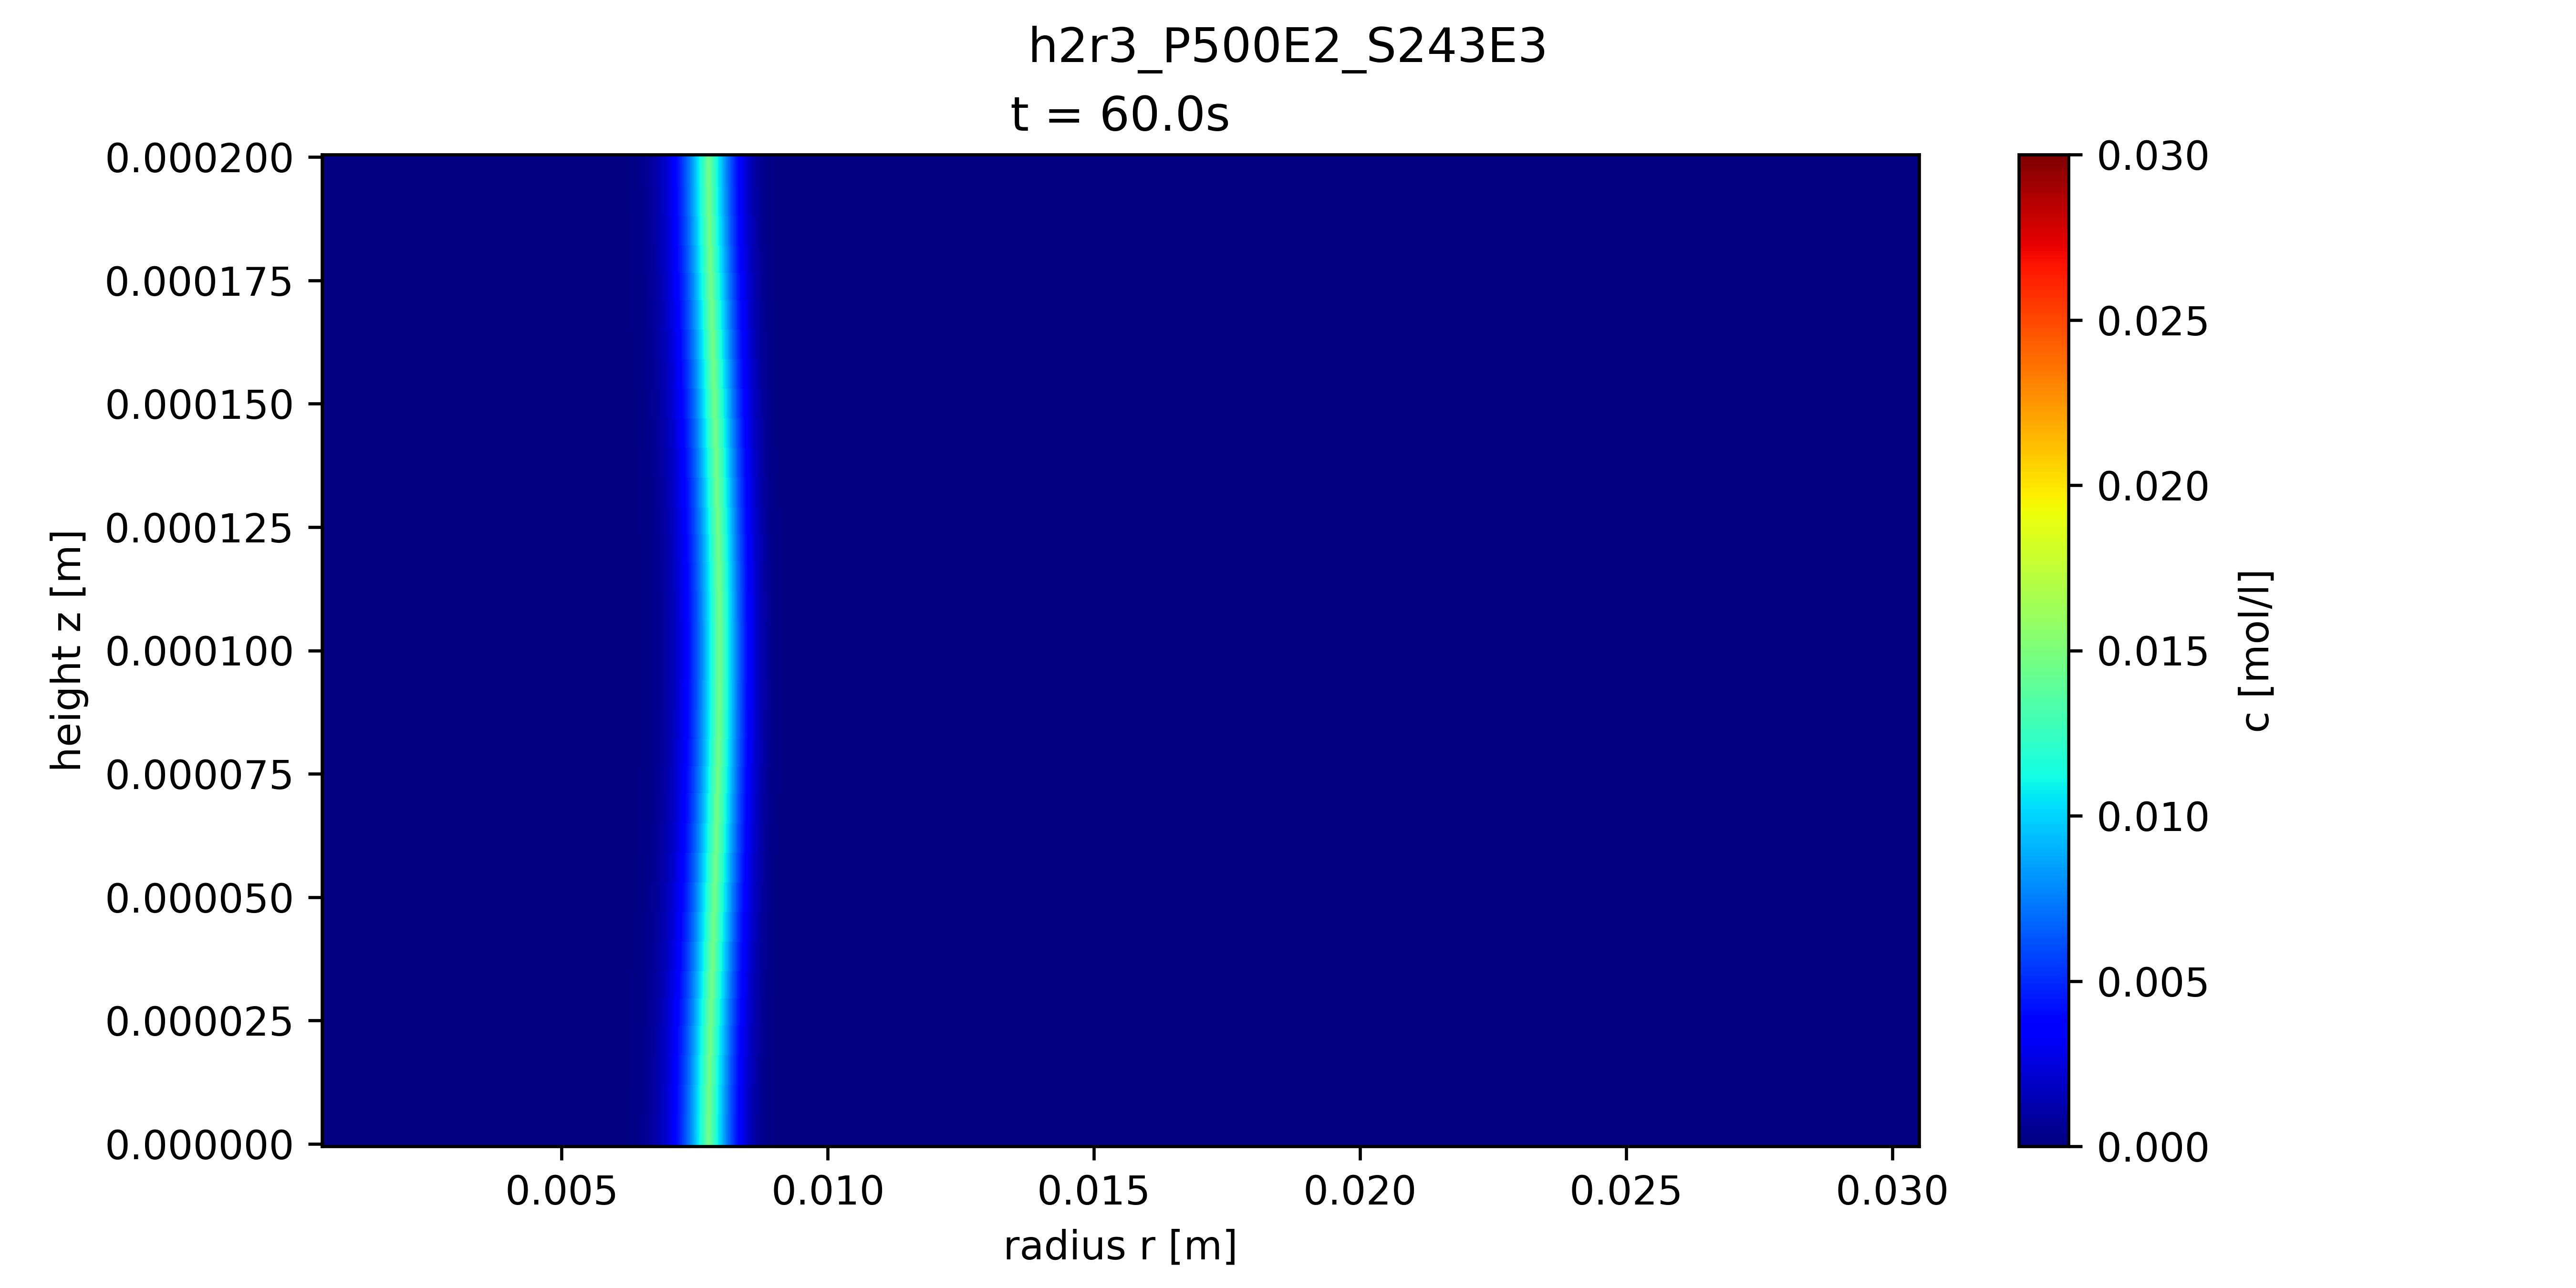
\includegraphics[width=\textwidth]{img_gif_h2r3_P500E2_S243E3_60,0 }
	\caption{front shape for Pe500 Sc2430 at 60 seconds}
	\label{fig: pos_h2_late}
\end{figure}
When the front reaches the shown shape the difference between the width using the FWHM method and the middle with decreases. The difference can only reach a value of 0 for a reactor with an infinite radius at an infinite timestamp. The effect is clearly visible even on small timescales of just 60 seconds if the Schmidt-Number and Peclet-Number are low enough.

When comparing both Schmidt-Numbers with each over it can be observed that the final width value for both widths seems to be independent of the Schmidt-Number for a gap height of 0.2mm. The results from the 0.4mm case also support this assumption. To get clearer evidence if the assumption is correct more Schmidt-Numbers need to be investigated and the simulations should be run for longer durations.
Another observation that can be made is that the time the width reaches it's maximum value and the value itself is strongly influenced by the Schmidt-Number. For the lower Schmidt-Number of 2430 a clear peak is visible for all Peclet-Numbers. This forming peak seems to be expected because as the diffusion coefficient for the case with the higher Schmidt-Number (12000) is lower than the one for the lower Schmidt-Number (2430). A lower diffusion coefficient prevents the front from spreading so the width reaches higher values. In case of the $Sc = 2430$ the width's growth happens way faster then the decay. The growth happens that quickly because new educt is pushed from the inlet into the back of the front therefore deforming it as well be shown within the 0.4mm case. The decay happens slower because the front has travelled away from the inlet so the deforming due to advection has less and less influence. The influence of advection drops proportional to $r^2$ which can be seen in the velocity field shown in \autoref{fig: field_example}. 
\newline

The results for the case with a gap height of 0.4mm show in most parts a similar behaviour compared to the case with a gap height of 0.2mm. For this geometry the FWHM width also follows a square root like approach for a high Schmidt-Number and for the lower one a peak can be observed as well. The peak is not that sharp and only visible for a Peclet-Number of 2050. The other Peclet-Numbers seem to behave similar to the cases with a gap height of 0.2mm and a Schmidt-Number of 12000. For a gap height of 0.4mm the inlet velocity seems only to be high enough for the highest Peclet-Number to form a clearly visible peak within the widths plot. The width seems to reach it's highest value in this case when the initial two different peaks merge into one which can be seen in \autoref{fig: pos_h4_peaks}.

The results for the case with a gap height of 0.4mm show a similar behaviour compared to the case with a gap height of 0.2mm. The results are shown in \autoref{fig: front_width_h4_Sc12000} and \autoref{fig: front_width_pos_h4_Sc2430}.
\begin{figure}[htbp]
	\centering
	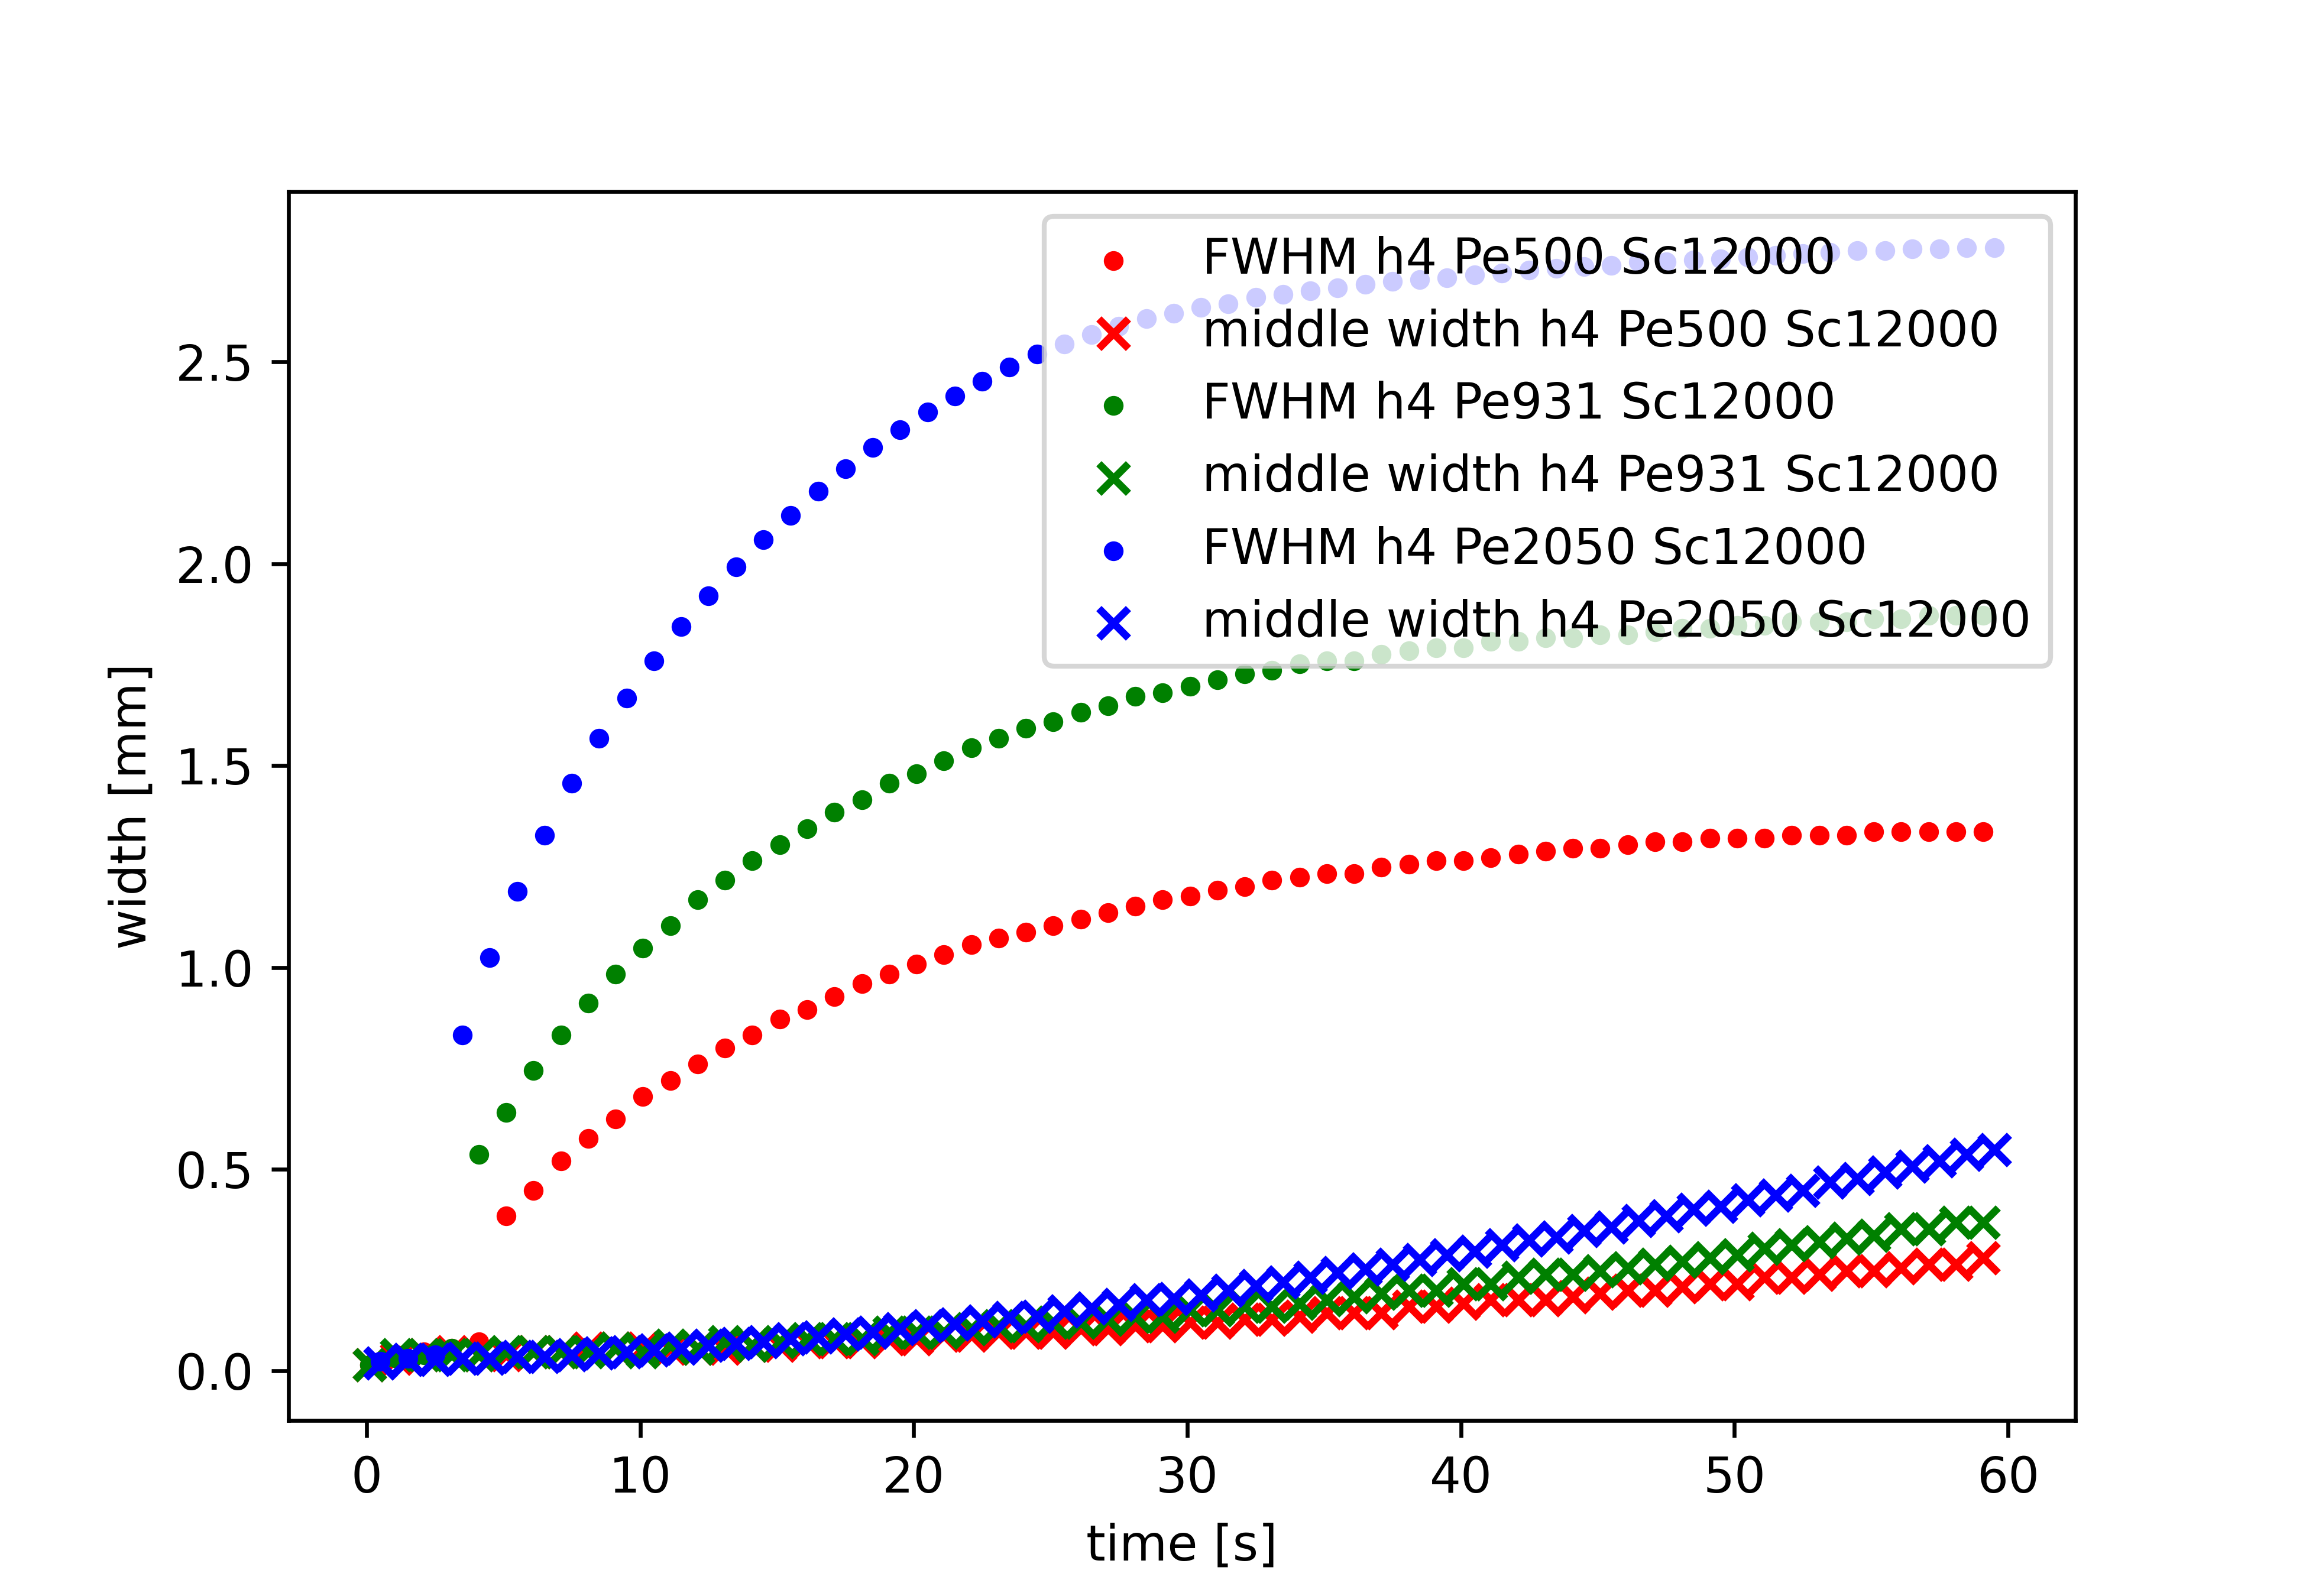
\includegraphics[width=.9\linewidth]{front_width_h4_Sc12000}
	\caption{front widths for h 0.4mm Sc 12000\label{fig: front_width_h4_Sc12000}}\bigskip
	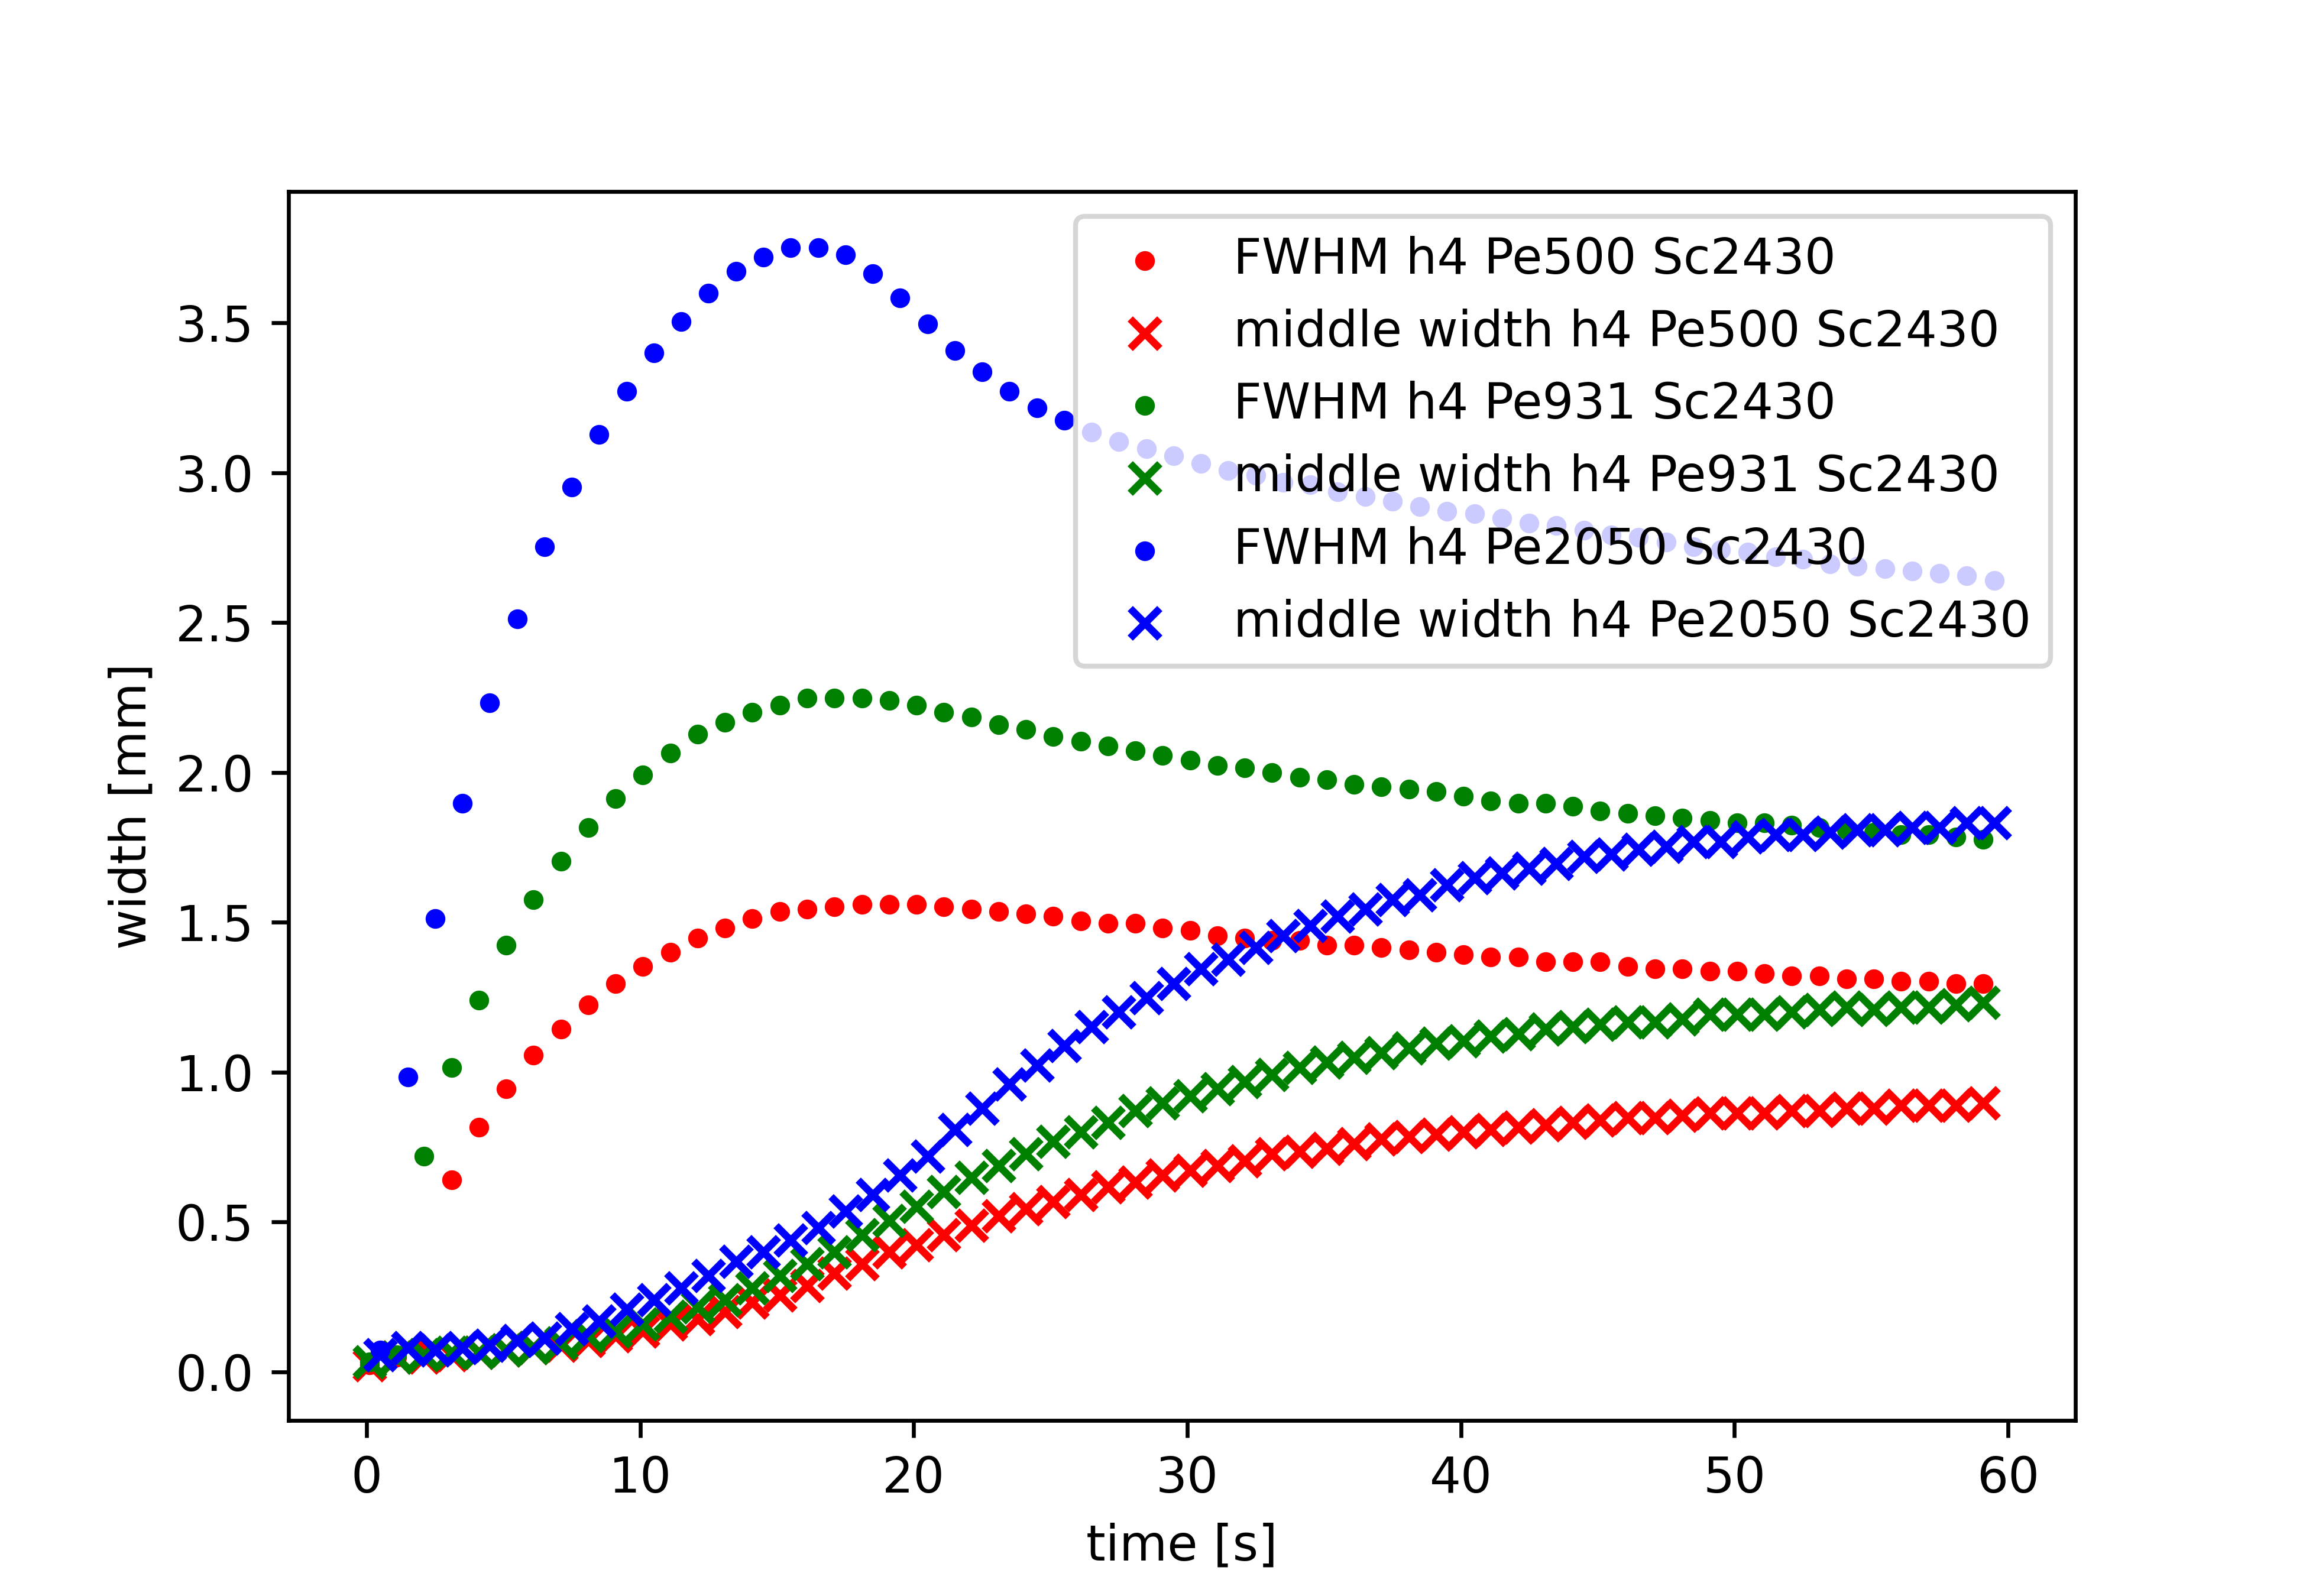
\includegraphics[width=.9\linewidth]{front_width_h4_Sc2430}
	\caption{front widths for h 0.4mm Sc 2430\label{fig: front_width_pos_h4_Sc2430}}
\end{figure}
 For this geometry the FWHM width also follows a square root like approach for a high Schmidt-Number and for the lower one a peak can be observed. The peak is not that sharp as the one observed in the 0.2mm case and only visible for a Peclet-Number of 2050. The other Peclet-Numbers seem to behave similar to the cases with a gap height of 0.2mm and a Schmidt-Number of 12000. For a gap height of 0.4mm the input velocity seems to only be high enough for the highest Peclet-Number to form a clearly visible peak within the widths plot. The width seems to reach it's highest value in this case when the initial two different peaks visible within the concentration plots merge into one which can be seen in \autoref{fig: pos_h4_peaks}. Up to a time of around 18 seconds two peaks can be distinguished within the product concentration plots. 
\begin{figure}[htb]
	\centering
	\subfloat[\centering gap averaged concentrations]{{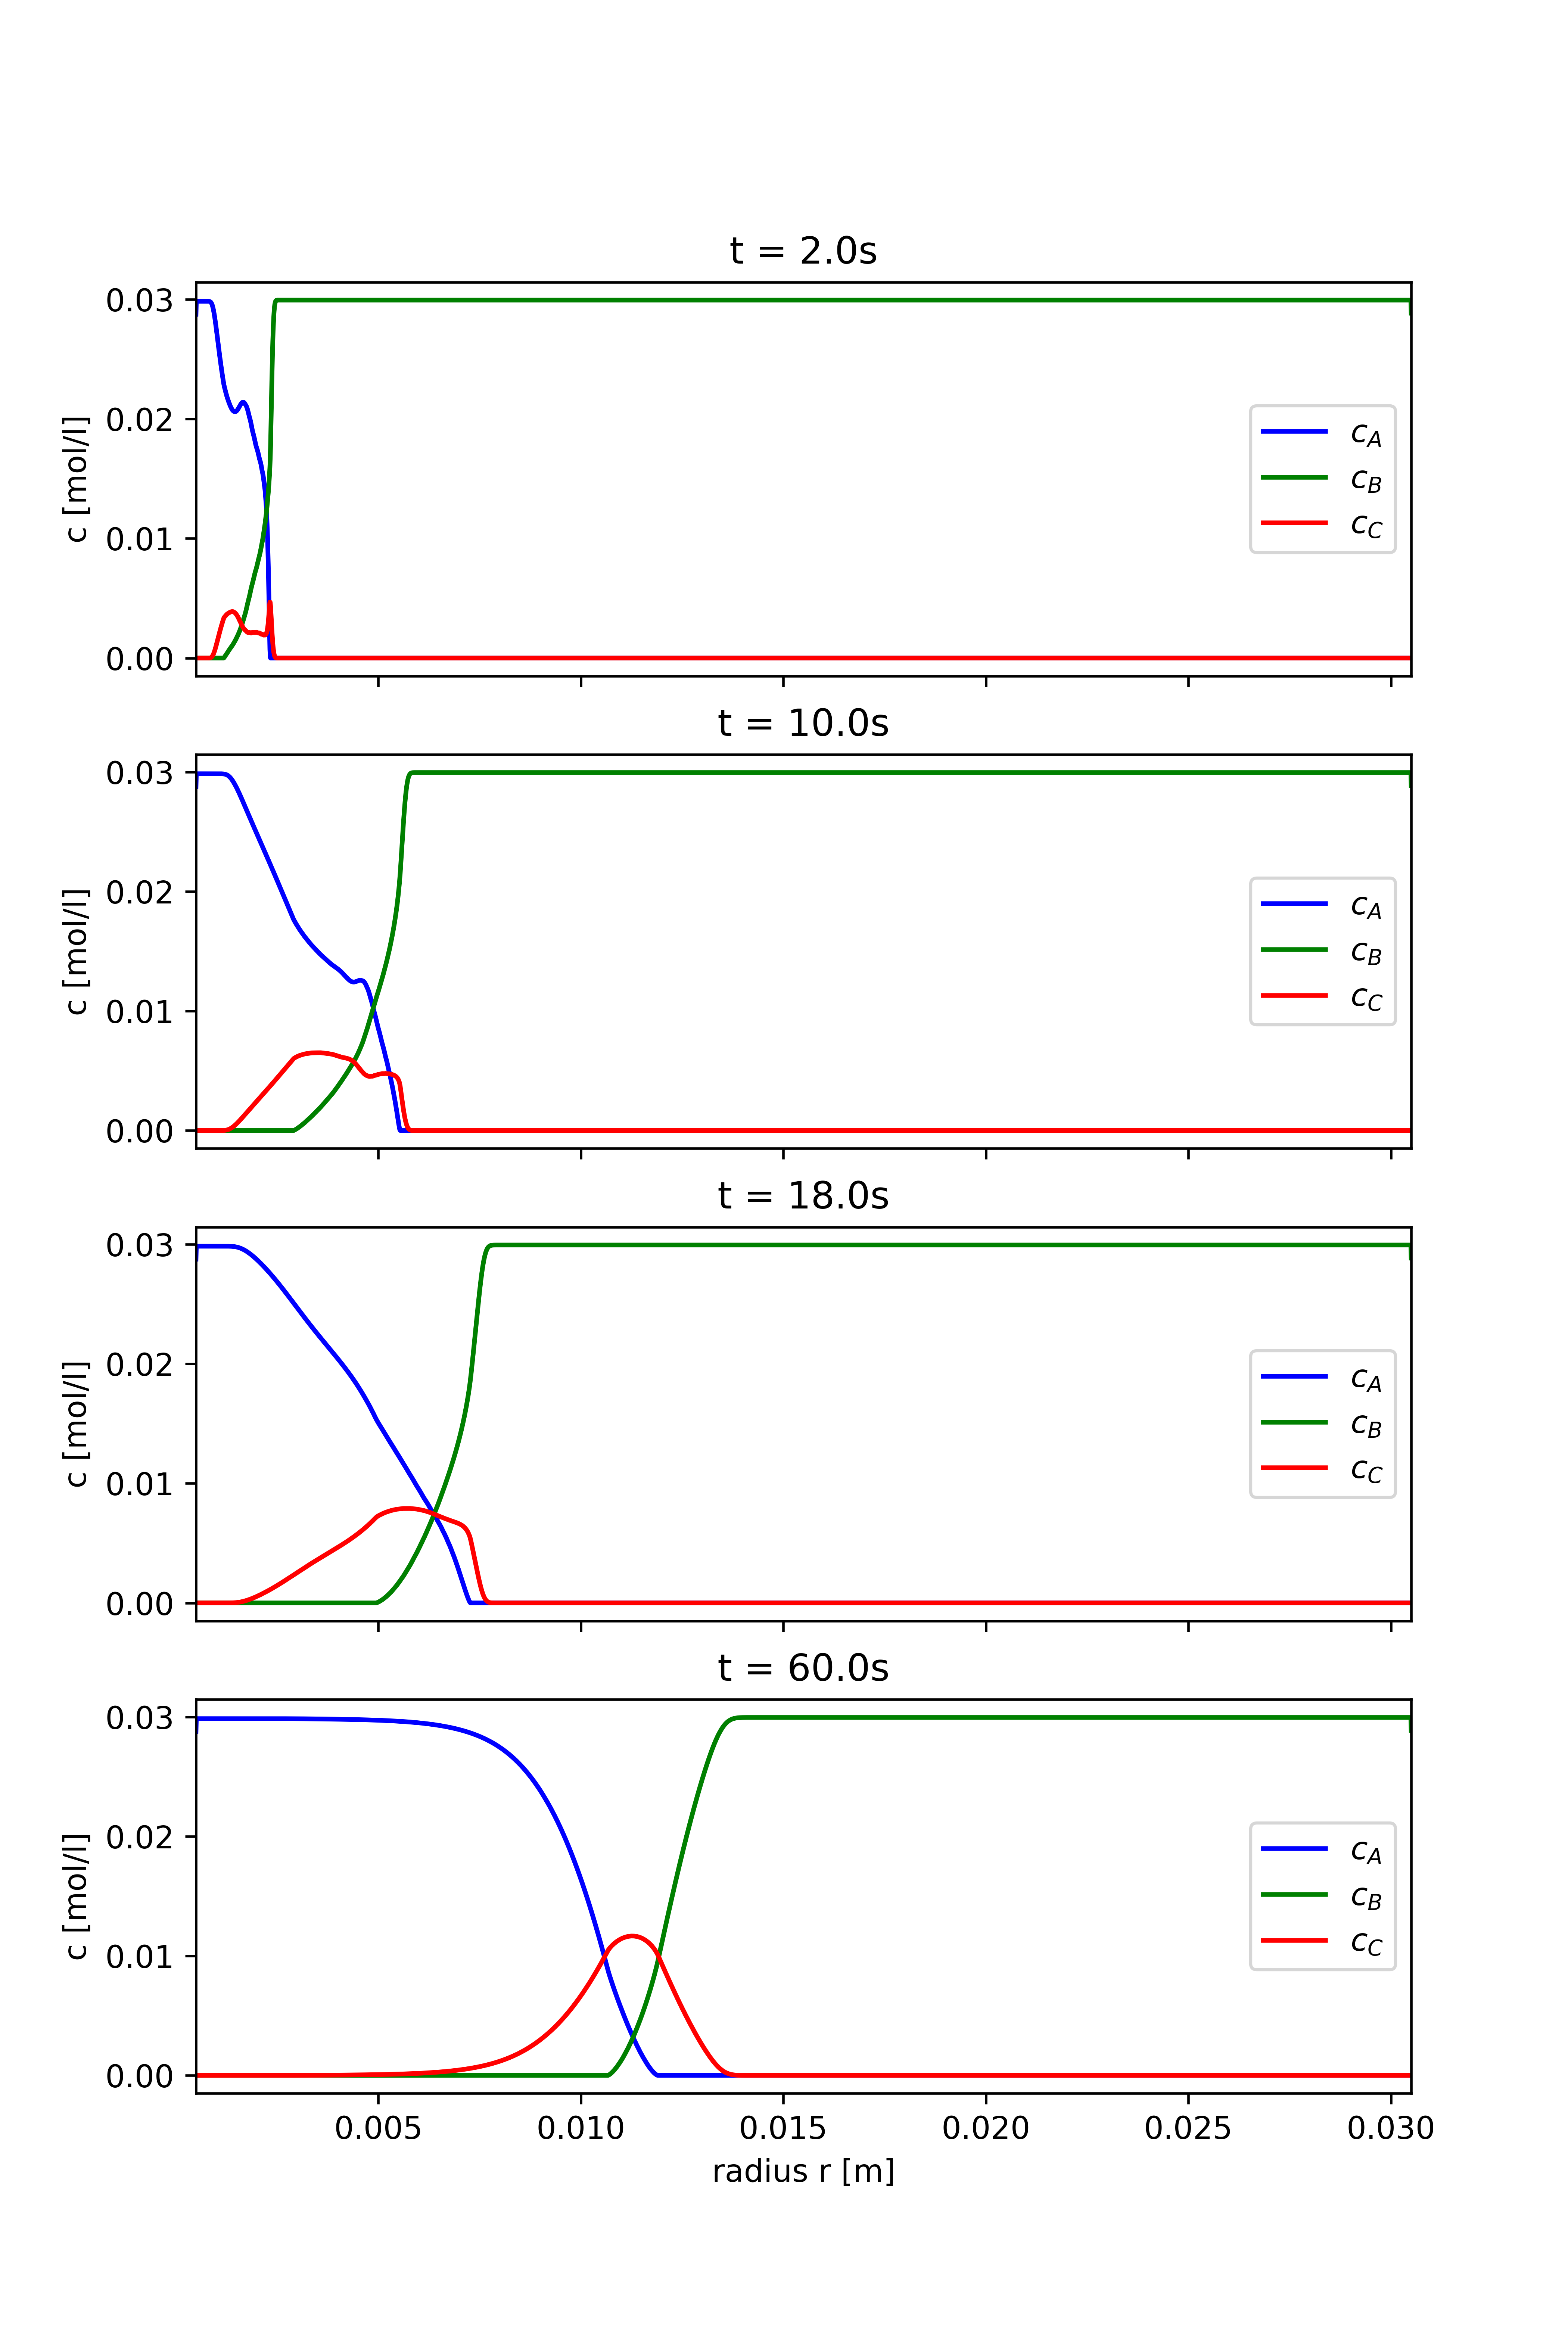
\includegraphics[angle=0, scale=0.41]{plot_h4r3_P205E3_S243E3_concentration-fluid_a_concentration-fluid_b_concentration-fluid_c} }}%
	\qquad
	\subfloat[\centering product concentration fields]{{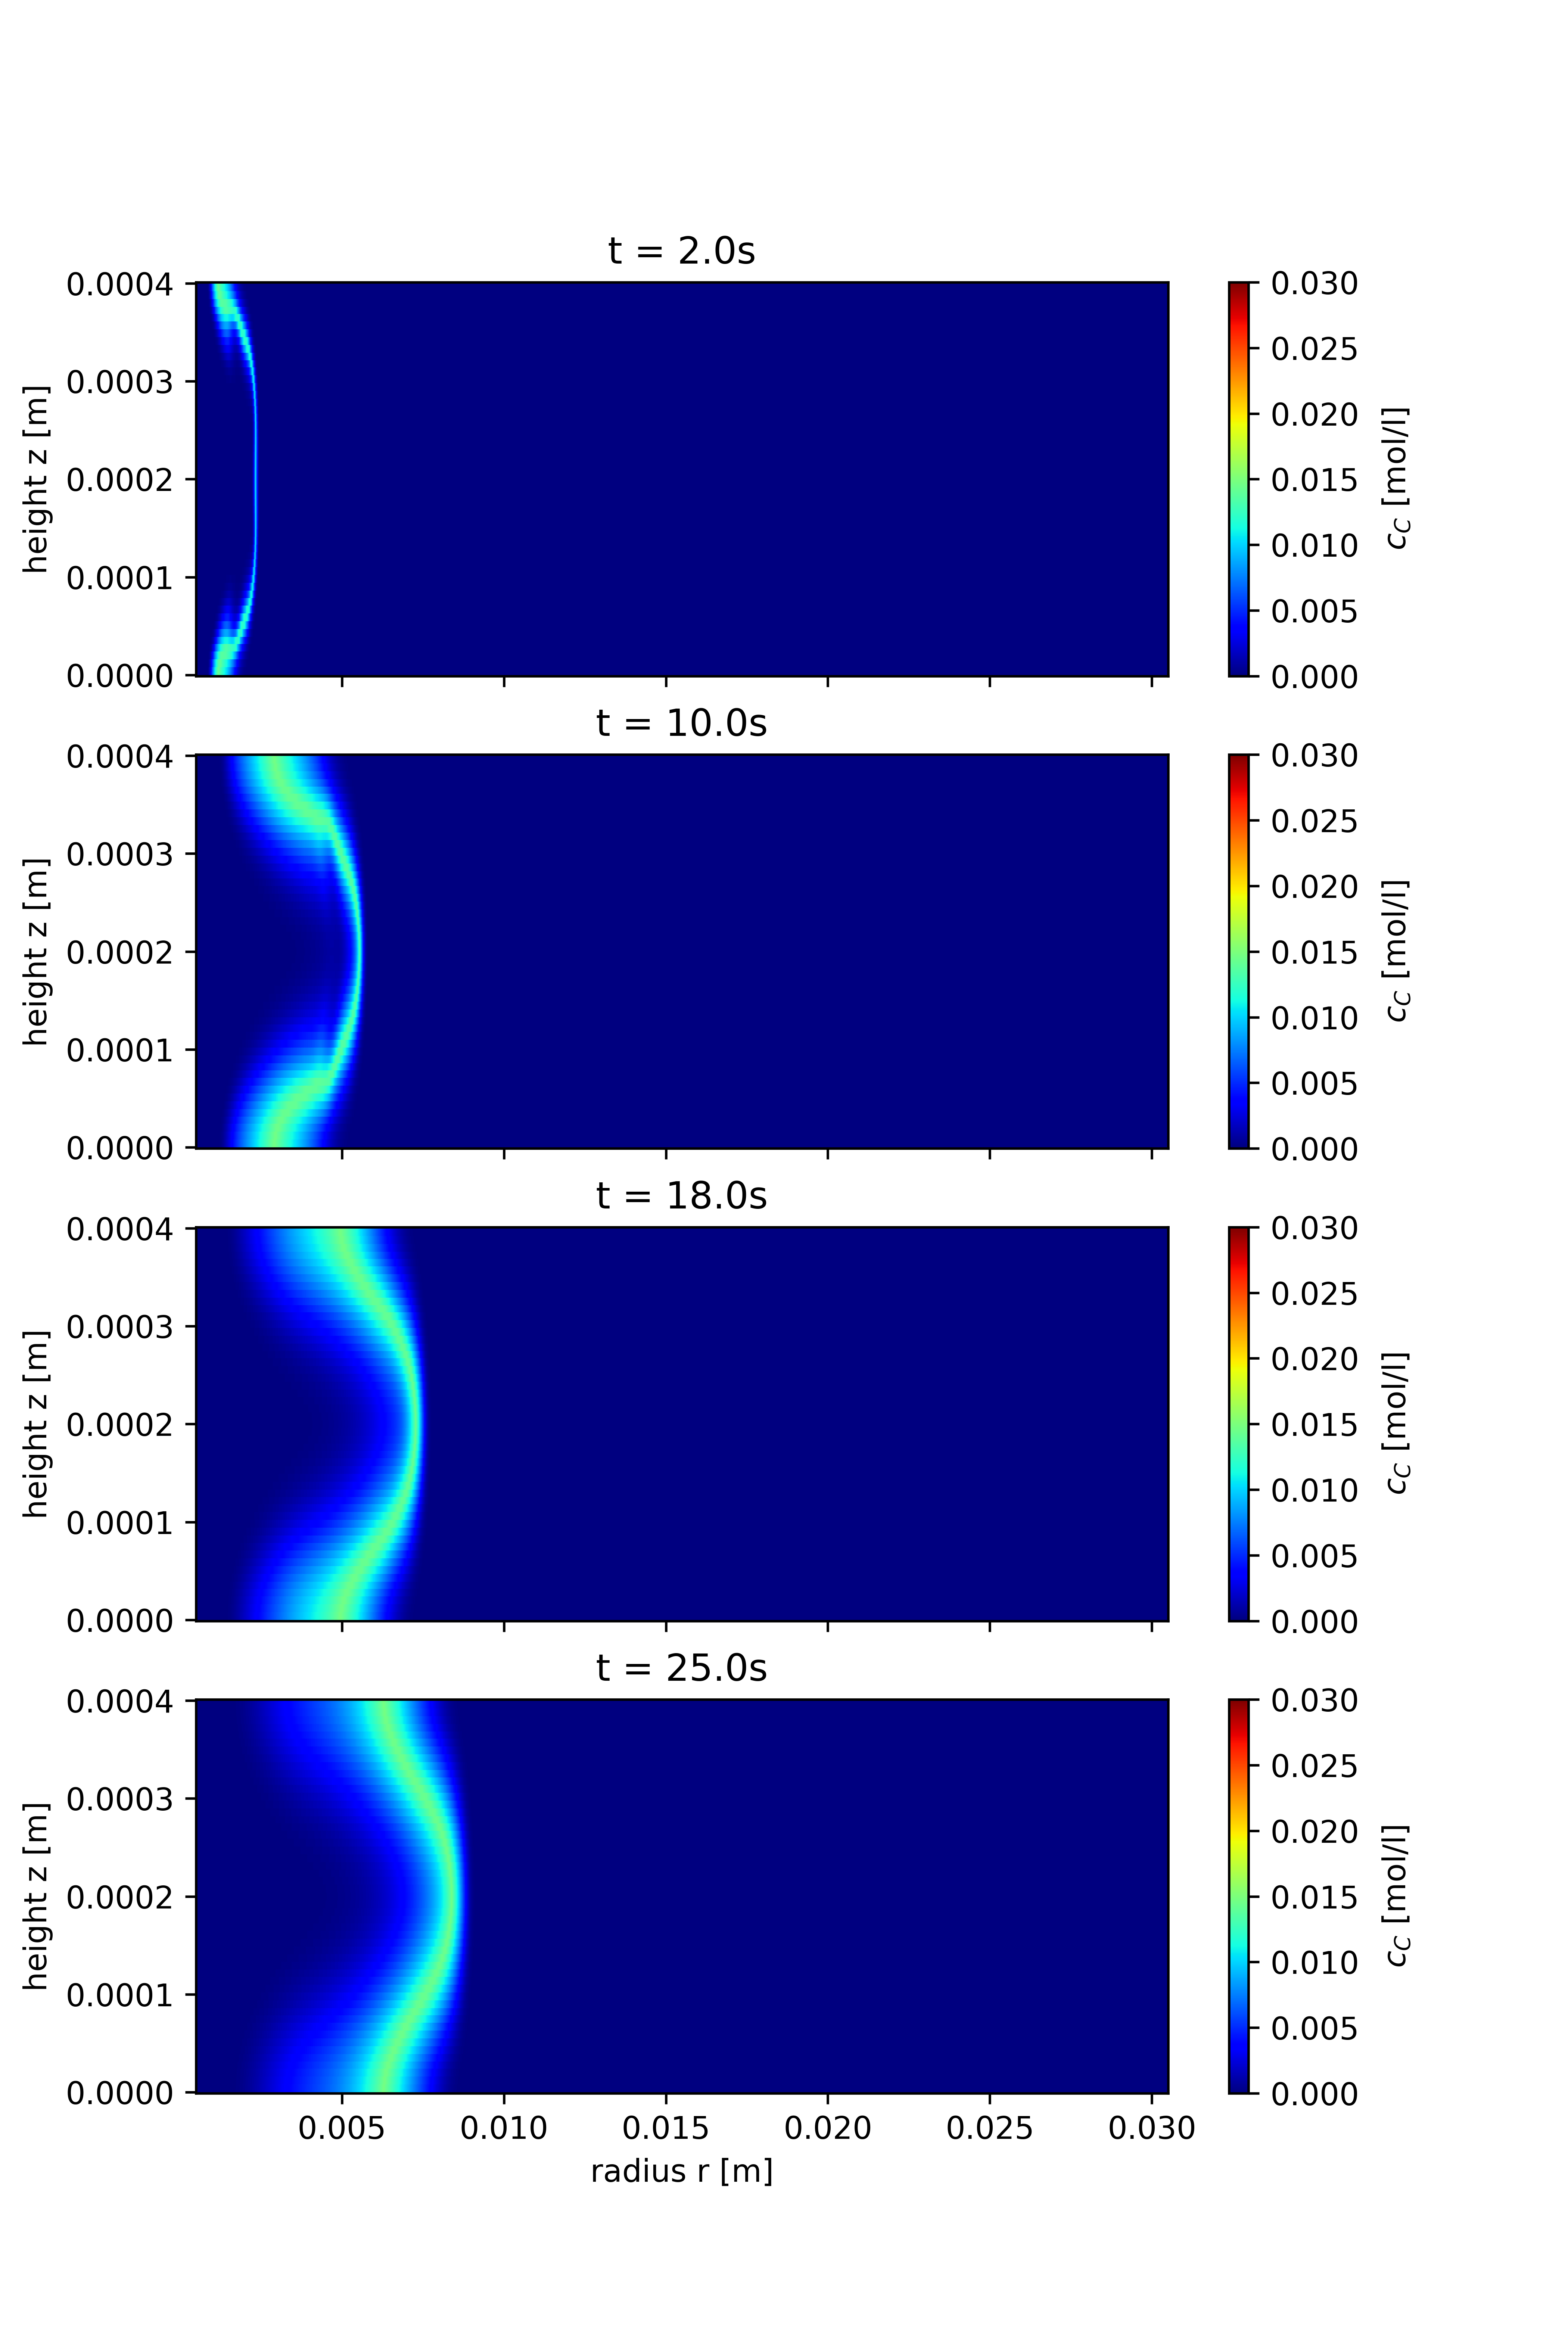
\includegraphics[angle=0, scale=0.41]{field_h4r3_P205E3_S243E3_concentration-fluid_c} }}%
	\caption{field and averaged concentration values for h0.4mm Pe2050 Sc2430}%
	\label{fig: pos_h4_peaks}%
\end{figure}
At that time the front shape has reached it's maximum curvedness. For the shown example that happens at around 18 seconds after the simulation has been started. Within the gap averaged plot it can be seen that there is a sharp increase at the fronts front and a slow decline at it's back. This decline lowers when comparing the plots for a time of 18 seconds with the one at 60 seconds. The decline can be explained by the curvedness of the front as visible in the product concentration fields plot.
\newline

For the case with a gap height of 0.6mm the width's behaviour seems to change quite significantly compared to the 0.4mm case. For the Schmidt-Number of 12000 the general form of the FWHM curves seems to match the ones from the previous discussed cases.
\begin{figure}[htbp]
	\centering
	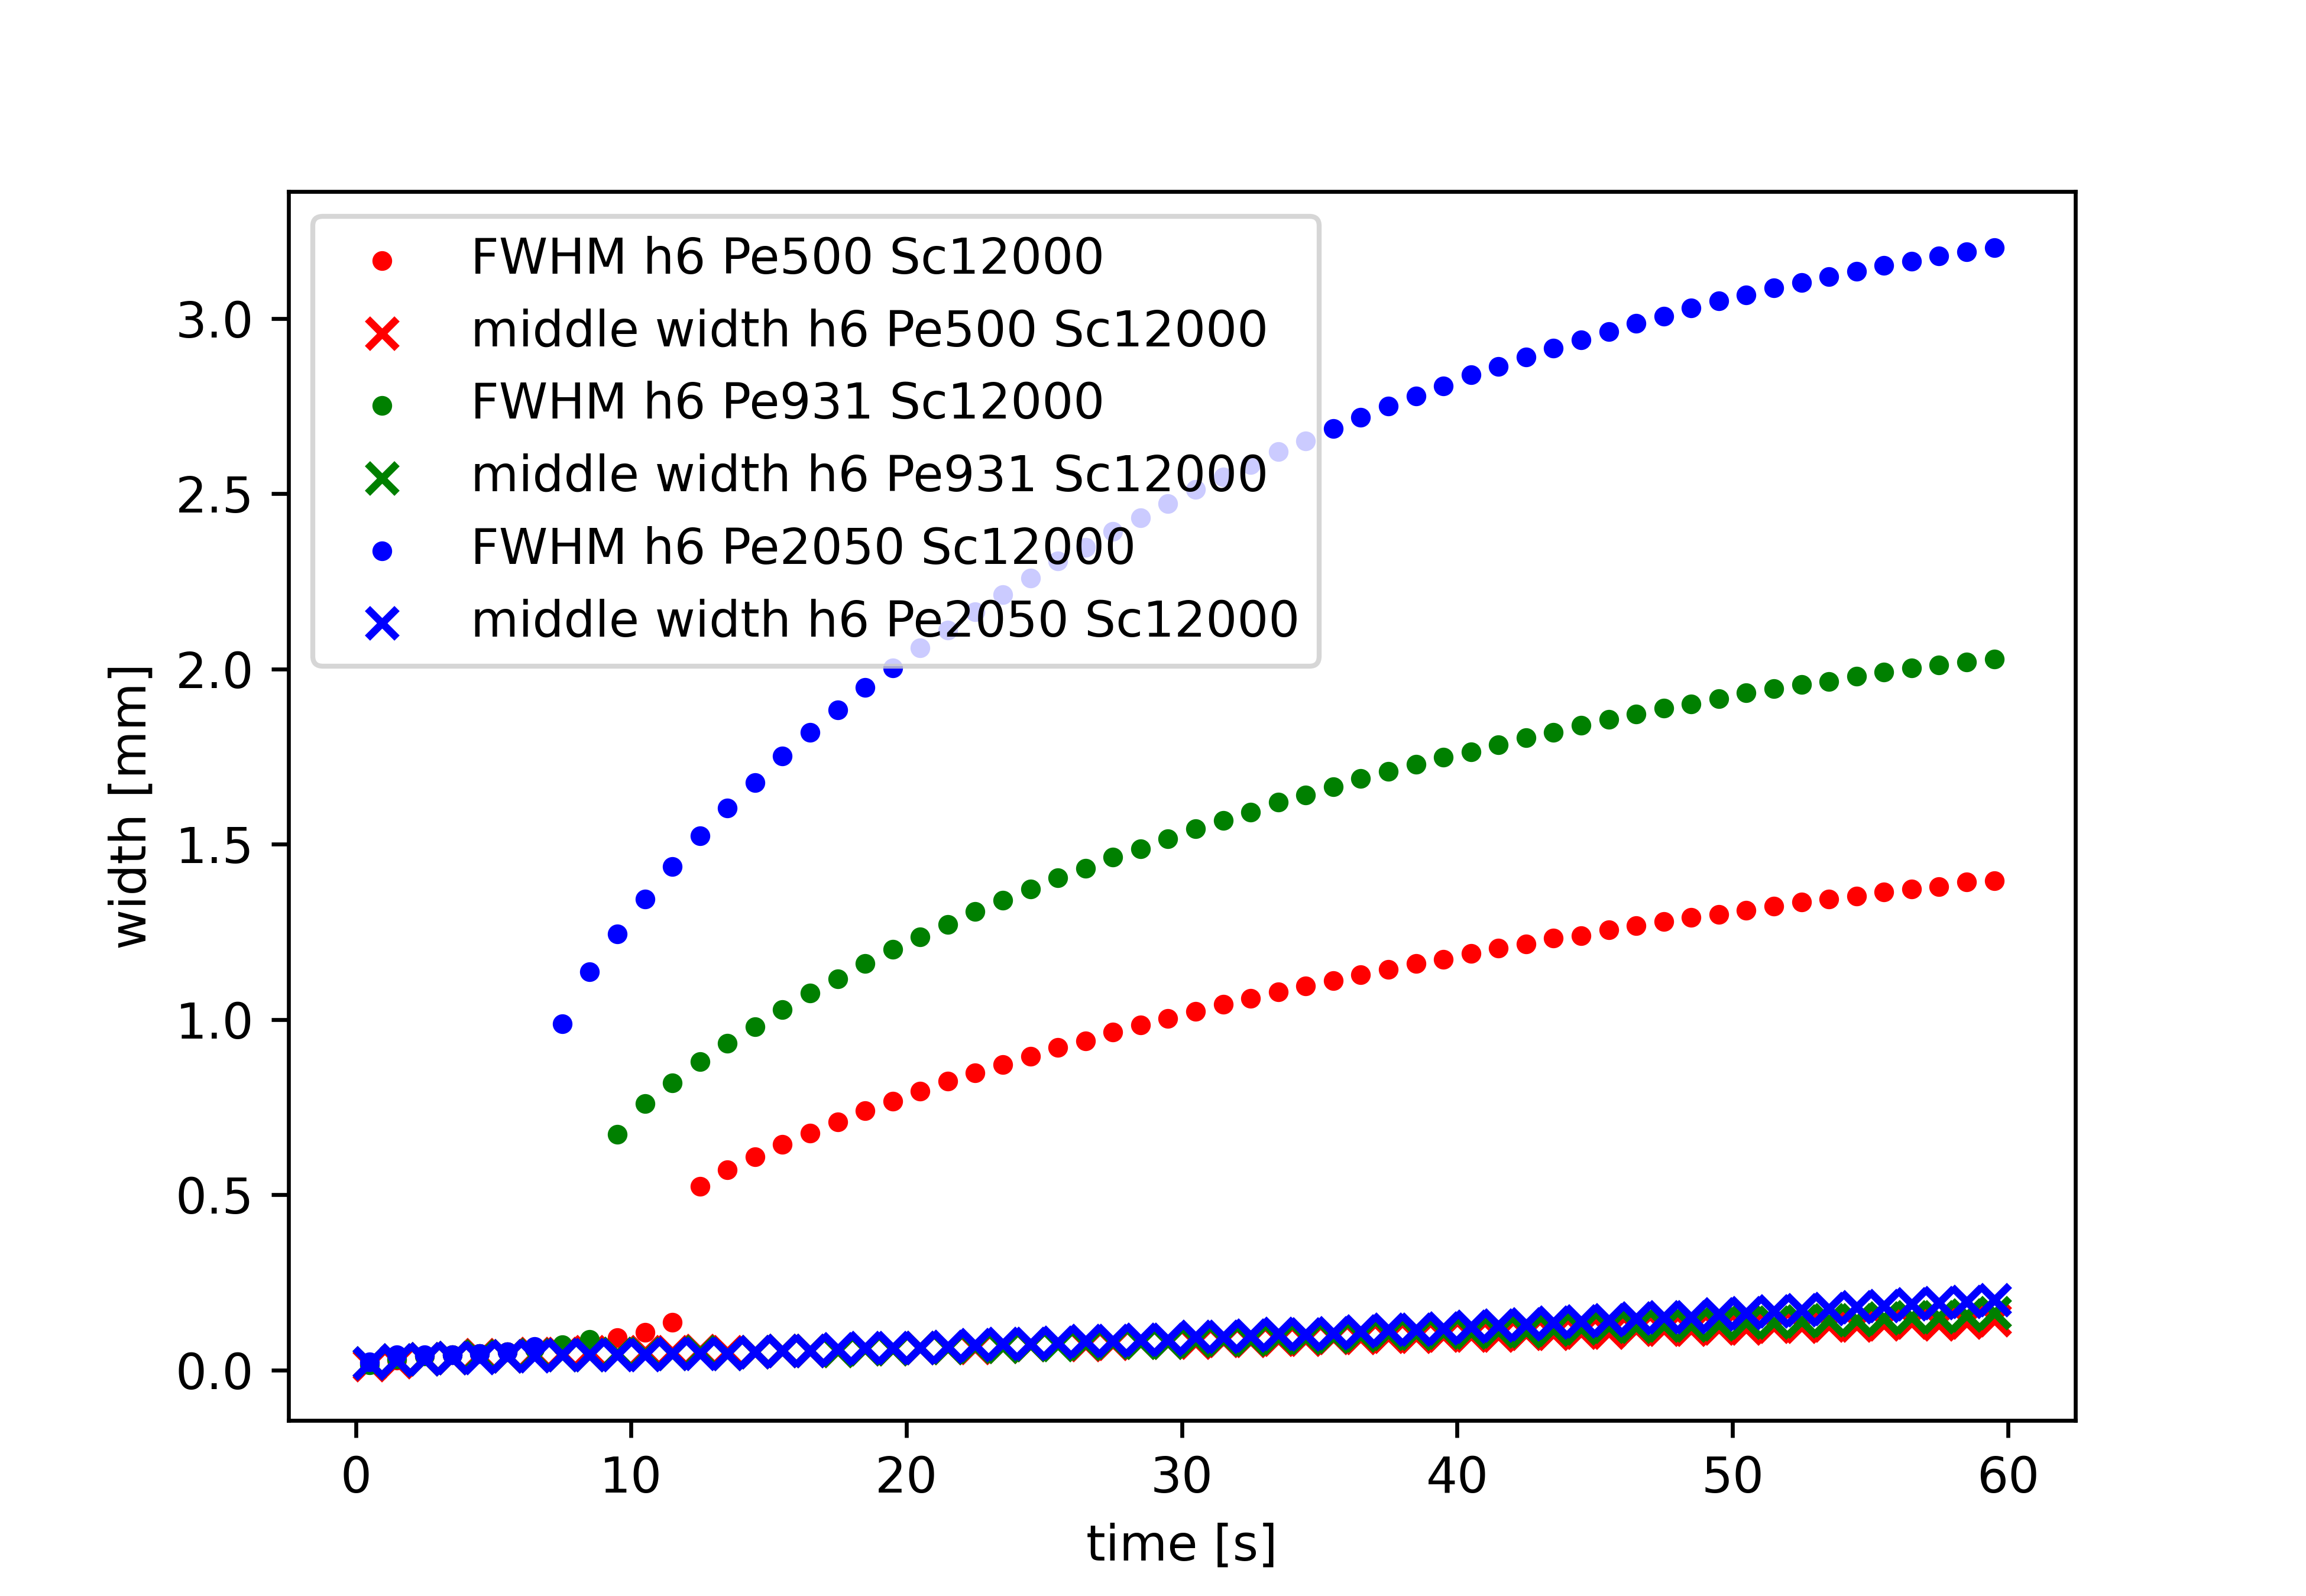
\includegraphics[width=.9\linewidth]{front_width_h6_Sc12000}
	\caption{front widths for h 0.6mm Sc 12000\label{fig: front_width_h6_Sc12000}}\bigskip
	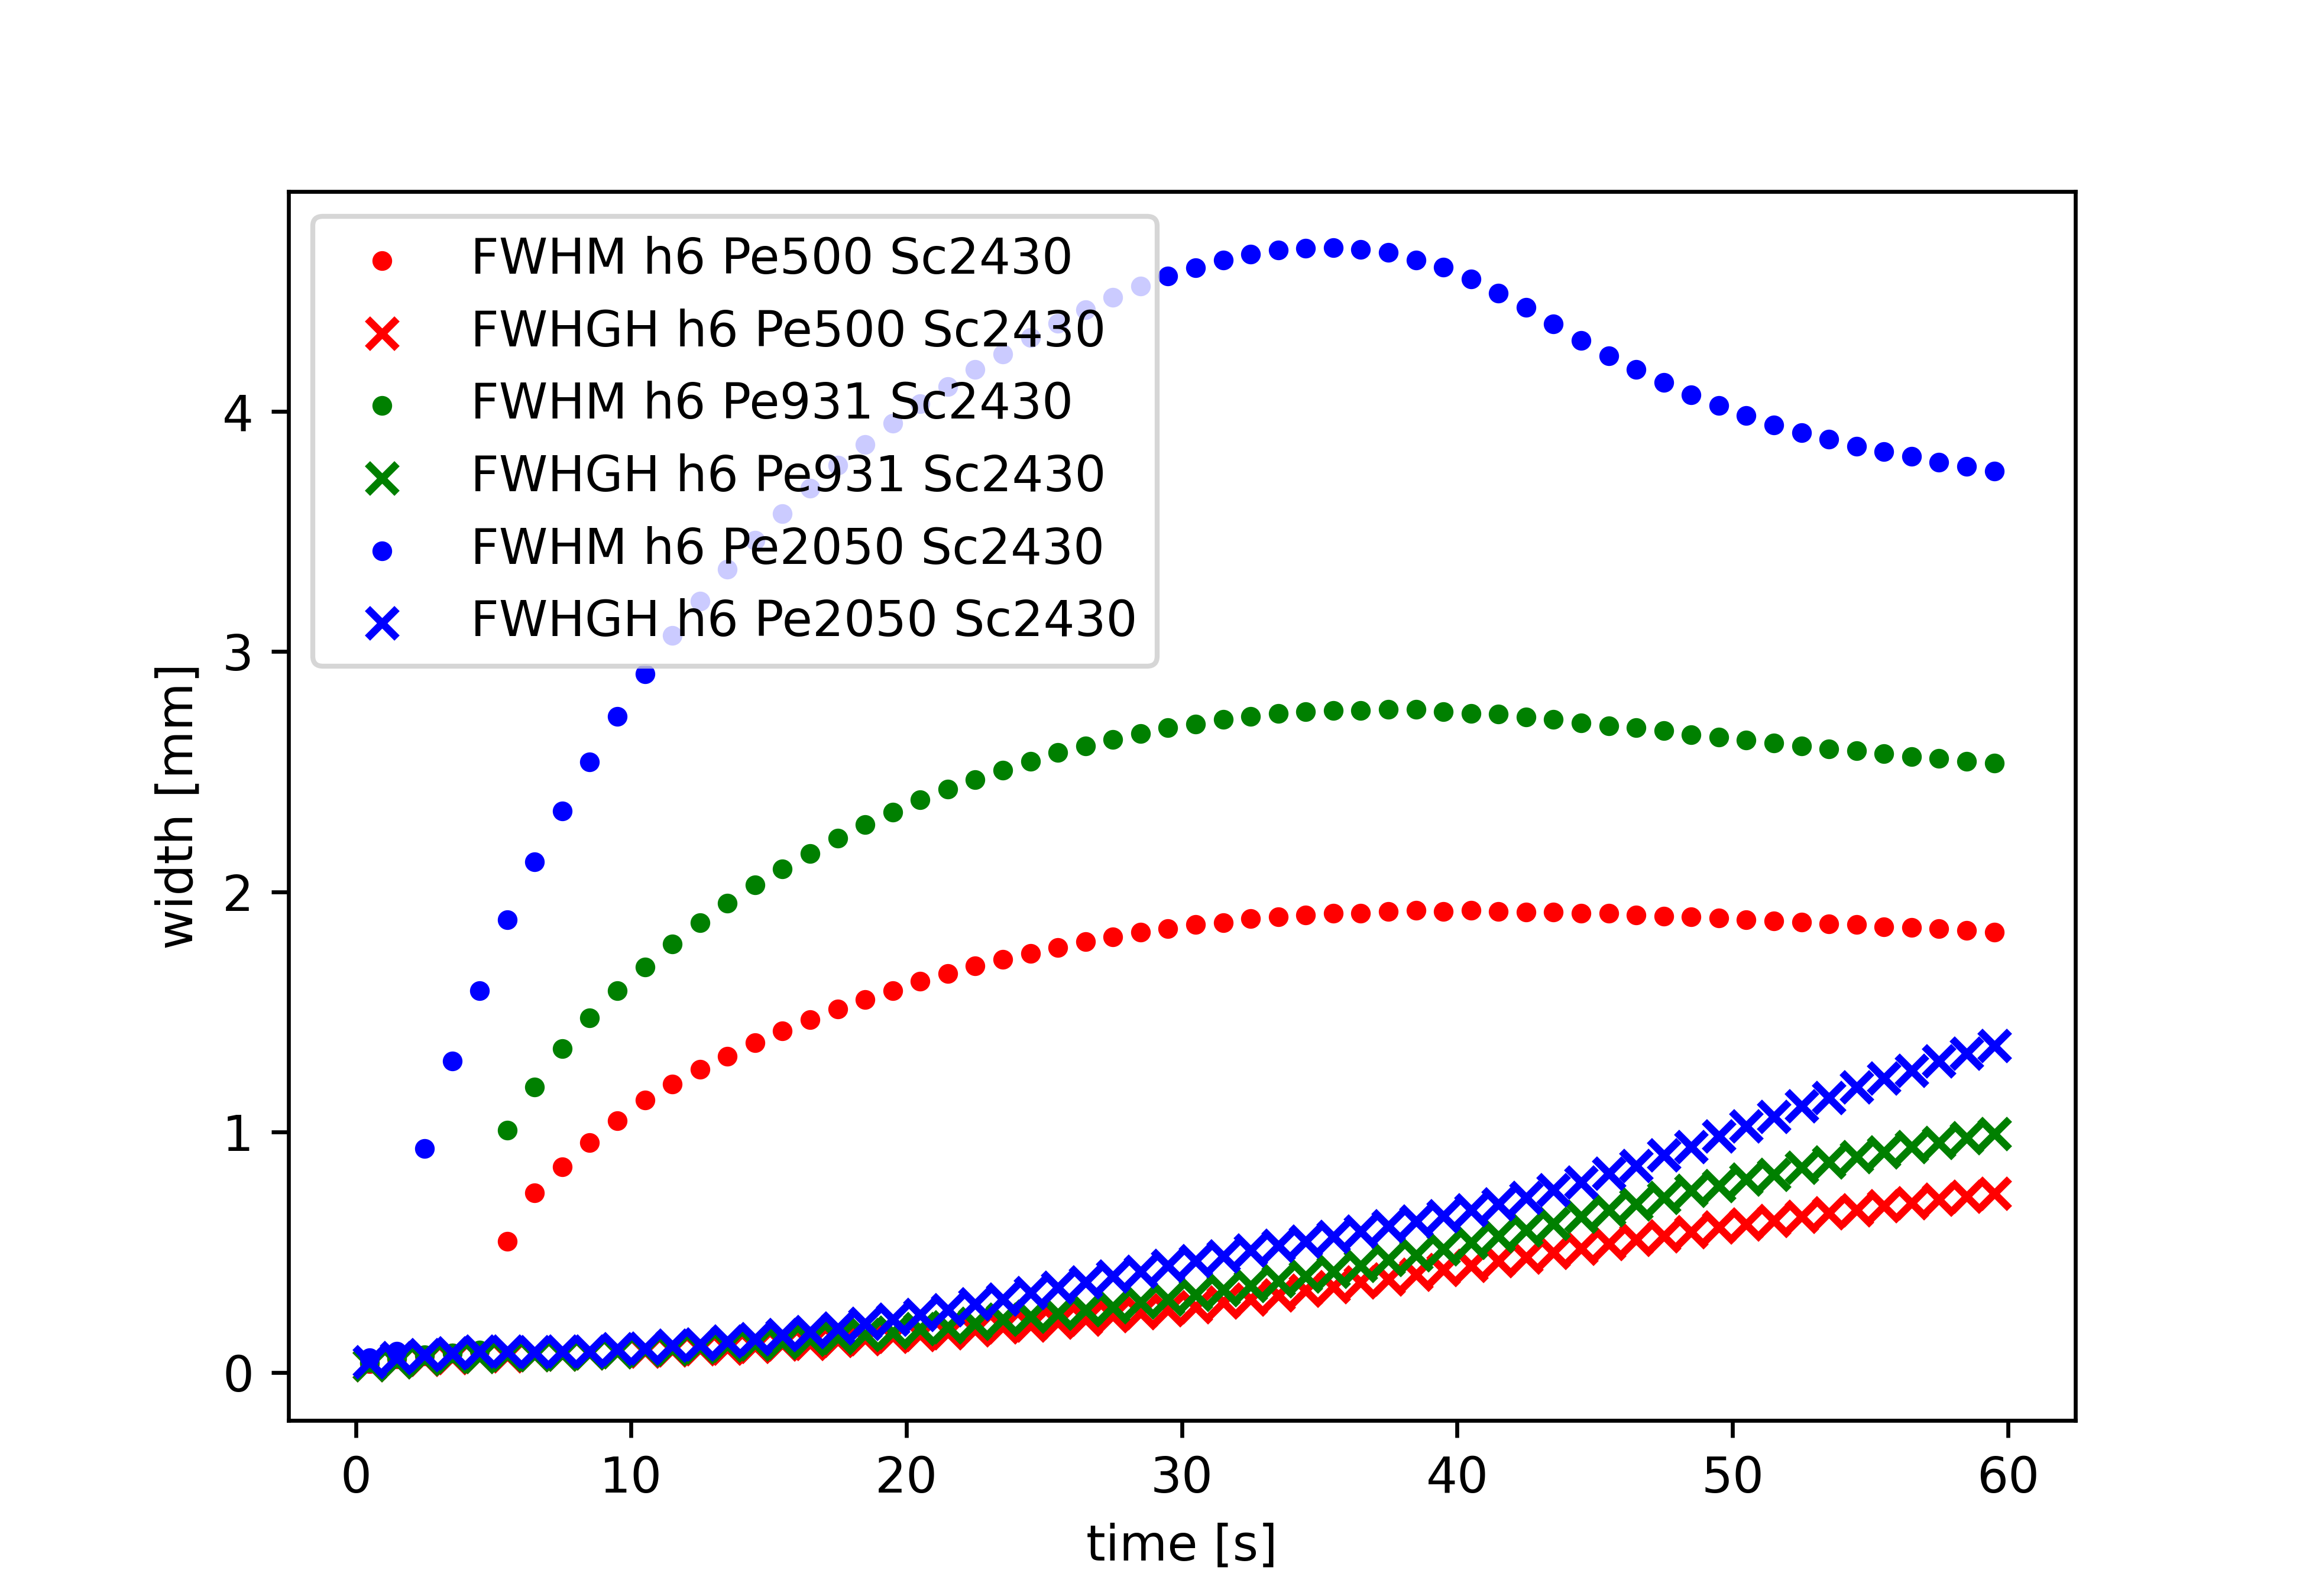
\includegraphics[width=.9\linewidth]{front_width_h6_Sc2430}
	\caption{front widths for h 0.6mm Sc 2430\label{fig: front_width_pos_h6_Sc2430}}
\end{figure}
A difference is that the width's growth seems to start delayed by about 10 to 18 seconds which is also visible within the 0.4mm case. Within \autoref{fig: plots_early} the concentration plots are shown for the gap height of 0.4mm and 0.6mm for a Peclet-Number of 931 and a Schmidt-Number of 12000 close to the inlet. Within these two plots it can seen that the initial spike in the front start decaying over time. The moment the value of $0.5 \cdot c_{c,max}$ falls into the region above 0 and the value at the back of the front the fronts width suddenly jumps to a higher value.
\begin{figure}[htb]
	\centering
	\subfloat[\centering h0.6mm case]{{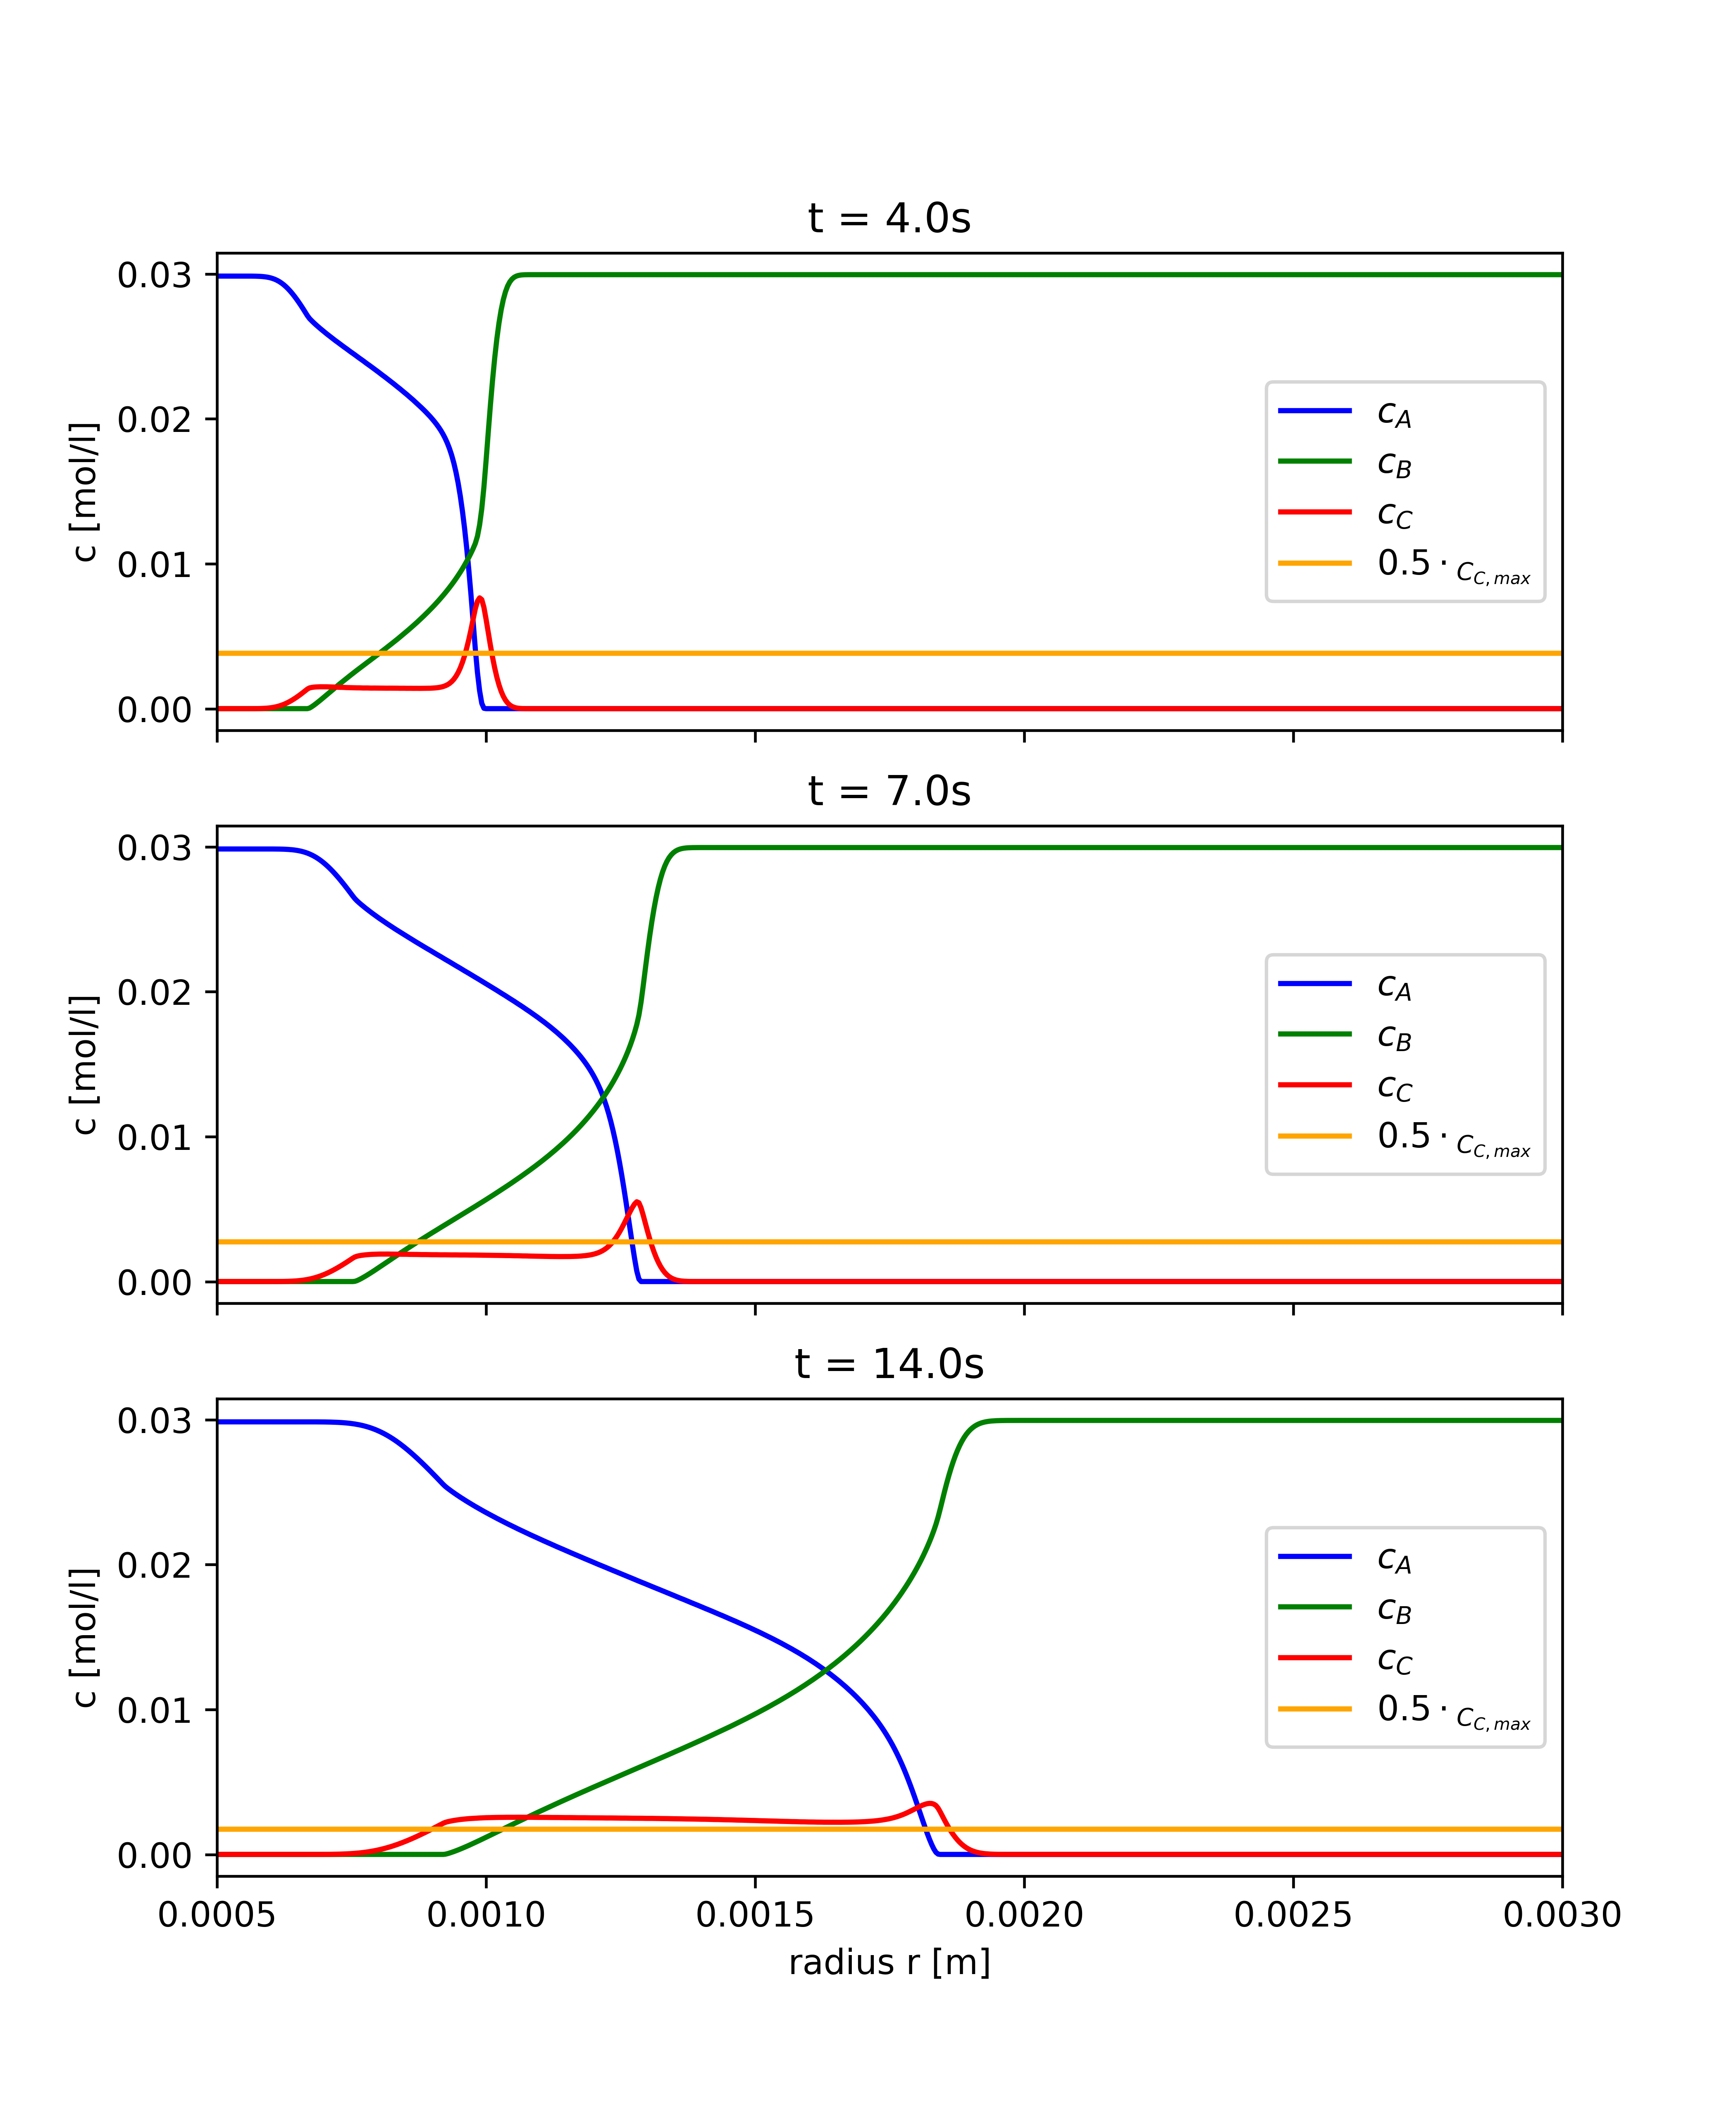
\includegraphics[angle=0, scale=0.41]{plot_h6r3_P931E2_S120E4_concentration-fluid_a_concentration-fluid_b_concentration-fluid_c} }}%
	\qquad
	\subfloat[\centering h0.4mm case]{{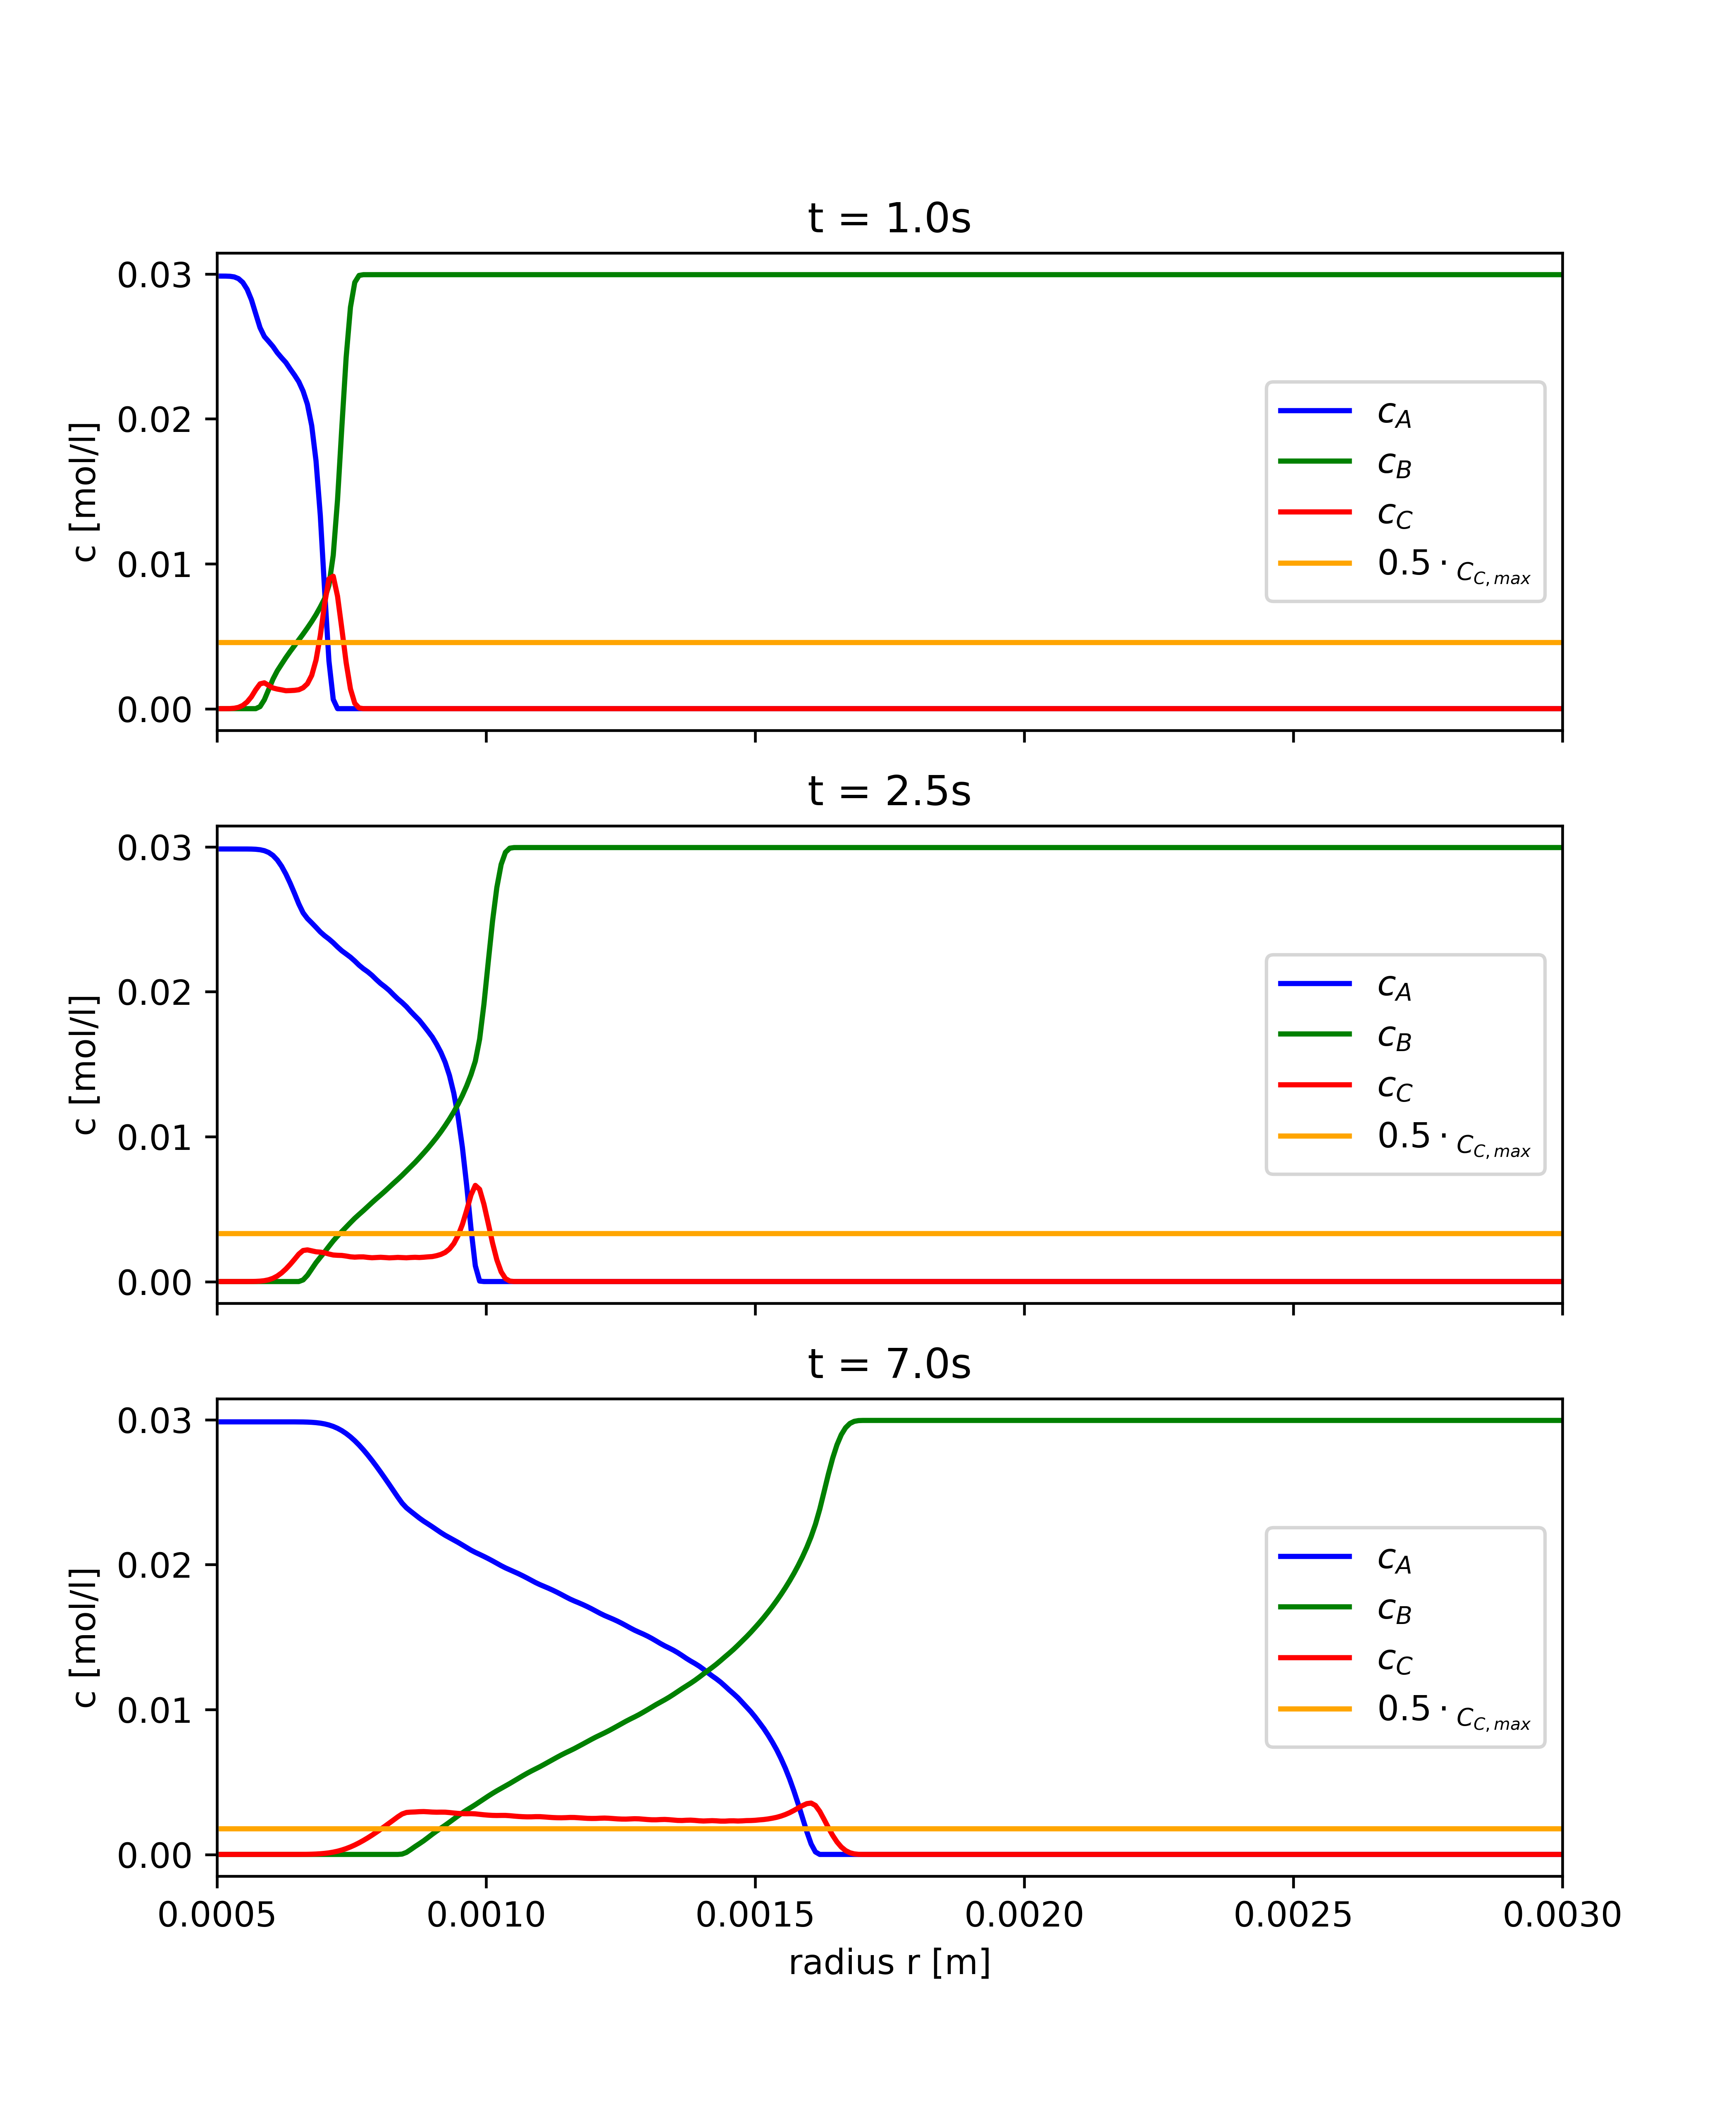
\includegraphics[angle=0, scale=0.41]{plot_h4r3_P931E2_S120E4_concentration-fluid_a_concentration-fluid_b_concentration-fluid_c copy} }}%
	\caption{concentration plots for Pe931 Sc12000}%
	\label{fig: plots_early}%
\end{figure}
The width at the middle of the reactor only reaches very low values and doesn't grow much within the 60 seconds runtime of the simulation. When looking at the behaviour of the middle width at the lower Schmid-Number the growth seems to start at around 20 seconds and the growth accelerates slowly until the end. The middle width reaches it's peak at times around 30 to 40 seconds for that Schmidt-Number. The growth is delayed for the FWHM width as well but not by the amount to be seen within the plot for $Sc = 12000$. The reason is the same one as explained with \autoref{fig: plots_early}.

All in all the front widths show different behaviour dependent on the conditions set for the cases. Changing the Schmidt-Number poses a significant change within the results as showed and discussed. The Peclet-Number seems to mostly influence the width's maximum peak value but doesn't change the general behaviour of the front.

\section{formed product}

Within this section the total product formed is investigated.

\begin{figure}[htbp]
	\centering
	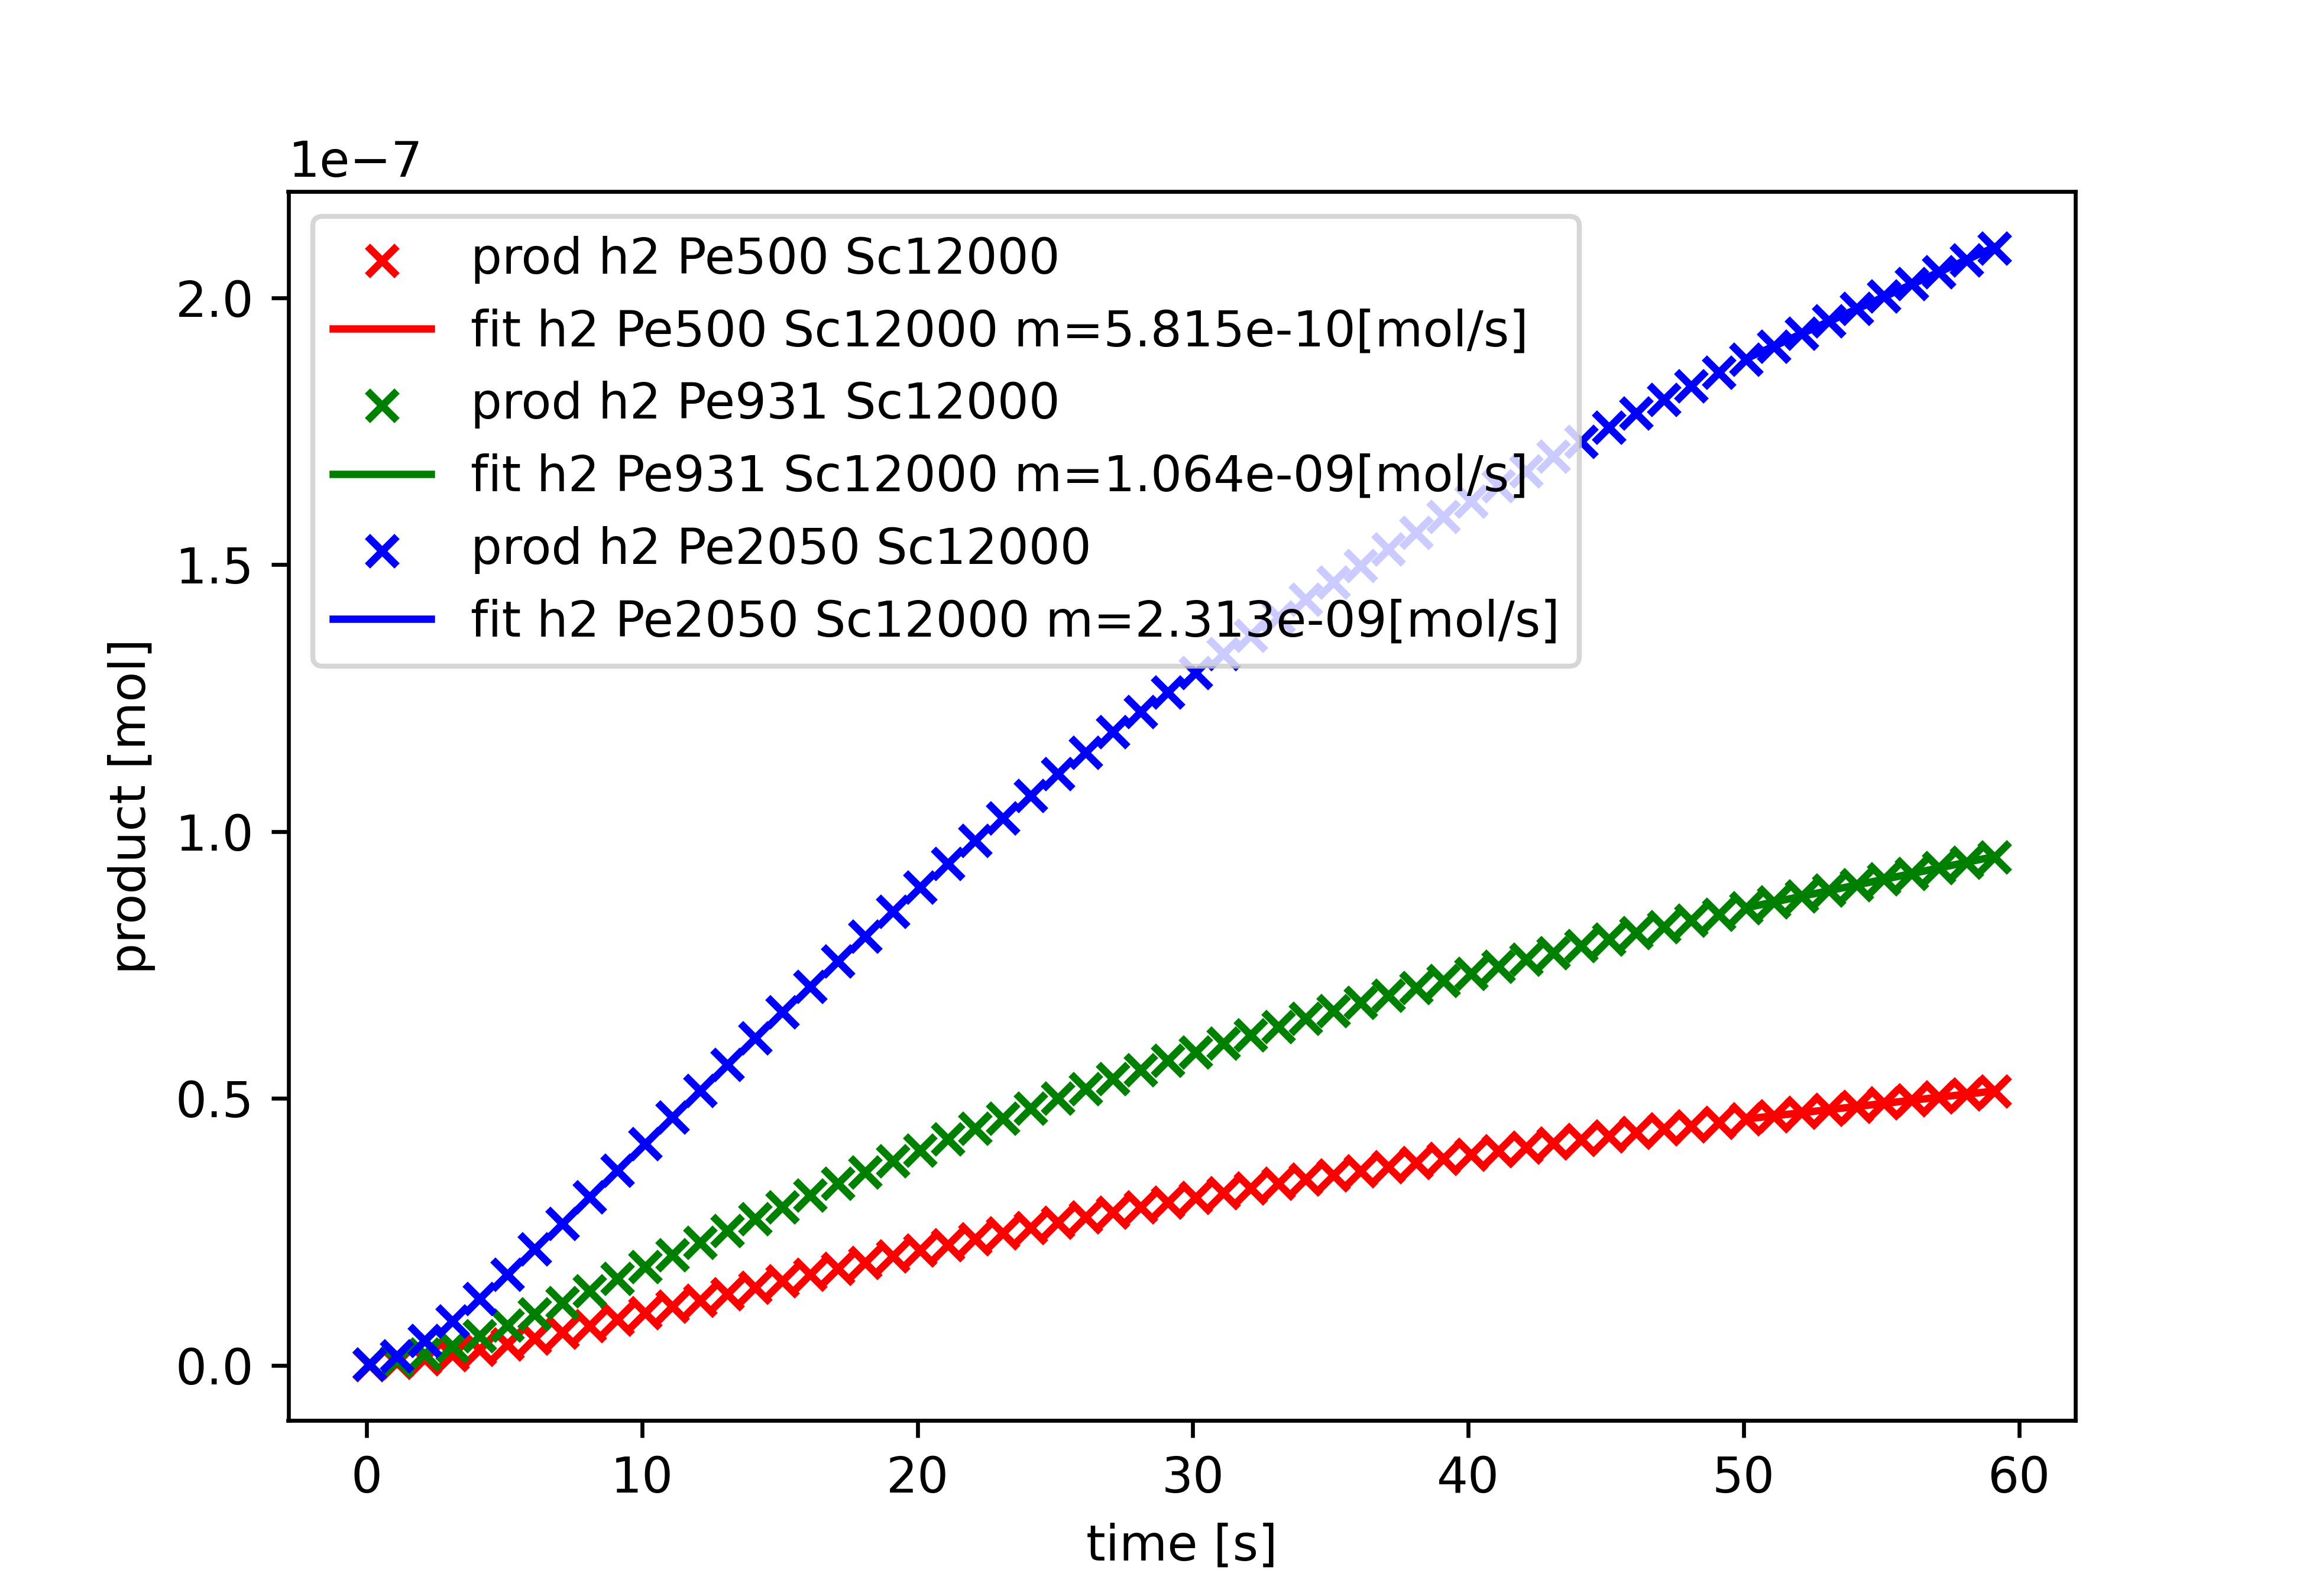
\includegraphics[width=.9\linewidth]{total_product_h2_Sc12000}
	\caption{total product for h 0.2mm Sc 12000\label{fig: total_prod_h2_Sc12000}}\bigskip
	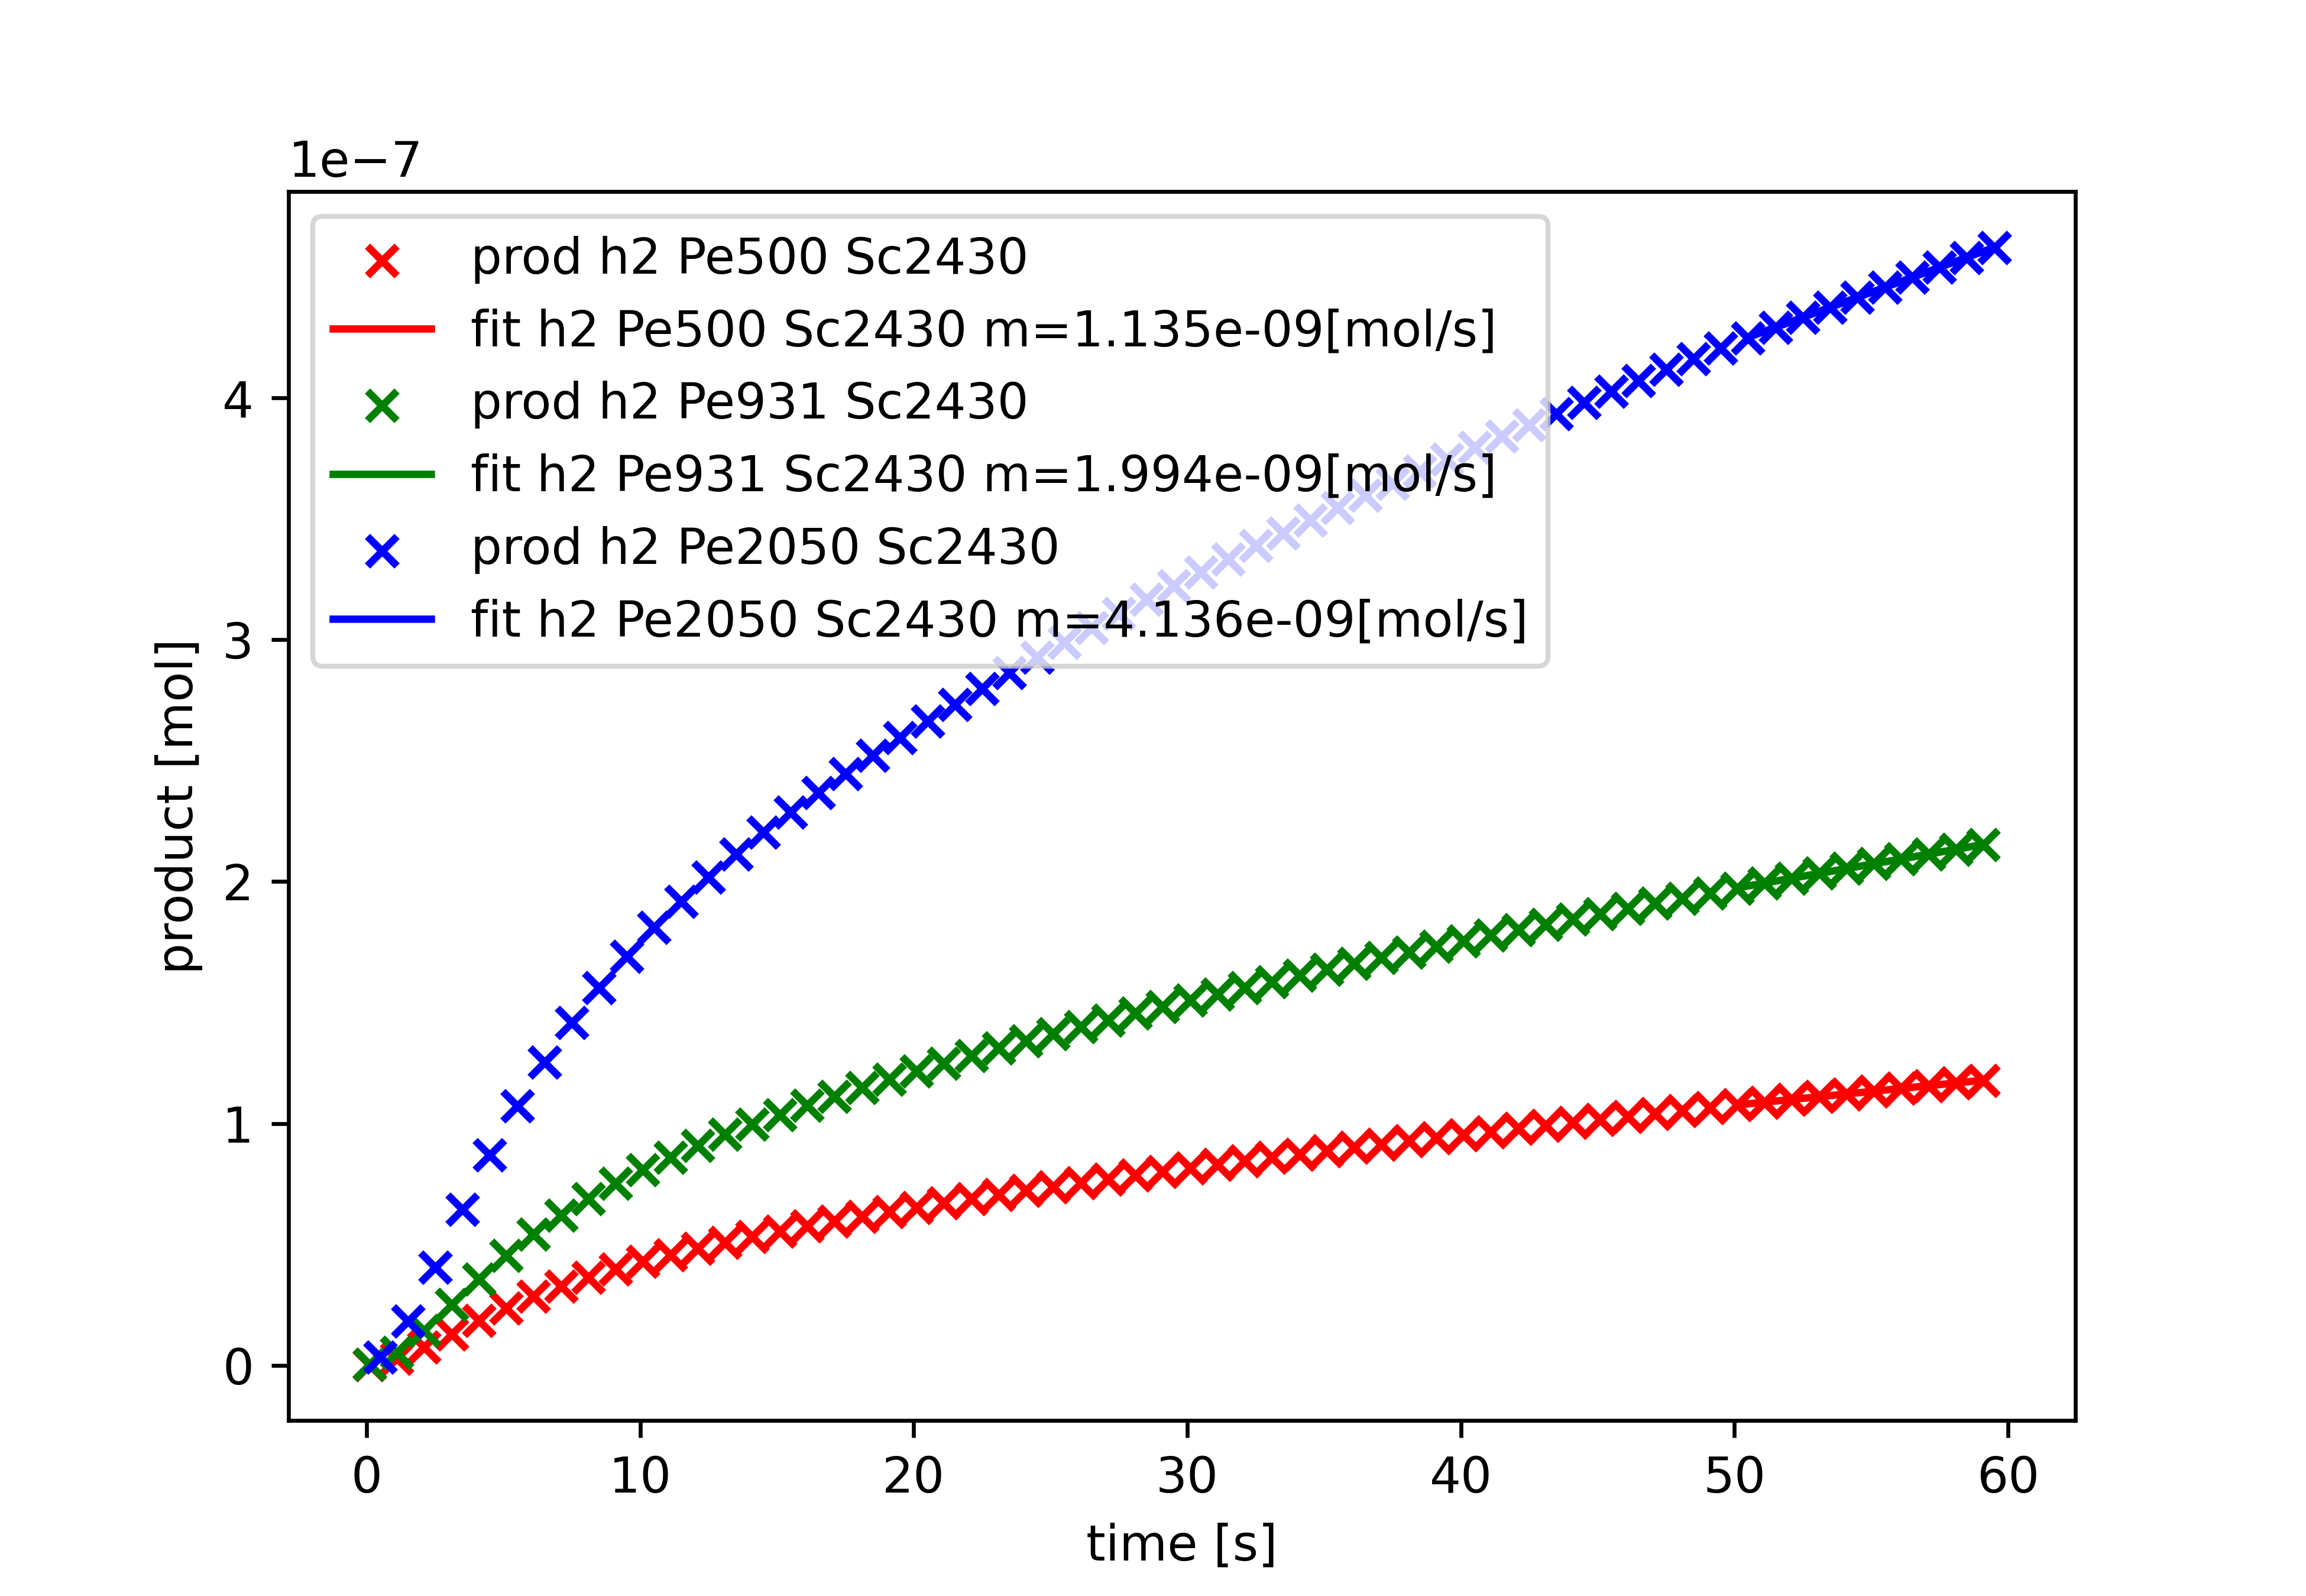
\includegraphics[width=.9\linewidth]{total_product_h2_Sc2430}
	\caption{total product for h 0.2mm Sc 2430\label{fig: total_prod_h2_Sc2430}}
\end{figure}

For the case with a gap height of 0.2mm the total product formed starts with a linear growth and then follows a square root like approach for all cases with a Schmidt-Number of 12000. Concluding out of this behaviour the production rate starts with a constant value and then decays over time. This is clearly visible for the case with a Peclet-Number of 2050 within the $Sc = 2430$ plot. The difference when lowering the Schmidt-Number is that the initial constant growth rate increases and the decay starts earlier.
\begin{figure}[htb]
	\centering
	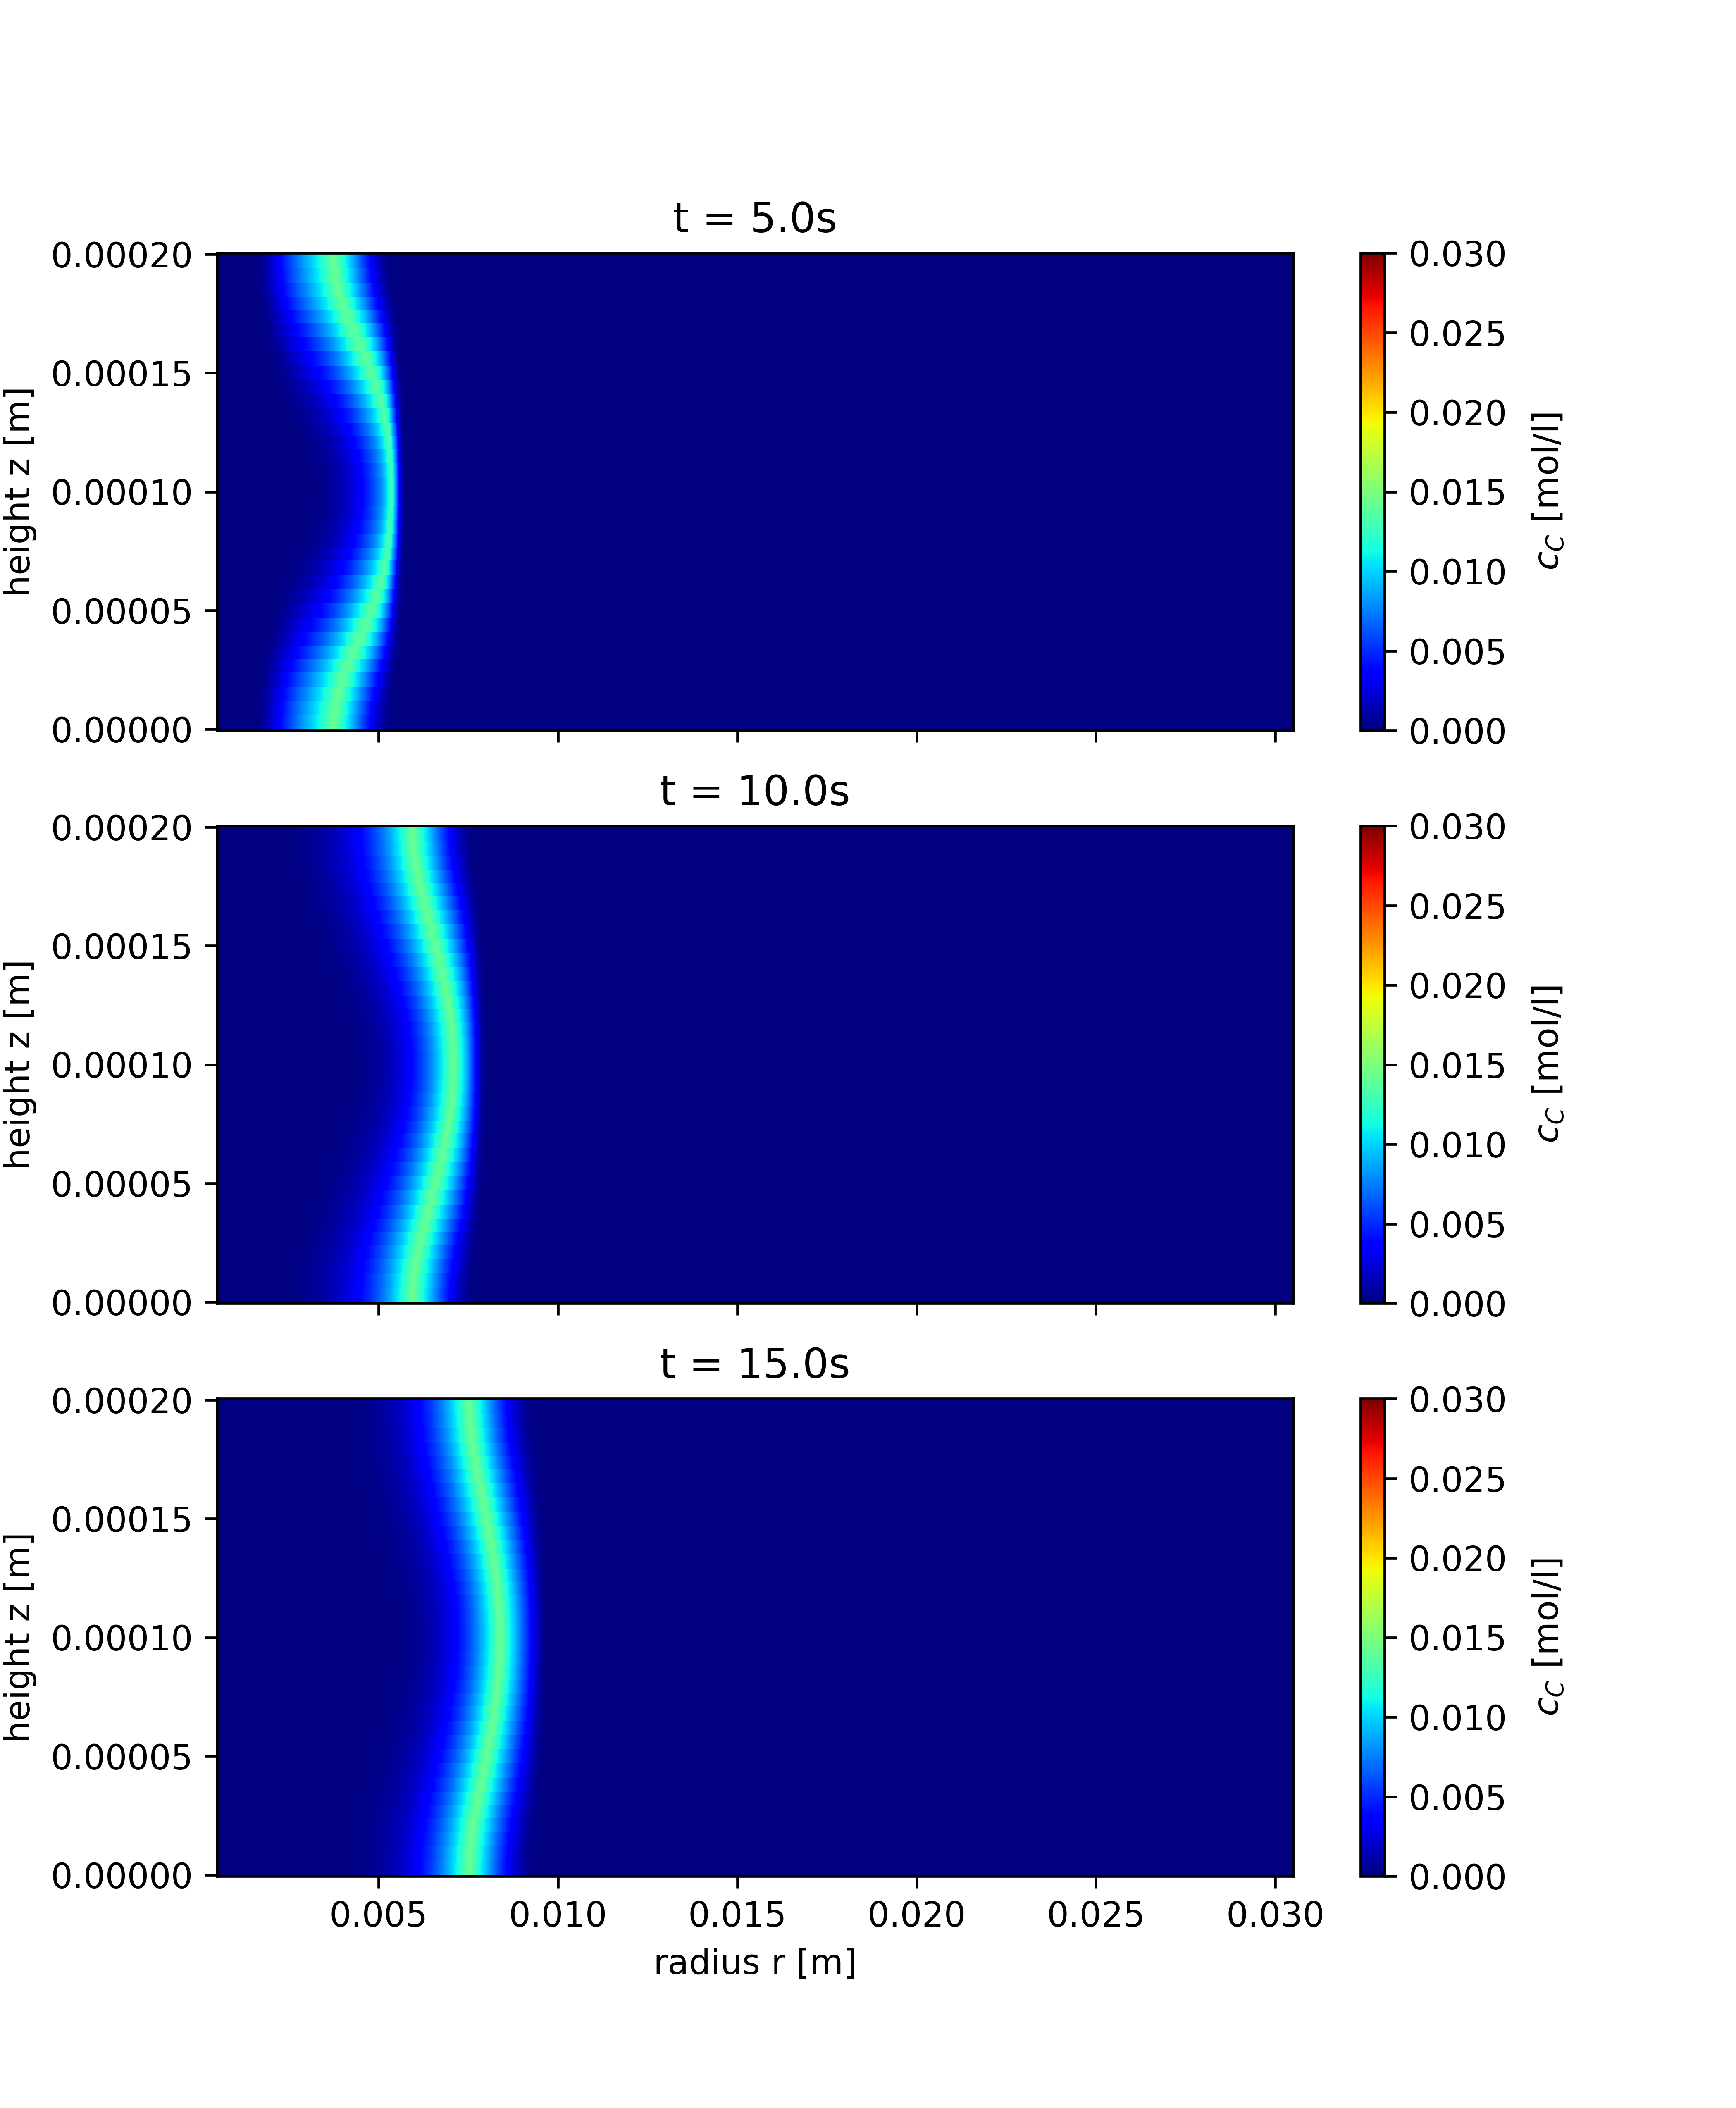
\includegraphics[width=0.7\textwidth]{field_h2r3_P205E3_S243E3_concentration-fluid_c}
	\caption{front shape for Pe2050 Sc2430}
	\label{fig: front_h2_late}
\end{figure}
In \autoref{fig: front_h2_late} the product concentration fields are shown for a time of 5 seconds which is within the phase of constant production rate, a time of 10 seconds which marks the point of production rate decay and a time of 15 seconds which is in the decaying phase. From these fronts it can be seen that the production rate is constant until the front starts to experience a more and more growing influence of diffusion. This can be seen by looking at the width and overall product concentration in the front of the front. At 5 seconds the width at half the gap height is small and nearly no product is visible in the space in front of the front. At 10 seconds that does change. The middle width has gained the same shape is the widths above and below it and a slight amount of product starts appearing at coordinates with higher radial values. This effect is even more visible at 15 seconds. Apparently the described effect is not clearly visible within the widths plot of this case as shown in \autoref{fig: front_width_pos_h2_Sc2430} due to the way the middle with is calculated. Within the widths plot it is visible that the middle width stops growing at the time of 10 seconds when the diffusive influence starts raising. 

\begin{figure}[htbp]
	\centering
	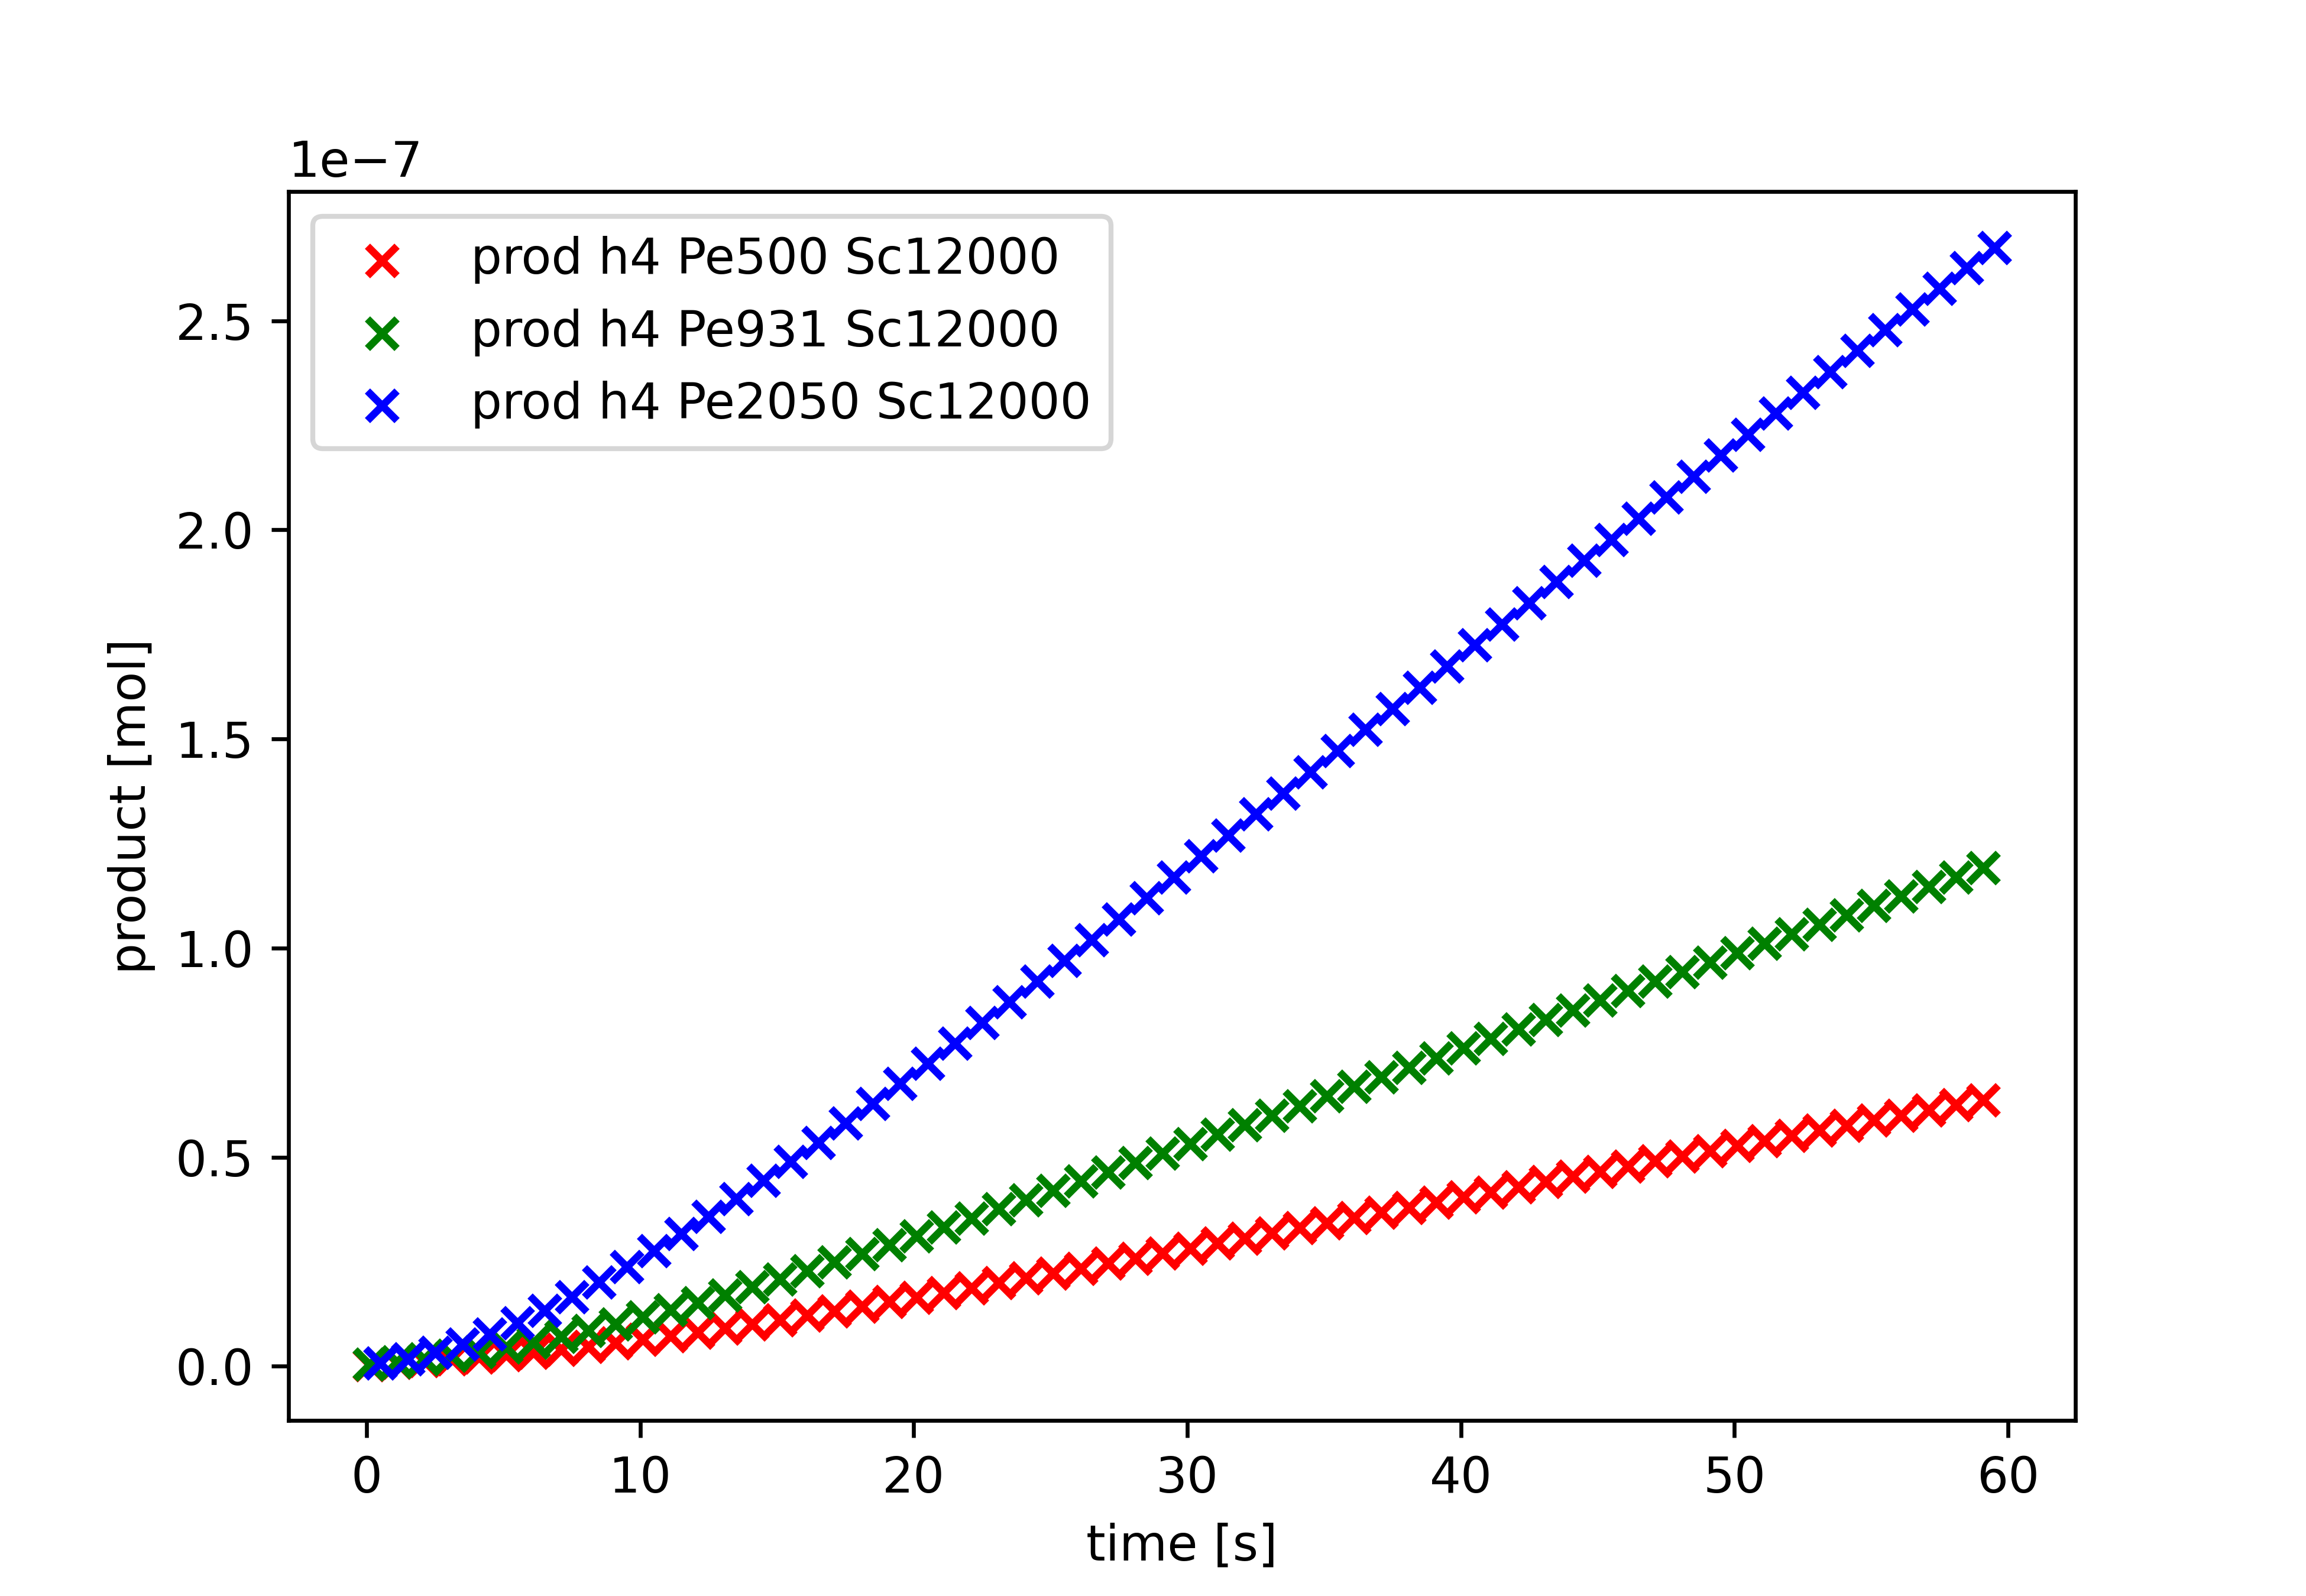
\includegraphics[width=.9\linewidth]{total_product_h4_Sc12000}
	\caption{total product for h 0.4mm Sc 12000\label{fig: total_prod_h4_Sc12000}}\bigskip
	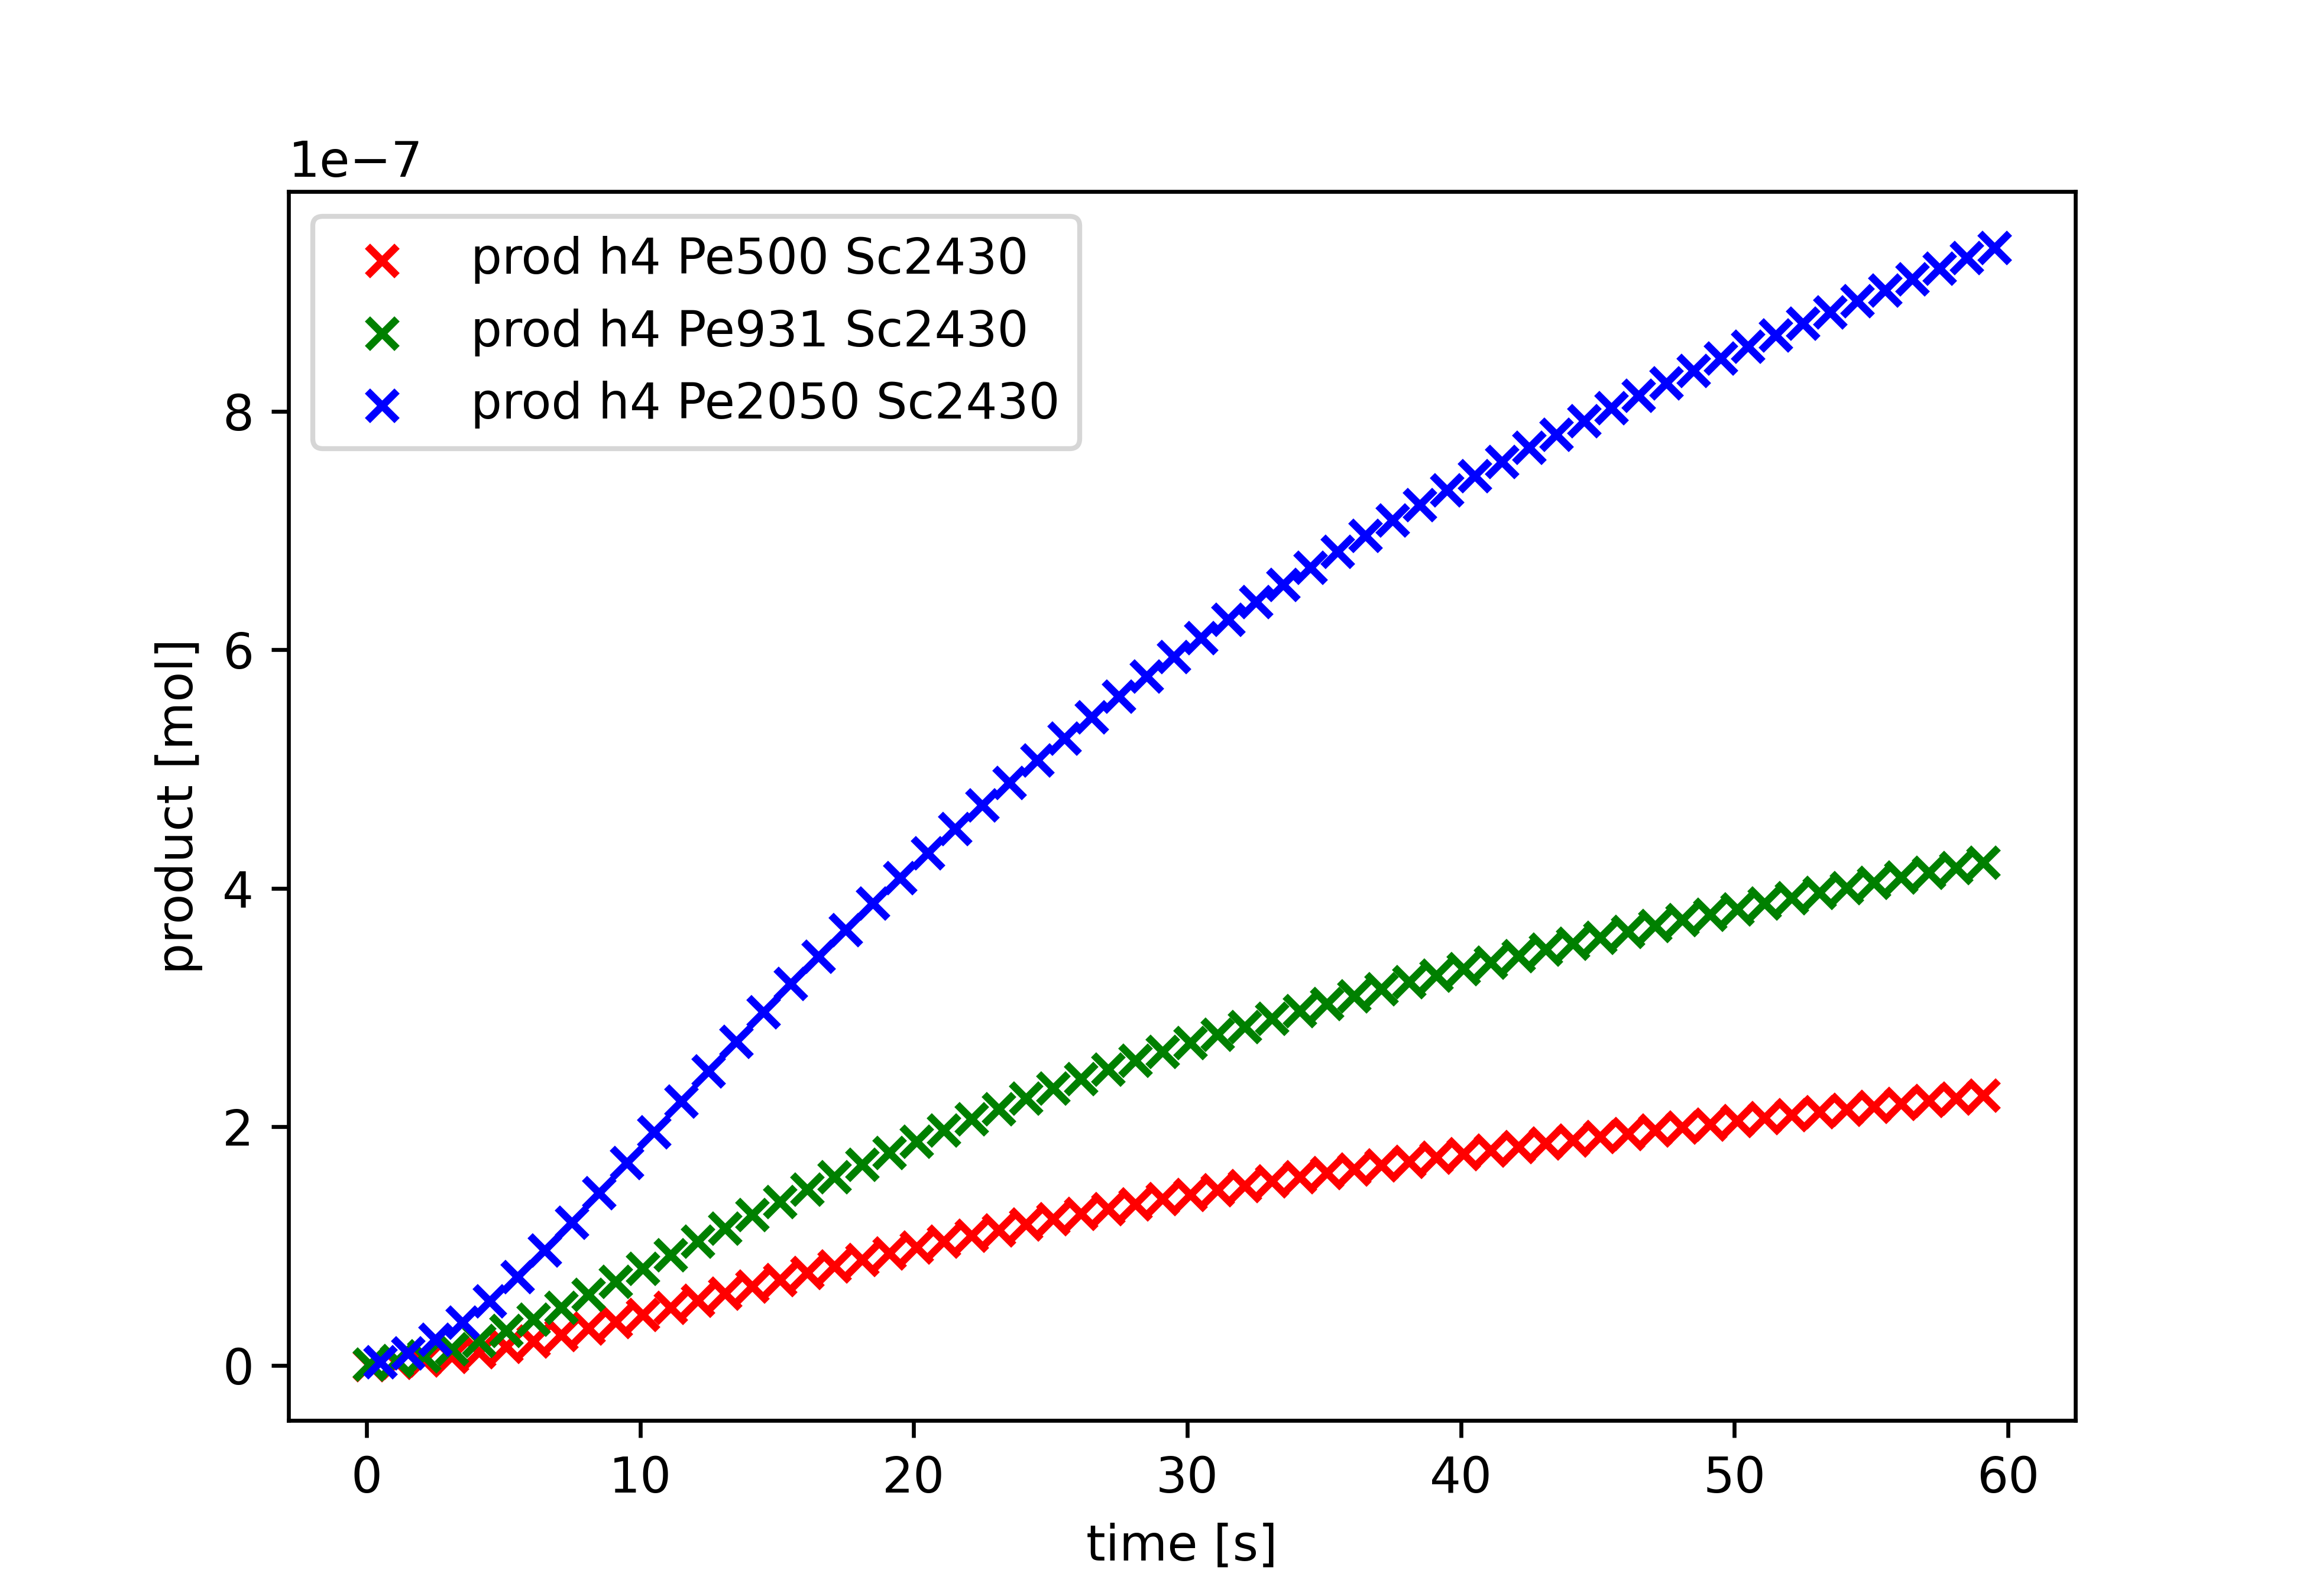
\includegraphics[width=.9\linewidth]{total_product_h4_Sc2430}
	\caption{total product for h 0.4mm Sc 2430\label{fig: total_prod_h4_Sc2430}}
\end{figure}

\begin{figure}[htbp]
	\centering
	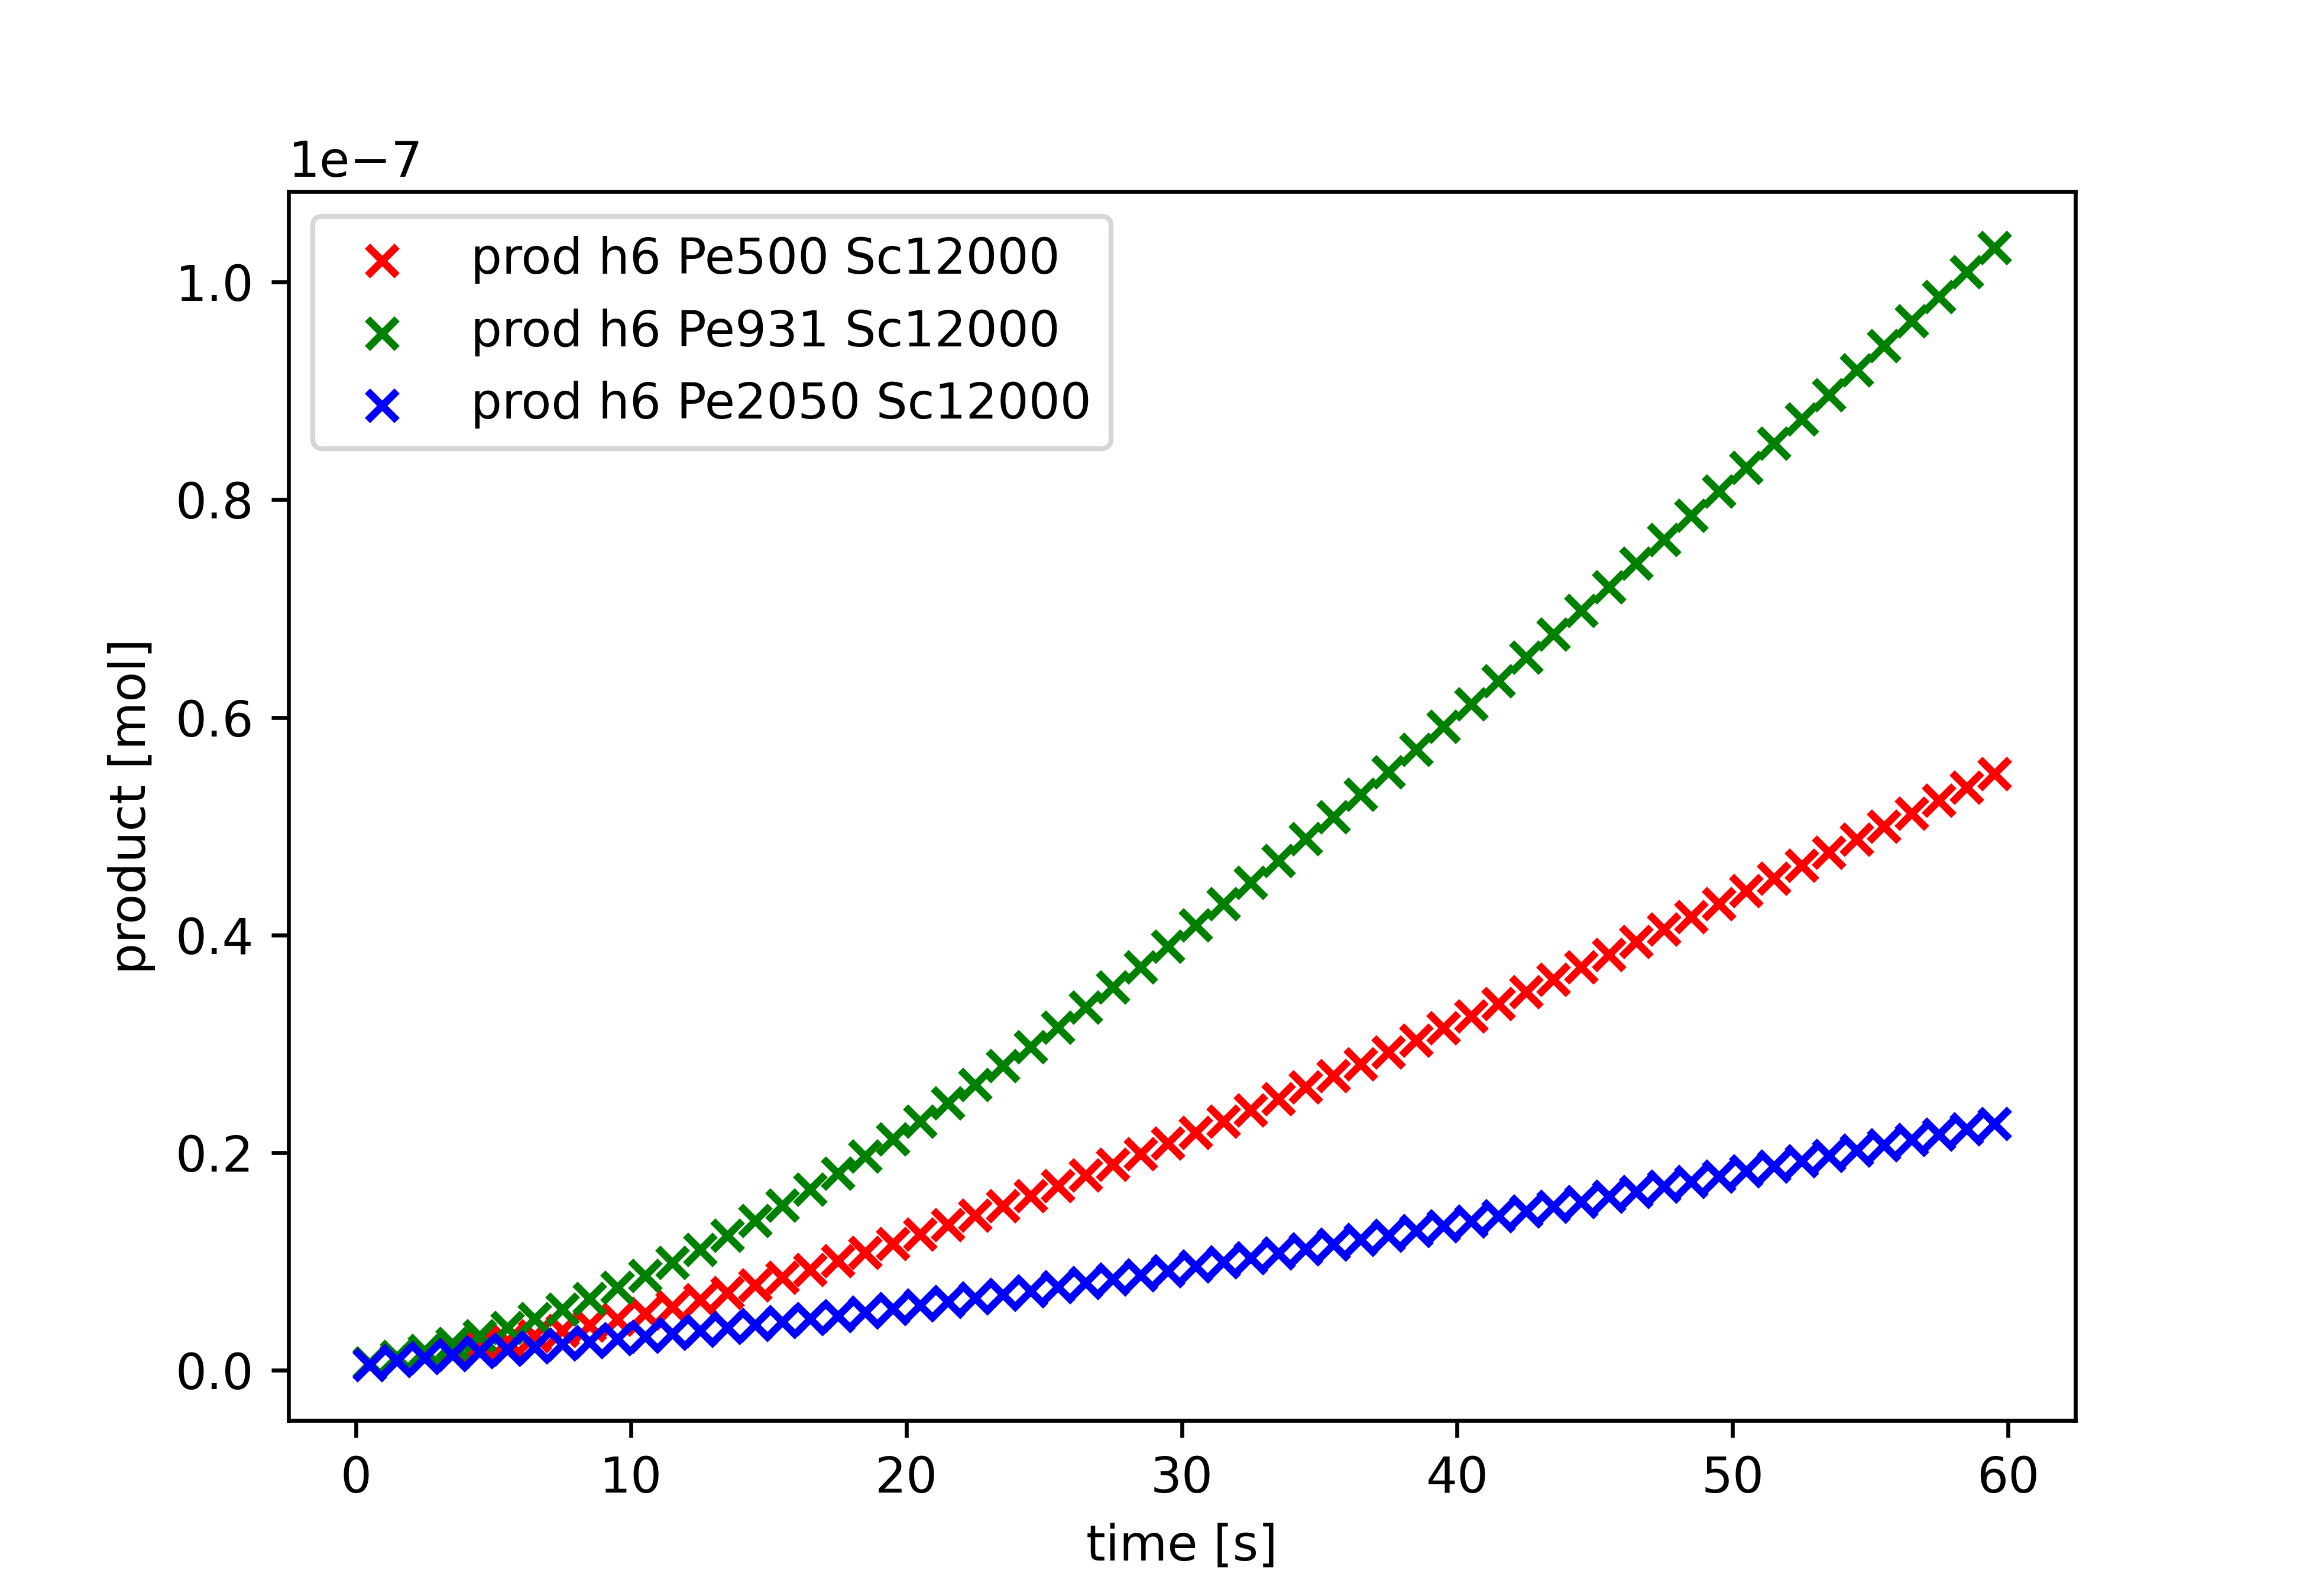
\includegraphics[width=.9\linewidth]{total_product_h6_Sc12000}
	\caption{total product for h 0.6mm Sc 12000\label{fig: total_prod_h6_Sc12000}}\bigskip
	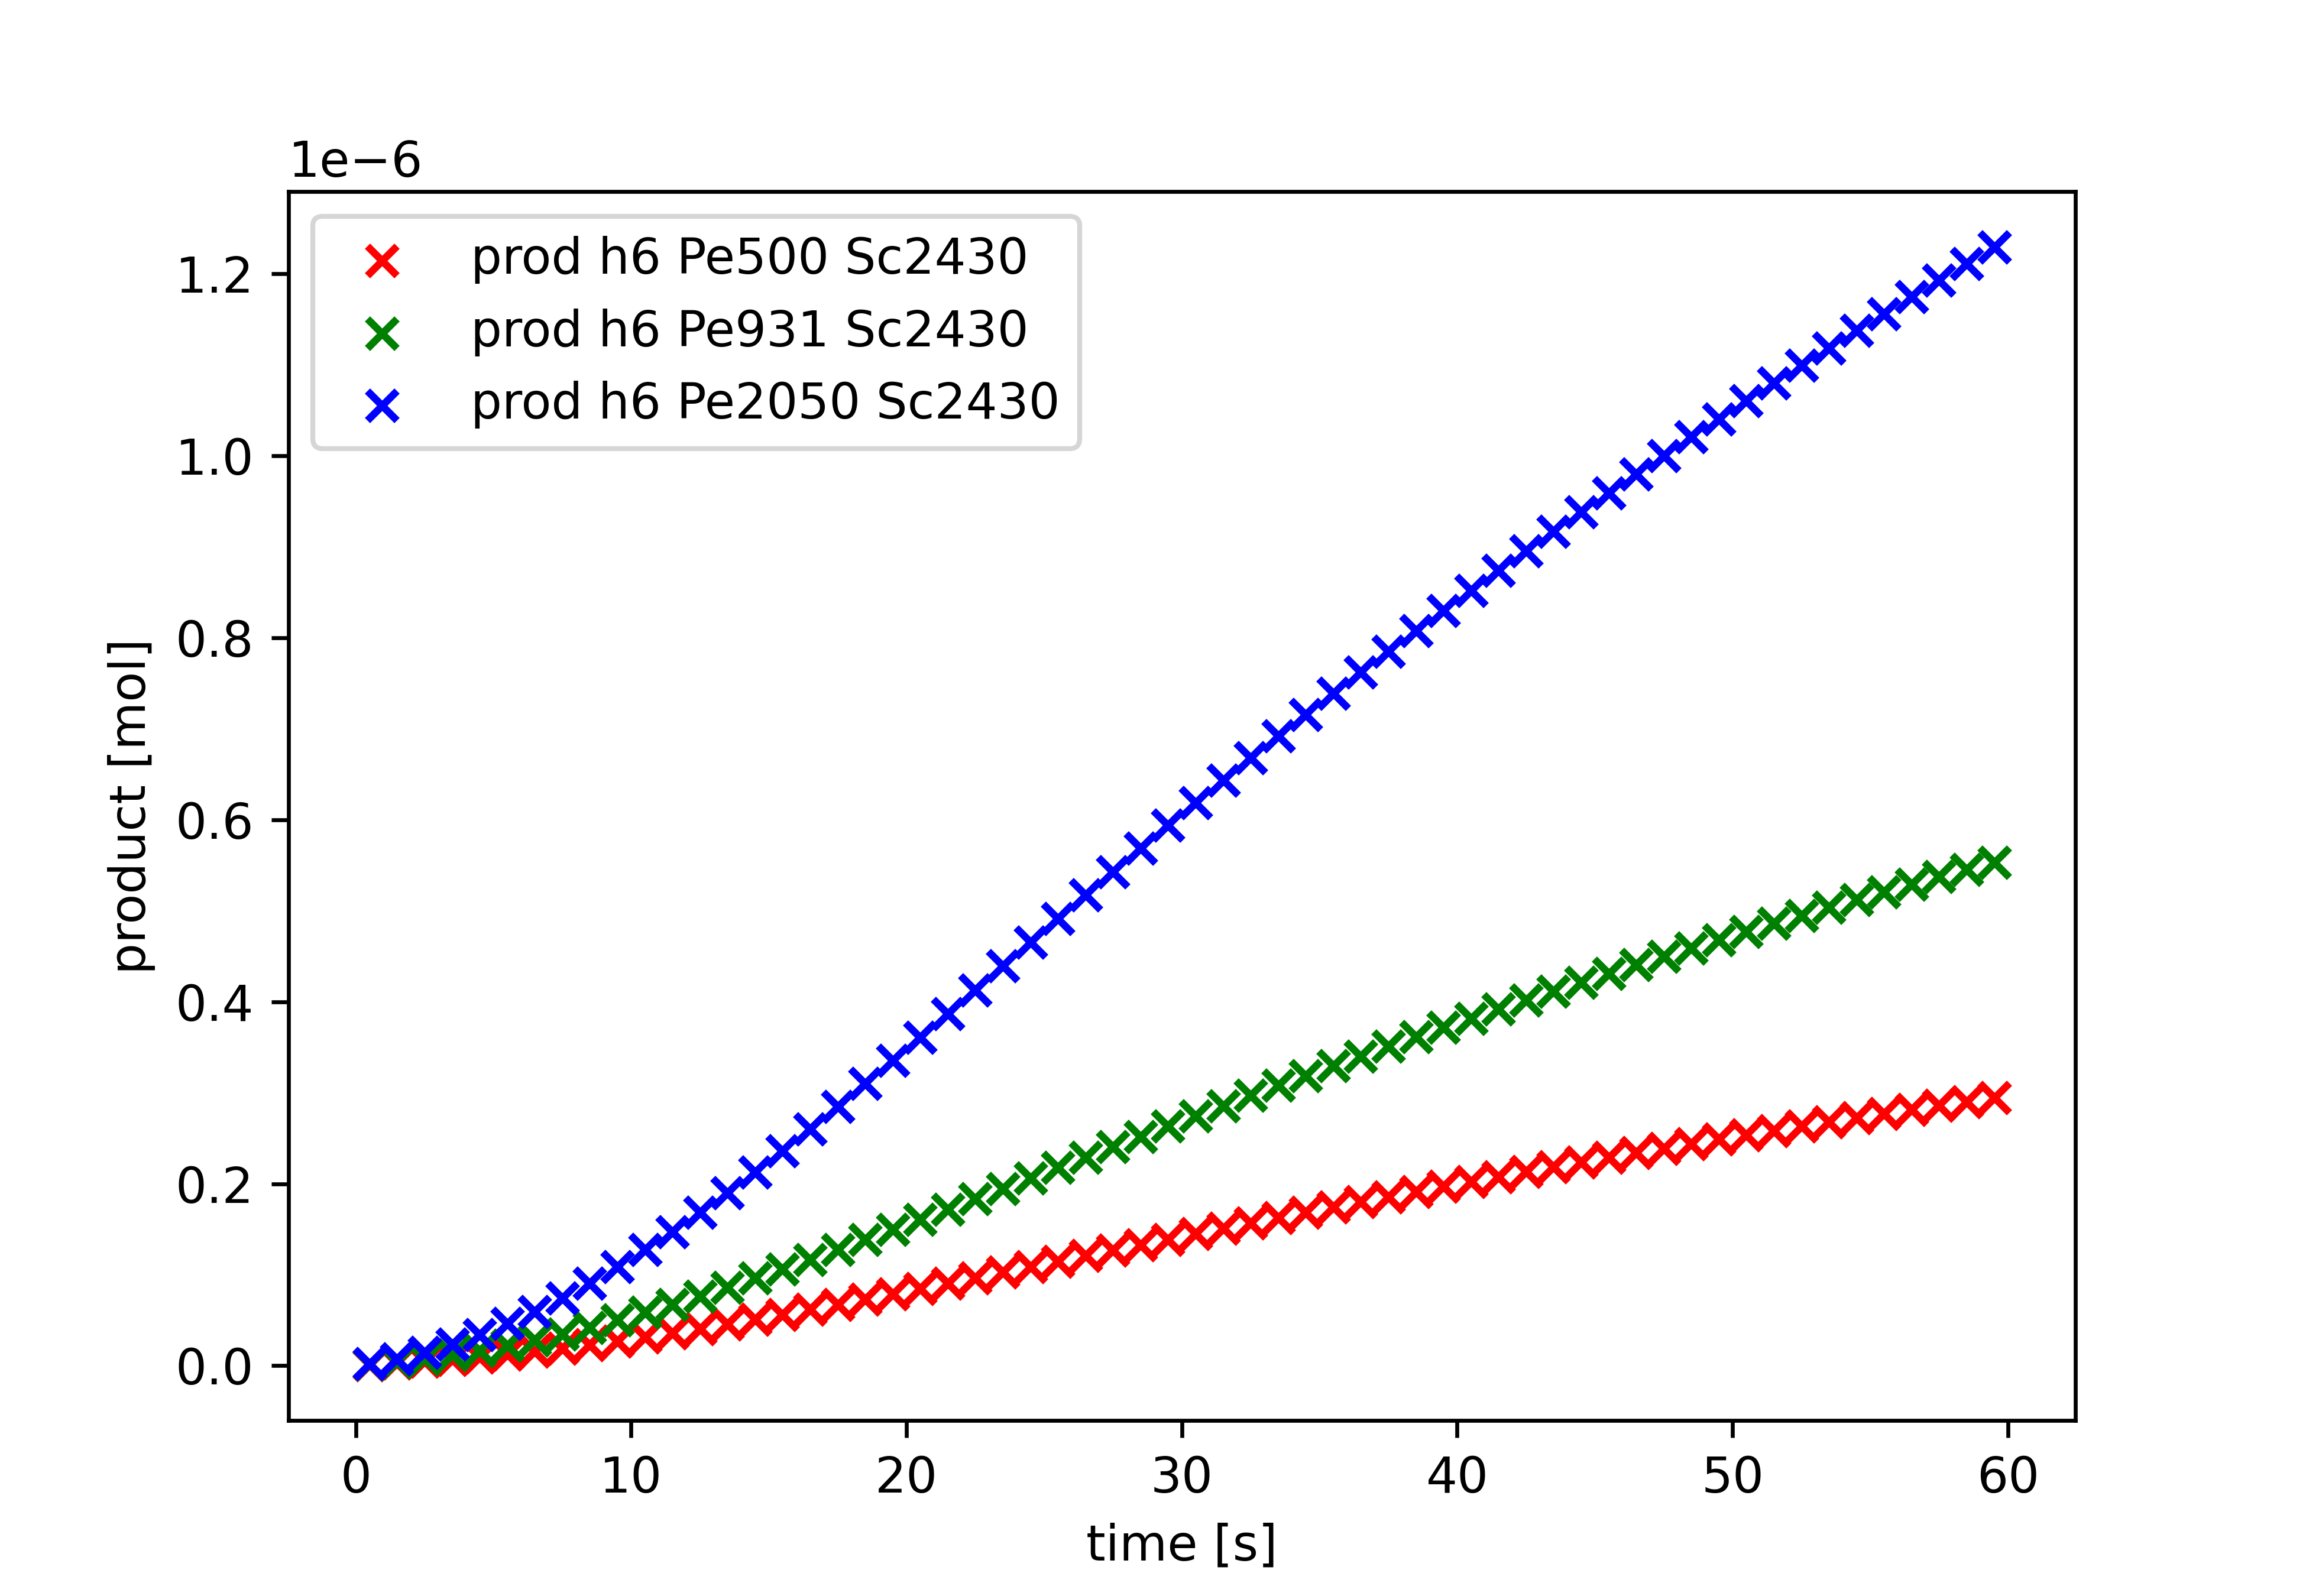
\includegraphics[width=.9\linewidth]{total_product_h6_Sc2430}
	\caption{total product for h 0.6mm Sc 2430\label{fig: total_prod_h6_Sc2430}}
\end{figure}

\end{document}